\PassOptionsToClass{}{beamer}
\documentclass[serif, aspectratio=169]{beamer}
\usepackage[utf8]{inputenc}
\usepackage{amsmath,esint}
\usepackage[british]{babel}
\usetheme{Warsaw}
\usecolortheme{rose}
\usepackage{comment}
\usepackage{pgfplots}
\usepackage{ mathrsfs }
\usepackage{gensymb}
\usepackage{color}
\usepackage{tkz-euclide}
\usetkzobj{all}
\usepackage{tkz-fct}  
\usetikzlibrary{calc}
\usepackage[ruled]{algorithm2e}
\usepackage{tikz}
\usepackage{animate}
\usepackage{ragged2e}
\usepackage{mwe}

\usepackage{tabstackengine}
\setstackEOL{\cr}

\DeclareMathOperator*{\minimize}{minimize}

\addtobeamertemplate{navigation symbols}{}{%
    \usebeamerfont{footline}%
    \usebeamercolor[fg]{footline}%
    \hspace{1em}%
    \insertframenumber/\inserttotalframenumber
}

\makeatletter
\newcommand\titlegraphicii[1]{\def\inserttitlegraphicii{#1}}
\titlegraphicii{}
\setbeamertemplate{title page}
{
  \vspace{0.3in}
  \vbox{}

  \begin{centering}
    \begin{beamercolorbox}[sep=8pt,center]{title}
      \usebeamerfont{title}\inserttitle\par%
      \ifx\insertsubtitle\@empty%
      \else%
        \vskip0.25em%
        {\usebeamerfont{subtitle}\usebeamercolor[fg]{subtitle}\insertsubtitle\par}%
      \fi%     
    \end{beamercolorbox}%
    \vskip1em\par
    \begin{beamercolorbox}[sep=8pt,center]{date}
      \usebeamerfont{date}\insertdate
    \end{beamercolorbox}%\vskip0.5em
    \begin{beamercolorbox}[sep=8pt,center]{author}
      \usebeamerfont{author}\insertauthor
    \end{beamercolorbox}
    \begin{beamercolorbox}[sep=8pt,center]{institute}
      \usebeamerfont{institute}\insertinstitute
    \end{beamercolorbox}
  \end{centering}
  %\vfill
}
\makeatother

\author{Mitesh M. Khapra}
\title{CS7015 (Deep Learning) : Lecture 7}
\subtitle{Autoencoders and relation to PCA, Regularization in autoencoders, Denoising autoencoders, Sparse autoencoders, Contractive autoencoders}
\institute{Department of Computer Science and Engineering\\ Indian Institute of Technology Madras}
\date{}
\titlegraphic{
\includegraphics[height=1cm,width=2cm]{images/iitm_logo.png}}


\begin{document}


\def\alpha{8} 

\newcommand\myheading[1]{%
\par\bigskip
{\Large\bfseries#1}\par\smallskip}


\newcommand\derivative[5]{%
    \tkzDefPointByFct[draw](#1) \tkzGetPoint{start}
  \tkzDefPointByFct[draw](#2) \tkzGetPoint{end}
  \draw[thin,|-|,yshift=-3pt] (start) -- node[black,fill=white,#5] {#3}(start-|end);  
  \draw[thin,|-|,xshift=3pt] (start-|end) -- node[black,fill=white,right] {#4}(end); 
  %\draw[thin] (start) --(end); 
}
\maketitle
\begin{frame}
	\myheading{Module 7.1:  Introduction to Autoencoders }
\end{frame}


\begin{frame}
	\begin{columns}  
    		\column{0.5\textwidth}    
    		\begin{overlayarea}{\textwidth}{\textheight}        
        		\vspace{5pt}
			\tikzstyle{input_neuron}=[circle,draw=red!50,fill=red!10,thick,minimum size=6mm]
\tikzstyle{hidden_neuron}=[circle,draw=blue!50,fill=cyan!10,thick,minimum size=6mm]
\tikzstyle{output_neuron}=[circle,draw=green!50,fill=green!10,thick,minimum size=6mm]
\tikzstyle{input}=[circle,draw=black!50,fill=black!20,thick,minimum size=6mm]

\begin{center}
\begin{tikzpicture}

\node [input_neuron] (neuron01) at (6.5,4.5) {};
\node [input_neuron] (neuron02) at (7.5,4.5){};
\node [input_neuron] (neuron03) at (8.5,4.5) {};
\node [input_neuron] (neuron04) at (9.5,4.5) {};
\node [input_neuron] (neuron05) at (10.5,4.5) {};
\node [hidden_neuron] (neuron51) at (7,6) {} ;
\node [hidden_neuron] (neuron52) at (8,6)  {};
\node [hidden_neuron] (neuron53) at (9,6)  {};
\node [hidden_neuron] (neuron54) at (10,6)  {};

\node [output_neuron] (neuron11) at (6.5,7.5)  {};
\node [output_neuron] (neuron12) at (7.5,7.5)  {};
\node [output_neuron] (neuron13) at (8.5,7.5)  {};
\node [output_neuron] (neuron14) at (9.5,7.5)  {};
\node [output_neuron] (neuron15) at (10.5,7.5)  {};

\node[text width=0.01cm] at (11.2,4.5) {$\mathbf{x_i}$};
\node[text width=0.007cm] at (7.7,5.25) {$W$};
\node[text width=0.01cm] at (10.7,6) {$\mathbf{h}$};
\node[text width=0.007cm] at (7.7,6.75) {$W^*$};
\node[text width=0.01cm] at (11.2,7.5) {$\mathbf{\hat{x}_i}$};

\draw[red!100,thick,solid,rounded corners=15pt] (6,4) rectangle (11,5);
\draw[red!100,thick,solid,rounded corners=15pt] (6.5,5.5) rectangle (10.5,6.5);
\draw[red!100,thick,solid,rounded corners=15pt] (6,7) rectangle (11,8);

\draw[thick,->] (8.5,5) -- (8.5,5.5);

\draw[thick,->] (8.5,6.5) -- (8.5,7);


\end{tikzpicture}
\end{center}
                
        		\vspace{-24pt}

			\begin{align*}
				\onslide<4->{\mathbf{h} &= g(W\mathbf{x_i} + \mathbf{b})}\\
				\onslide<6->{\mathbf{\hat{x}_i} &= f(W^*\mathbf{h} + \mathbf{c} )}
			\end{align*}

			\if 0
				\only<4->
					{
	            			\begin{align*}
    		        				\mathbf{h} = g(W\mathbf{x_i} +\mathbf{b})
	        		    	\end{align*}
    	    		}
    		    	\vspace{-0.5cm}
        			\only<6->
        			{
	            		\begin{align*}
						    \hspace{1.25cm}
	        			    \mathbf{\hat{x}_i} = f(W^*\mathbf{h} +\mathbf{c})
            			\end{align*}            
	        		}
			\fi 

    		\end{overlayarea}
    
    		\column{0.5\textwidth}
    
    		\begin{overlayarea}{\textwidth}{\textheight}
	       \only<2->
	       {
    		   \begin{itemize}\justifying
    					%\item<1-> We will assume a Dataset with $m$ examples and each example has $n$ dimensions.
		%			\item<1-> $x_{ij}$ : $j^{th}$ dimension of $i^{th}$ example.
	               \item<2-> An autoencoder is a special type of feed forward neural network which does the following
                    \item<3-> \underline{Encodes} its input $\mathbf{x_i}$ into a hidden representation $\mathbf{h}$
                    \item<5-> \underline{Decodes} the input again from this hidden representation
            		\item<7-> The model is trained to minimize a certain loss function which will ensure that $\mathbf{\hat{x}_i}$ is close to $\mathbf{x_i}$ (we will see some such loss functions soon)
        		\end{itemize}
            }
    
    		\end{overlayarea}    
  	\end{columns}
\end{frame}


\begin{frame}
	\begin{columns}
    		\column{0.5\textwidth}
            \begin{overlayarea}{\textwidth}{\textheight}  
    		    \vspace{5.27pt}
			    \tikzstyle{input_neuron}=[circle,draw=red!50,fill=red!10,thick,minimum size=6mm]
\tikzstyle{hidden_neuron}=[circle,draw=blue!50,fill=cyan!10,thick,minimum size=6mm]
\tikzstyle{output_neuron}=[circle,draw=green!50,fill=green!10,thick,minimum size=6mm]
\tikzstyle{input}=[circle,draw=black!50,fill=black!20,thick,minimum size=6mm]

\begin{center}
\begin{tikzpicture}

\node [input_neuron] (neuron01) at (6.5,4.5) {};
\node [input_neuron] (neuron02) at (7.5,4.5){};
\node [input_neuron] (neuron03) at (8.5,4.5) {};
\node [input_neuron] (neuron04) at (9.5,4.5) {};
\node [input_neuron] (neuron05) at (10.5,4.5) {};
\node [hidden_neuron] (neuron51) at (7,6) {} ;
\node [hidden_neuron] (neuron52) at (8,6)  {};
\node [hidden_neuron] (neuron53) at (9,6)  {};
\node [hidden_neuron] (neuron54) at (10,6)  {};

\node [output_neuron] (neuron11) at (6.5,7.5)  {};
\node [output_neuron] (neuron12) at (7.5,7.5)  {};
\node [output_neuron] (neuron13) at (8.5,7.5)  {};
\node [output_neuron] (neuron14) at (9.5,7.5)  {};
\node [output_neuron] (neuron15) at (10.5,7.5)  {};

\node[text width=0.01cm] at (11.2,4.5) {$\mathbf{x_i}$};
\node[text width=0.007cm] at (7.7,5.25) {$W$};
\node[text width=0.01cm] at (10.7,6) {$\mathbf{h}$};
\node[text width=0.007cm] at (7.7,6.75) {$W^*$};
\node[text width=0.01cm] at (11.2,7.5) {$\mathbf{\hat{x}_i}$};

\draw[red!100,thick,solid,rounded corners=15pt] (6,4) rectangle (11,5);
\draw[red!100,thick,solid,rounded corners=15pt] (6.5,5.5) rectangle (10.5,6.5);
\draw[red!100,thick,solid,rounded corners=15pt] (6,7) rectangle (11,8);

\draw[thick,->] (8.5,5) -- (8.5,5.5);

\draw[thick,->] (8.5,6.5) -- (8.5,7);


\end{tikzpicture}
\end{center}
        
                \vspace{-10.5pt}
    		    \begin{align*}
        		        \mathbf{h} &= g(W\mathbf{x_i} +\mathbf{b})\\
            		   \mathbf{\hat{x}_i} &= f(W^*\mathbf{h} +\mathbf{c})
        		\end{align*}                

        
        		\begin{block}<6->{}
            		\justifying
            		\fontsize{10pt}{7.2}\selectfont
            		An autoencoder where $\text{dim}(\mathbf{h})<\text{dim}(\mathbf{x_i})$ is called an \underline{under complete} autoencoder
        		\end{block}
    		\end{overlayarea}

    		\column{0.5\textwidth}
    		\begin{overlayarea}{\textwidth}{\textheight}
    			\only<2->
    			{
	        		\begin{itemize}\justifying
        		    	\item<2-> Let us consider the case where $\text{dim}(\mathbf{h})<\text{dim}(\mathbf{x_i})$
            			\item<3-> If we are still able to reconstruct $\mathbf{\hat{x}_i}$ perfectly from $\mathbf{h}$, then what does it say about $\mathbf{h}$?
            			\item<4-> $\mathbf{h}$ is a loss-free encoding of $\mathbf{x_i}$. It captures all the important characteristics of $\mathbf{x_i}$
            			\item<5-> Do you see an analogy with PCA?
        			\end{itemize}
    			}
    		\end{overlayarea}  
  	\end{columns}
\end{frame}


\begin{frame}
	\begin{columns}
    	\column{0.5\textwidth}
   		\begin{overlayarea}{\textwidth}{\textheight}
    			\only<1->
    			{
	        		\vspace{3pt}
		      		\tikzstyle{input_neuron}=[circle,draw=red!50,fill=red!10,thick,minimum size=6mm]
\tikzstyle{hidden_neuron}=[circle,draw=blue!50,fill=cyan!10,thick,minimum size=6mm]
\tikzstyle{output_neuron}=[circle,draw=green!50,fill=green!10,thick,minimum size=6mm]
\tikzstyle{cpy_neuron}=[circle,draw=red!50,fill=red!50,thick,minimum size=6mm]
\tikzstyle{input}=[circle,draw=black!50,fill=black!20,thick,minimum size=6mm]

\begin{center}
\begin{tikzpicture}

\node [input_neuron] (neuron01) at (8.5,4.5) {};
\node [input_neuron] (neuron02) at (9.5,4.5){};
\node [input_neuron] (neuron03) at (10.5,4.5) {};
\node [input_neuron] (neuron04) at (11.5,4.5) {};
\node [hidden_neuron] (neuron51) at (7.5,6) {} ;
\node [hidden_neuron] (neuron52) at (8.5,6)  {};
\node [hidden_neuron] (neuron53) at (9.5,6)  {};
\node [hidden_neuron] (neuron54) at (10.5,6)  {};
\node [hidden_neuron] (neuron55) at (11.5,6)  {};
\node [hidden_neuron] (neuron56) at (12.5,6)  {};

\node [output_neuron] (neuron11) at (8.5,7.5)  {};
\node [output_neuron] (neuron12) at (9.5,7.5)  {};
\node [output_neuron] (neuron13) at (10.5,7.5)  {};
\node [output_neuron] (neuron14) at (11.5,7.5)  {};


\node[text width=0.01cm] at (12.2,4.5) {$\mathbf{x_i}$};
\node[text width=0.007cm] at (9.2,5.25) {$W$};
\node[text width=0.01cm] at (13.2,6) {$\mathbf{h}$};
\node[text width=0.007cm] at (9.2,6.75) {$W^*$};
\node[text width=0.01cm] at (12.2,7.5) {$\mathbf{\hat{x}_i}$};

\draw[red!100,thick,solid,rounded corners=15pt] (8,4) rectangle (12,5);
\draw[red!100,thick,solid,rounded corners=15pt] (7,5.5) rectangle (13,6.5);
\draw[red!100,thick,solid,rounded corners=15pt] (8,7) rectangle (12,8);


\draw[thick,->] (10,5) -- (10,5.5);

\draw[thick,->] (10,6.5) -- (10,7);

\onslide<4->{ \node [cpy_neuron] (neuron01) at (8.5,4.5) {};}
\onslide<4->{ \node [cpy_neuron] (neuron02) at (9.5,4.5){};}
\onslide<4->{ \node [cpy_neuron] (neuron03) at (10.5,4.5) {};}
\onslide<4->{ \node [cpy_neuron] (neuron04) at (11.5,4.5) {};}
\onslide<5->{ \node [cpy_neuron] (neuron61) at (7.5,6) {} ;}
\onslide<6->{ \node [cpy_neuron] (neuron62) at (8.5,6)  {};}
\onslide<7->{ \node [cpy_neuron] (neuron63) at (9.5,6)  {};}
\onslide<8->{ \node [cpy_neuron] (neuron64) at (10.5,6)  {};}

\onslide<9->{ \node [cpy_neuron] (neuron71) at (8.5,7.5)  {};}
\onslide<10->{ \node [cpy_neuron] (neuron72) at (9.5,7.5)  {};}
\onslide<11->{ \node [cpy_neuron] (neuron73) at (10.5,7.5)  {};}
\onslide<12->{ \node [cpy_neuron] (neuron74) at (11.5,7.5)  {};}

\end{tikzpicture}
\end{center}        
        			\vspace{-20pt}
            		\begin{align*}
            			\mathbf{h} &= g(W\mathbf{x_i} +\mathbf{b})\\
            		    \mathbf{\hat{x}_i} &=f(W^*\mathbf{h} +\mathbf{c})
            		\end{align*}
    			}

	    		\vspace{0.2cm}
    		    \begin{block}<14->{}
        		    \justifying
            		\fontsize{10pt}{7.2}\selectfont
            		An autoencoder where $\text{dim}(\mathbf{h})\geq \text{dim}(\mathbf{x_i})$ is called an \underline{over complete} autoencoder
                \end{block}
    	\end{overlayarea}

    	\column{0.5\textwidth}
    	\begin{overlayarea}{\textwidth}{\textheight}
        	\begin{itemize}\justifying
           		\item <2-> Let us consider the case when $\text{dim}(\mathbf{h})\geq \text{dim}(\mathbf{x_i})$
           		\item <3-> In such a case the autoencoder could learn a trivial encoding by simply copying $\mathbf{x_i}$ into $\mathbf{h}$ and then copying $\mathbf{h}$ into $\mathbf{\hat{x}_i}$
           		\item <13-> Such an identity encoding is useless in practice as it does not really tell us anything about the important characteristics of the data
        	\end{itemize}
    	\end{overlayarea}
  	\end{columns}
\end{frame}

\begin{frame}
    \begin{block}{The Road Ahead}
        \begin{itemize}\justifying
            \item <2-> Choice of $f(\mathbf{x_i})$ and $g(\mathbf{x_i})$
            \item <3-> Choice of loss function
        \end{itemize}
    \end{block}
\end{frame}


\begin{frame}
    \begin{block}{The Road Ahead}
        \begin{itemize}\justifying
            \item \textcolor{red}{Choice of $f(\mathbf{x_i})$ and $g(\mathbf{x_i})$}
            \item Choice of loss function
        \end{itemize}
    \end{block}
\end{frame}

\begin{frame}
    \begin{columns}
        \column{0.5\textwidth}
        \begin{overlayarea}{\textwidth}{\textheight}
            \tikzstyle{input_neuron}=[circle,draw=red!50,fill=red!10,thick,minimum size=6mm]
\tikzstyle{hidden_neuron}=[circle,draw=blue!50,fill=cyan!10,thick,minimum size=6mm]
\tikzstyle{output_neuron}=[circle,draw=green!50,fill=green!10,thick,minimum size=6mm]

\tikzstyle{input}=[circle,draw=black!50,fill=black!20,thick,minimum size=6mm]

\begin{center}
\begin{tikzpicture}

\node (input0) at (6.5,3.5) {0};
\node (input1) at (7.5,3.5) {1};
\node (input2) at (8.5,3.5){1};
\node (input3) at (9.5,3.5){0};
\node (input4) at (10.5,3.5){1};
\node [input_neuron] (neuron01) at (6.5,4.5) {};
\node [input_neuron] (neuron02) at (7.5,4.5){};
\node [input_neuron] (neuron03) at (8.5,4.5) {};
\node [input_neuron] (neuron04) at (9.5,4.5) {};
\node [input_neuron] (neuron05) at (10.5,4.5) {};
\node [hidden_neuron] (neuron51) at (7,6) {} ;
\node [hidden_neuron] (neuron52) at (8,6)  {};
\node [hidden_neuron] (neuron53) at (9,6)  {};
\node [hidden_neuron] (neuron54) at (10,6)  {};

\node [output_neuron] (neuron11) at (6.5,7.5)  {};
\node [output_neuron] (neuron12) at (7.5,7.5)  {};
\node [output_neuron] (neuron13) at (8.5,7.5)  {};
\node [output_neuron] (neuron14) at (9.5,7.5)  {};
\node [output_neuron] (neuron15) at (10.5,7.5)  {};

\node[text width=0.01cm] at (11.2,4.5) {$\mathbf{x_i}$};
\node[] at (11.8,6) {\footnotesize{$\mathbf{h}=g(W\mathbf{x_i}+\mathbf{b})$}};
\node[text width=0.007cm] at (7.7,5.25) {$W$};
%\node[] at (11.2,8.5) {$\hat{x} = f(W \times h(x) + c)$};
\node[text width=0.007cm] at (7.7,6.75) {$W^*$};
\node[] at (12.3,7.5) {\footnotesize{$\mathbf{\hat{x}_i}=f(W^*\mathbf{h}+\mathbf{c})$}};
\node[text width=3.1cm] at (12.2,3.5) {(binary inputs)};

\draw[red!100,thick,solid,rounded corners=15pt] (6,4) rectangle (11,5);
\draw[red!100,thick,solid,rounded corners=15pt] (6.5,5.5) rectangle (10.5,6.5);
\draw[red!100,thick,solid,rounded corners=15pt] (6,7) rectangle (11,8);

\draw[thick,->] (8.5,5) -- (8.5,5.5);

\draw[thick,->] (8.5,6.5) -- (8.5,7);


\end{tikzpicture}
\end{center}


            \begin{block}<8->{}
                $g$ is typically chosen as the sigmoid function
            \end{block}
        \end{overlayarea}

        \column{0.5\textwidth}
        \begin{overlayarea}{\textwidth}{\textheight}
            \begin{itemize}\justifying
                \item <2-> Suppose all our inputs are binary (each $x_{ij} \in \{0,1\}$)
                \item <3-> Which of the following functions would be most apt for the decoder?
                \begin{align*}
                    \onslide<4->{\mathbf{\hat{x}_i} &= \tanh (W^*\mathbf{h} +\mathbf{c} )} \\
                    \onslide<5->{\mathbf{\hat{x}_i} &= W^*\mathbf{h} +\mathbf{c}}\\
                    \onslide<6->{\mathbf{\hat{x}_i} &= logistic(W^*\mathbf{h} +\mathbf{c})}\\
                \end{align*}
                \vspace{-0.5in}
                \item <7-> Logistic as it naturally restricts all outputs to be between 0 and 1
            \end{itemize}
        \end{overlayarea}
    \end{columns}
\end{frame}

\begin{frame}
    \begin{columns}
        \column{0.5\textwidth}
        \begin{overlayarea}{\textwidth}{\textheight}
            \tikzstyle{input_neuron}=[circle,draw=red!50,fill=red!10,thick,minimum size=6mm]
\tikzstyle{hidden_neuron}=[circle,draw=blue!50,fill=cyan!10,thick,minimum size=6mm]
\tikzstyle{output_neuron}=[circle,draw=green!50,fill=green!10,thick,minimum size=6mm]

\tikzstyle{input}=[circle,draw=black!50,fill=black!20,thick,minimum size=6mm]

\begin{center}
\begin{tikzpicture}

\node (input0) at (6.5,3.5) {0.25};
\node (input1) at (7.5,3.5) {0.5};
\node (input2) at (8.5,3.5){1.25};
\node (input3) at (9.5,3.5){3.5};
\node (input4) at (10.5,3.5){4.5};
\node [input_neuron] (neuron01) at (6.5,4.5) {};
\node [input_neuron] (neuron02) at (7.5,4.5){};
\node [input_neuron] (neuron03) at (8.5,4.5) {};
\node [input_neuron] (neuron04) at (9.5,4.5) {};
\node [input_neuron] (neuron05) at (10.5,4.5) {};
\node [hidden_neuron] (neuron51) at (7,6) {} ;
\node [hidden_neuron] (neuron52) at (8,6)  {};
\node [hidden_neuron] (neuron53) at (9,6)  {};
\node [hidden_neuron] (neuron54) at (10,6)  {};

\node [output_neuron] (neuron11) at (6.5,7.5)  {};
\node [output_neuron] (neuron12) at (7.5,7.5)  {};
\node [output_neuron] (neuron13) at (8.5,7.5)  {};
\node [output_neuron] (neuron14) at (9.5,7.5)  {};
\node [output_neuron] (neuron15) at (10.5,7.5)  {};

\node[text width=0.01cm] at (11.2,4.5) {$\mathbf{x_i}$};
\node[] at (11.8,6) {\footnotesize{$\mathbf{h}=g(W\mathbf{x_i}+\mathbf{b})$}};
\node[text width=0.007cm] at (7.7,5.25) {$W$};
%\node[] at (11.2,8.5) {$\hat{x} = f(W \times h(x) + c)$};
\node[text width=0.007cm] at (7.7,6.75) {$W^*$};
\node[] at (12.5,7.5) {\footnotesize{$\mathbf{\hat{x}_i}=f(W^*\mathbf{h}+\mathbf{c})$}};
\node[] at (8.5,2.9) {(real valued inputs)};

\draw[red!100,thick,solid,rounded corners=15pt] (6,4) rectangle (11,5);
\draw[red!100,thick,solid,rounded corners=15pt] (6.5,5.5) rectangle (10.5,6.5);
\draw[red!100,thick,solid,rounded corners=15pt] (6,7) rectangle (11,8);


\draw[thick,->] (8.5,5) -- (8.5,5.5);

\draw[thick,->] (8.5,6.5) -- (8.5,7);


\end{tikzpicture}
\end{center}

            \vspace{-20pt}
            \onslide<9->
            {
                \begin{block}{}
                    Again, $g$ is typically chosen as the sigmoid function
                \end{block}
            }
        \end{overlayarea}

        \column{0.5\textwidth}
        \begin{overlayarea}{\textwidth}{\textheight}
            \begin{itemize}\justifying
                \item <2-> Suppose all our inputs are real (each $x_{ij} \in \mathbb{R}$)
                \item <3-> Which of the following functions would be most apt for the decoder?
                \begin{align*}
                    \onslide<4->{\mathbf{\hat{x}_i} &= \tanh (W^*\mathbf{h} +\mathbf{c} )}\\
                    \onslide<5->{\mathbf{\hat{x}_i} &= W^*\mathbf{h} +\mathbf{c} } \\
                    \onslide<6->{\mathbf{\hat{x}_i} &= \text{logistic}(W^*\mathbf{h} +\mathbf{c})} \\
                \end{align*}
                \vspace{-0.5in}
                \item<7-> What will logistic and $\tanh$ do?
                \item<8-> They will restrict the reconstructed $\mathbf{\hat{x}_i}$ to lie between [0,1] or [-1,1] whereas we want $\mathbf{\hat{x}_i} \in \mathbb{R}^n$
            \end{itemize}
        \end{overlayarea}
    \end{columns}
\end{frame}

\begin{frame}
    \begin{block}{The Road Ahead}
        \begin{itemize}\justifying
            \item Choice of $f(\mathbf{x_i})$ and $g(\mathbf{x_i})$
            \item \textcolor{red}{Choice of loss function}
        \end{itemize}
    \end{block}
\end{frame}

\begin{frame}
	\footnotesize{
    \begin{columns}
        \column{0.5\textwidth}
        \begin{overlayarea}{\textwidth}{\textheight}
            \vspace{3pt}
            \tikzstyle{input_neuron}=[circle,draw=red!50,fill=red!10,thick,minimum size=6mm]
\tikzstyle{hidden_neuron}=[circle,draw=blue!50,fill=cyan!10,thick,minimum size=6mm]
\tikzstyle{output_neuron}=[circle,draw=green!50,fill=green!10,thick,minimum size=6mm]

\tikzstyle{input}=[circle,draw=black!50,fill=black!20,thick,minimum size=6mm]

\begin{center}
\begin{tikzpicture}

\node [input_neuron] (neuron01) at (6.5,4.5) {};
\node [input_neuron] (neuron02) at (7.5,4.5){};
\node [input_neuron] (neuron03) at (8.5,4.5) {};
\node [input_neuron] (neuron04) at (9.5,4.5) {};
\node [input_neuron] (neuron05) at (10.5,4.5) {};
\node [hidden_neuron] (neuron51) at (7,6) {} ;
\node [hidden_neuron] (neuron52) at (8,6)  {};
\node [hidden_neuron] (neuron53) at (9,6)  {};
\node [hidden_neuron] (neuron54) at (10,6)  {};

\node [output_neuron] (neuron11) at (6.5,7.5)  {};
\node [output_neuron] (neuron12) at (7.5,7.5)  {};
\node [output_neuron] (neuron13) at (8.5,7.5)  {};
\node [output_neuron] (neuron14) at (9.5,7.5)  {};
\node [output_neuron] (neuron15) at (10.5,7.5)  {};

\node[text width=0.01cm] at (11.2,4.5) {$\mathbf{x_i}$};
\node[text width=0.007cm] at (7.7,5.25) {$W$};
\node[text width=0.01cm] at (10.7,6) {$\mathbf{h}$};
\node[text width=0.007cm] at (7.7,6.75) {$W^*$};
\node[text width=0.01cm] at (11.2,7.5) {$\mathbf{\hat{x}_i}$};

\draw[red!100,thick,solid,rounded corners=15pt] (6,4) rectangle (11,5);
\draw[red!100,thick,solid,rounded corners=15pt] (6.5,5.5) rectangle (10.5,6.5);
\draw[red!100,thick,solid,rounded corners=15pt] (6,7) rectangle (11,8);



\draw[thick,->] (8.5,5) -- (8.5,5.5);

\draw[thick,->] (8.5,6.5) -- (8.5,7);



\end{tikzpicture}
\end{center}

            \vspace{-20pt}
            \begin{align*}
                \mathbf{h} &= g(W\mathbf{x_i} +\mathbf{b})\\
                \mathbf{\hat{x}_i} &= f(W^*\mathbf{h} +\mathbf{c})      
            \end{align*}


        \end{overlayarea}
    
        \column{0.5\textwidth}
        \begin{overlayarea}{\textwidth}{\textheight}
            \begin{itemize}\justifying
            		\item<2-> Consider the case when the inputs are real valued
                \item<3-> The objective of the autoencoder is to reconstruct $\mathbf{\hat{x}_i}$ to be as close to $\mathbf{x_i}$ as possible
                \item<4-> This can be formalized using the following objective function:
                \begin{align*}
                    & \min \limits_{W,W^*,\mathbf{c},\mathbf{b}}\hspace{0.5mm} \frac{1}{m}\sum_{i=1}^{m}\sum_{j=1}^{n} (\hat{x}_{ij}- x_{ij})^2 \\
                   \onslide<5-> {i.e., &  \min \limits_{W,W^*,\mathbf{c},\mathbf{b}}\hspace{0.5mm} \frac{1}{m}\sum_{i=1}^{m} (\mathbf{\hat{x}_{i}}- \mathbf{{x}_{i}})^T(\mathbf{\hat{x}_{i}}- \mathbf{x_{i}})}
                \end{align*}
                \item<6-> We can then train the autoencoder just like a regular feedforward network using backpropagation
                \item<7-> All we need is a formula for $\frac{\partial \mathscr{L(\theta)}}{\partial W^*}$ and $\frac{\partial \mathscr{L(\theta)}}{\partial W}$ which we will see now
            \end{itemize}
        \end{overlayarea}
    \end{columns}}
\end{frame}


\begin{frame}
	\small{
    \begin{columns}
        \column{0.4\textwidth}
        \begin{overlayarea}{\textwidth}{\textheight}
            \vspace{3pt}
            \tikzstyle{input_neuron}=[circle,draw=red!50,fill=red!10,thick,minimum size=6mm]
\tikzstyle{hidden_neuron}=[circle,draw=blue!50,fill=cyan!10,thick,minimum size=6mm]
\tikzstyle{output_neuron}=[circle,draw=green!50,fill=green!10,thick,minimum size=6mm]

\tikzstyle{input}=[circle,draw=black!50,fill=black!20,thick,minimum size=6mm]

\begin{center}
\begin{tikzpicture}


\node [input_neuron] (neuron01) at (6.5,4.5) {};
\node [input_neuron] (neuron02) at (7.5,4.5){};
\node [input_neuron] (neuron03) at (8.5,4.5) {};
\node [input_neuron] (neuron04) at (9.5,4.5) {};

\node [hidden_neuron] (neuron51) at (7.5,6) {} ;
\node [hidden_neuron] (neuron52) at (8.5,6)  {};

\node [output_neuron] (neuron11) at (6.5,7.5)  {};
\node [output_neuron] (neuron12) at (7.5,7.5)  {};
\node [output_neuron] (neuron13) at (8.5,7.5)  {};
\node [output_neuron] (neuron14) at (9.5,7.5)  {};

\node[] (lossexp) at (8,8.3)  {$\mathscr{L(\theta)} = (\mathbf{\hat{x}_{i}}- \mathbf{x_{i}})^T(\mathbf{\hat{x}_{i}}- \mathbf{x_{i}})$};

\node[text width=1.5cm] at (5.7,4.7) {$\mathbf{h_0}=\mathbf{x_i}$};
\node[text width=0.005cm] at (6.7,6.2) {$\mathbf{h_1}$};
\node[text width=0.005cm] at (6.7,5.8) {$\mathbf{a_1}$};
\node[text width=1.5cm] at (5.7,7.7) {$\mathbf{h_2}=\mathbf{\hat{x}_i}$};
\node[text width=0.005cm] at (5.7,7.3) {$\mathbf{a_2}$};
\node[text width=0.005cm] at (9.1,5.3) {$W$};
\node[text width=0.005cm] at (9,6.6) {$W^*$};

\draw [dotted] (6.1,4.5) -- (6.9,4.5);
\draw [dotted] (7.1,4.5) -- (7.9,4.5);
\draw [dotted] (8.1,4.5) -- (8.9,4.5);
\draw [dotted] (9.1,4.5) -- (9.9,4.5);

\draw [dotted] (7.1,6) -- (7.9,6);
\draw [dotted] (8.1,6) -- (8.9,6);

\draw [dotted] (6.1,7.5) -- (6.9,7.5);
\draw [dotted] (7.1,7.5) -- (7.9,7.5);
\draw [dotted] (8.1,7.5) -- (8.9,7.5);
\draw [dotted] (9.1,7.5) -- (9.9,7.5);
\draw[->](neuron01) -- (neuron51);
\draw[->](neuron01) -- (neuron52);
\draw[->](neuron02) -- (neuron51);
\draw[->](neuron02) -- (neuron52);
\draw[->](neuron03) -- (neuron51);
\draw[->](neuron03) -- (neuron52);
\draw[->](neuron04) -- (neuron51);
\draw[->](neuron04) -- (neuron52);

\draw[->](neuron51) -- (neuron11);
\draw[->](neuron51) -- (neuron12);
\draw[->](neuron51) -- (neuron13);
\draw[->](neuron51) -- (neuron14);

\draw[->](neuron52) -- (neuron11);
\draw[->](neuron52) -- (neuron12);
\draw[->](neuron52) -- (neuron13);
\draw[->](neuron52) -- (neuron14);

\end{tikzpicture}
\end{center}
            \begin{itemize}
            \item<2-> Note that the loss function is shown for only one training example.
            \end{itemize}
        \end{overlayarea}

        \column{0.6\textwidth}
        \begin{overlayarea}{\textwidth}{\textheight}
            \begin{itemize}\justifying %       $\displaystyle\begin{aligned}...\end{aligned}$
                \item<3-> $\displaystyle
                    \begin{aligned} 
                        \frac{\partial \mathscr{L(\theta)}}{\partial W^*} = 
                        \frac{\partial \mathscr{L(\theta)}}{\partial \mathbf{h_2}}
                        \boxed{\frac{\partial \mathbf{h_2}}{\partial \mathbf{a_2}}\frac{\partial \mathbf{a_2}}{\partial W^*}} 
                    \end{aligned}$ %\]
            \item<4-> $\displaystyle
                    \begin{aligned} 
                        \frac{\partial \mathscr{L(\theta)}}{\partial W} = 
                        \frac{\partial \mathscr{L(\theta)}}{\partial \mathbf{h_2}} 
                        \boxed{\frac{\partial \mathbf{h_2}}{\partial \mathbf{a_2}}\frac{\partial \mathbf{a_2}}{\partial \mathbf{h_1}}\frac{\partial \mathbf{h_1}}{\partial \mathbf{a_1}}\frac{\partial \mathbf{a_1}}{\partial W}} 
                    \end{aligned}$
            \item<5-> We have already seen how to calculate the expression in the boxes when we learnt backpropagation
                    \begin{align*}
                        \onslide<6->{\frac{\partial \mathscr{L(\theta)}}{\partial \mathbf{h_2}} &= \frac{\partial \mathscr{L(\theta)}}{\partial \mathbf{\hat{x}_i}}}\\
                        \onslide<7->{&=\nabla_{\mathbf{\hat{x}_i}}\{ (\mathbf{\hat{x}_{i}}- \mathbf{x_{i}})^T(\mathbf{\hat{x}_{i}}- \mathbf{x_{i}})\}}\\
                        \onslide<8->{&=2 (\mathbf{\hat{x}_i}-\mathbf{x_i})}
                    \end{align*}
            \end{itemize}
        \end{overlayarea}
    \end{columns}
    }
\end{frame}


\begin{frame}
    \small{
    \begin{columns}
        \column{0.46\textwidth}
        \begin{overlayarea}{\textwidth}{\textheight}
            \vspace{3pt}
       % \vspace{-0.75cm}
            \tikzstyle{input_neuron}=[circle,draw=red!50,fill=red!10,thick,minimum size=6mm]
\tikzstyle{hidden_neuron}=[circle,draw=blue!50,fill=cyan!10,thick,minimum size=6mm]
\tikzstyle{output_neuron}=[circle,draw=green!50,fill=green!10,thick,minimum size=6mm]

\tikzstyle{input}=[circle,draw=black!50,fill=black!20,thick,minimum size=6mm]

\begin{center}
\begin{tikzpicture}

\node (input0) at (6.5,3.5) {0};
\node (input1) at (7.5,3.5) {1};
\node (input2) at (8.5,3.5){1};
\node (input3) at (9.5,3.5){0};
\node (input4) at (10.5,3.5){1};
\node [input_neuron] (neuron01) at (6.5,4.5) {};
\node [input_neuron] (neuron02) at (7.5,4.5){};
\node [input_neuron] (neuron03) at (8.5,4.5) {};
\node [input_neuron] (neuron04) at (9.5,4.5) {};
\node [input_neuron] (neuron05) at (10.5,4.5) {};
\node [hidden_neuron] (neuron51) at (7,6) {} ;
\node [hidden_neuron] (neuron52) at (8,6)  {};
\node [hidden_neuron] (neuron53) at (9,6)  {};
\node [hidden_neuron] (neuron54) at (10,6)  {};

\node [output_neuron] (neuron11) at (6.5,7.5)  {};
\node [output_neuron] (neuron12) at (7.5,7.5)  {};
\node [output_neuron] (neuron13) at (8.5,7.5)  {};
\node [output_neuron] (neuron14) at (9.5,7.5)  {};
\node [output_neuron] (neuron15) at (10.5,7.5)  {};

\node[text width=0.01cm] at (11.2,4.5) {$\mathbf{x_i}$};
\node[] at (11.8,6) {\footnotesize{$\mathbf{h}=g(W\mathbf{x_i}+\mathbf{b})$}};
\node[text width=0.007cm] at (7.7,5.25) {$W$};
%\node[] at (11.2,8.5) {$\hat{x} = f(W \times h(x) + c)$};
\node[text width=0.007cm] at (7.7,6.75) {$W^*$};
\node[] at (12.3,7.5) {\footnotesize{$\mathbf{\hat{x}_i}=f(W^*\mathbf{h}+\mathbf{c})$}};
\node[text width=3.1cm] at (12.2,3.5) {(binary inputs)};

\draw[red!100,thick,solid,rounded corners=15pt] (6,4) rectangle (11,5);
\draw[red!100,thick,solid,rounded corners=15pt] (6.5,5.5) rectangle (10.5,6.5);
\draw[red!100,thick,solid,rounded corners=15pt] (6,7) rectangle (11,8);

\draw[thick,->] (8.5,5) -- (8.5,5.5);

\draw[thick,->] (8.5,6.5) -- (8.5,7);


\end{tikzpicture}
\end{center}

            \vspace{-0.4cm}

            \only<5->
            {
                What value of $\hat{x}_{ij}$ will minimize this function?
            }
            \vspace{-5pt}
            \begin{itemize}
                \item<6-> If $x_{ij} = 1$ ?
                \item<7-> If $x_{ij} = 0$ ?
            \end{itemize}
            \only<9->
            {
                Indeed the above function will be minimized when $\hat{x}_{ij}=x_{ij}$ ! %(which is exactly what we desire)
            }
        \end{overlayarea}

        \column{0.52\textwidth}
        \begin{overlayarea}{\textwidth}{\textheight}
        \vspace{0.2pt}
            \begin{itemize} 

                \item<2-> Consider the case when the inputs are binary
                \item <3-> We use a sigmoid decoder which will produce outputs between 0 and 1, and can be interpreted as probabilities.
                \item <4->For a single n-dimensional $i^{th}$ input we can use the following loss function
                \vspace{-0.1in}
                \begin{align*}
                \min \{ -\sum\limits_{j=1}^n(x_{ij}\log\hat{x}_{ij} + (1-x_{ij}) \log(1- \hat{x}_{ij})) \}
                \end{align*}
                \vspace{-0.2in}
                %\item <5-> The above function is simply the sum of cross entropy of $k$ Bernoulli distributions
                \item<8-> Again we need is a formula for $\frac{\partial \mathscr{L(\theta)}}{\partial W^*}$ and $\frac{\partial \mathscr{L(\theta)}}{\partial W}$ to use backpropagation 
            \end{itemize}
        \end{overlayarea}
    \end{columns}
    }
\end{frame}

\begin{frame}
    \begin{columns}
        \column{0.5\textwidth}
        \begin{overlayarea}{\textwidth}{\textheight}
            \vspace{2pt}
            \tikzstyle{input_neuron}=[circle,draw=red!50,fill=red!10,thick,minimum size=6mm]
\tikzstyle{hidden_neuron}=[circle,draw=blue!50,fill=cyan!10,thick,minimum size=6mm]
\tikzstyle{output_neuron}=[circle,draw=green!50,fill=green!10,thick,minimum size=6mm]

\tikzstyle{input}=[circle,draw=black!50,fill=black!20,thick,minimum size=6mm]

\begin{center}
\begin{tikzpicture}


\node [input_neuron] (neuron01) at (6.5,4.5) {};
\node [input_neuron] (neuron02) at (7.5,4.5){};
\node [input_neuron] (neuron03) at (8.5,4.5) {};
\node [input_neuron] (neuron04) at (9.5,4.5) {};

\node [hidden_neuron] (neuron51) at (7.5,6) {} ;
\node [hidden_neuron] (neuron52) at (8.5,6)  {};

\node [output_neuron] (neuron11) at (6.5,7.5)  {};
\node [output_neuron] (neuron12) at (7.5,7.5)  {};
\node [output_neuron] (neuron13) at (8.5,7.5)  {};
\node [output_neuron] (neuron14) at (9.5,7.5)  {};

\node[] (lossexp) at (8,8.3)  {\footnotesize{$ \mathscr{L(\theta)} =  -\sum\limits_{j=1}^n(x_{ij}\log\hat{x}_{ij} + (1-x_{ij}) \log(1-\hat{x}_{ij})) $}};

\node[text width=1.5cm] at (5.7,4.7) {$\mathbf{h_0}=\mathbf{x_i}$};
\node[text width=0.005cm] at (6.7,6.2) {$\mathbf{h_1}$};
\node[text width=0.005cm] at (6.7,5.8) {$\mathbf{a_1}$};
\node[text width=1.5cm] at (5.7,7.7) {$\mathbf{h_2}=\mathbf{\hat{x}_i}$};
\node[text width=0.005cm] at (5.7,7.3) {$\mathbf{a_2}$};
\node[text width=0.005cm] at (9.1,5.3) {$W$};
\node[text width=0.005cm] at (9,6.6) {$W^*$};

\draw [dotted] (6.1,4.5) -- (6.9,4.5);
\draw [dotted] (7.1,4.5) -- (7.9,4.5);
\draw [dotted] (8.1,4.5) -- (8.9,4.5);
\draw [dotted] (9.1,4.5) -- (9.9,4.5);

\draw [dotted] (7.1,6) -- (7.9,6);
\draw [dotted] (8.1,6) -- (8.9,6);

\draw [dotted] (6.1,7.5) -- (6.9,7.5);
\draw [dotted] (7.1,7.5) -- (7.9,7.5);
\draw [dotted] (8.1,7.5) -- (8.9,7.5);
\draw [dotted] (9.1,7.5) -- (9.9,7.5);
\draw[->](neuron01) -- (neuron51);
\draw[->](neuron01) -- (neuron52);
\draw[->](neuron02) -- (neuron51);
\draw[->](neuron02) -- (neuron52);
\draw[->](neuron03) -- (neuron51);
\draw[->](neuron03) -- (neuron52);
\draw[->](neuron04) -- (neuron51);
\draw[->](neuron04) -- (neuron52);

\draw[->](neuron51) -- (neuron11);
\draw[->](neuron51) -- (neuron12);
\draw[->](neuron51) -- (neuron13);
\draw[->](neuron51) -- (neuron14);

\draw[->](neuron52) -- (neuron11);
\draw[->](neuron52) -- (neuron12);
\draw[->](neuron52) -- (neuron13);
\draw[->](neuron52) -- (neuron14);

\end{tikzpicture}
\end{center}

            \vspace{-0.35cm}
			
		\begin{equation*} 
\setstackgap{L}{20pt}
 \onslide<6->{\frac{\partial \mathscr{L(\theta)}}{\partial \mathbf{h_2}} = \parenMatrixstack{
\frac{\partial \mathscr{L(\theta)}}{\partial h_{21}}  \cr
\frac{\partial \mathscr{L(\theta)}}{\partial h_{22}} \cr
\vdots \cr
\frac{\partial \mathscr{L(\theta)}}{\partial h_{2n}}
}}
\end{equation*}

        \end{overlayarea}

        \column{0.5\textwidth}
        \begin{overlayarea}{\textwidth}{\textheight}
            \begin{itemize}
                \item<2-> $\displaystyle
                        \begin{aligned}
                            \frac{\partial \mathscr{L(\theta)}}{\partial W^*} = 
                            \frac{\partial \mathscr{L(\theta)}}{\partial \mathbf{h_2}}\frac{\partial \mathbf{h_2}}{\partial \mathbf{a_2}}\boxed{\frac{\partial \mathbf{a_2}}{\partial W^*}}
                        \end{aligned}$
                \item<3-> $\displaystyle
                        \begin{aligned}
                            \frac{\partial \mathscr{L(\theta)}}{\partial W} = 
                            \frac{\partial \mathscr{L(\theta)}}{\partial \mathbf{h_2}}\frac{\partial \mathbf{h_2}}{\partial \mathbf{a_2}}\boxed{\frac{\partial \mathbf{a_2}}{\partial \mathbf{h_1}}\frac{\partial \mathbf{h_1}}{\partial \mathbf{a_1}}\frac{\partial \mathbf{a_1}}{\partial W}}
                        \end{aligned}$
                \item<4-> We have already seen how to calculate the expressions in the square boxes when we learnt BP
                \item<5->The first two terms on RHS can be computed as:
                		$\displaystyle                        
                        \begin{aligned}
                            \frac{\partial \mathscr{L(\theta)}}{\partial h_{2j}} &= -\frac{x_{ij}}{\hat{x}_{ij}} + \frac{1 - x_{ij}}{1 - \hat{x}_{ij}}\\
                            \frac{\partial h_{2j}}{\partial a_{2j}} &= \sigma(a_{2j}) (1 - \sigma(a_{2j})) %<$workout the expression$>
                        \end{aligned}$
            \end{itemize}
        \end{overlayarea}
    \end{columns}
\end{frame}
\begin{frame}
    \myheading{Module 7.2: Link between PCA and Autoencoders}
\end{frame}



\begin{frame}
    \begin{columns}
        \column{0.5\textwidth}
        %\vspace{1cm}
        \begin{overlayarea}{\textwidth}{\textheight}
            \tikzstyle{input_neuron}=[circle,draw=red!50,fill=red!10,thick,minimum size=6mm]
\tikzstyle{hidden_neuron}=[circle,draw=blue!50,fill=cyan!10,thick,minimum size=6mm]
\tikzstyle{output_neuron}=[circle,draw=green!50,fill=green!10,thick,minimum size=6mm]

\tikzstyle{input}=[circle,draw=black!50,fill=black!20,thick,minimum size=6mm]

\begin{center}
\begin{tikzpicture}


\node [input_neuron] (neuron01) at (6.5,4.5) {};
\node [input_neuron] (neuron02) at (7.5,4.5){};
\node [input_neuron] (neuron03) at (8.5,4.5) {};
%\node [input_neuron] (neuron04) at (9.5,4.5) {};
%\node [input_neuron] (neuron05) at (10.5,4.5) {};
\node [hidden_neuron] (neuron51) at (7,6) {} ;
\node [hidden_neuron] (neuron52) at (8,6)  {};
%\node [hidden_neuron] (neuron53) at (9,6)  {};
%\node [hidden_neuron] (neuron54) at (10,6)  {};

\node [output_neuron] (neuron11) at (6.5,7.5)  {};
\node [output_neuron] (neuron12) at (7.5,7.5)  {};
\node [output_neuron] (neuron13) at (8.5,7.5)  {};
%\node [output_neuron] (neuron14) at (9.5,7.5)  {};
%\node [output_neuron] (neuron15) at (10.5,7.5)  {};

\node[text width=0.01cm] at (9.2,4.5) {$\mathbf{x}$};
\node[text width=0.01cm] at (8.7,6) {$\mathbf{h}$};
\node[text width=0.01cm] at (9.2,7.5) {$\mathbf{\hat{x}}$};

\draw[red!100,thick,solid,rounded corners=15pt] (6,4) rectangle (9,5);
\draw[red!100,thick,solid,rounded corners=15pt] (6.5,5.5) rectangle (8.5,6.5);
\draw[red!100,thick,solid,rounded corners=15pt] (6,7) rectangle (9,8);


\draw[thick,->] (7.5,5) -- (7.5,5.5);

\draw[thick,->] (7.5,6.5) -- (7.5,7);


\node[text width=0.5cm] at (10,6) {$\equiv$};
  \node[text width=1.5cm] at (13,7.5) {PCA};
  \node[text width=3cm] at (12,4.5) {$P^TX^TXP=D$};
    \draw [thick, gray, ->] (11.5,5) -- (11.5,7)      % draw y-axis line
        node [above, black] {y};              % add label for y-axis
        %node [below,black]{$-y$};
    \draw [thick, gray, ->] (11.5,5) -- (13,5)      % draw x-axis line
        node [right, black] {x};  
    \draw [thick, black, ->] (11.5,5) -- (10.5,6)      % draw u1 line
        node [right, black] {$\mathbf{u_1}$}; 
    \draw [thick, black, ->] (11.5,5) -- (12.5,6)      % draw u2 line
        node [right, black] {$\mathbf{u_2}$}; 

%\if 1
\foreach \x/\y in {0.5/0.511870677093,0.520134228188/0.657474112041,0.540268456376/0.433301054831,0.560402684564/0.639402738784,0.580536912752/0.484888418032,0.60067114094/0.698401610126,0.620805369128/0.7012649978,0.640939597315/0.550258599782,0.661073825503/0.678863257247,0.681208053691/0.75063942818,0.701342281879/0.776722844493,0.721476510067/0.787974629261,0.741610738255/0.664867942136,0.761744966443/0.686496368534,0.781879194631/0.895235993285,0.802013422819/0.661601738133,0.822147651007/0.717376222072,0.842281879195/0.796219038444,0.862416107383/0.792290066926,0.88255033557/0.908555964509,0.902684563758/0.728213610997,0.922818791946/1.03682525621,0.942953020134/0.959254604949,0.963087248322/0.868395203865,0.98322147651/0.954903379431,1.0033557047/0.925500701421,1.02348993289/1.0700072327,1.04362416107/1.07910784654,1.06375838926/0.998680883498,1.08389261745/1.04215184899,1.10402684564/1.15961695354,1.12416107383/1.09641078989,1.14429530201/1.32135817413,1.1644295302/1.11554678055,1.18456375839/1.15881333579,1.20469798658/1.16650720076,1.22483221477/1.10170000196,1.24496644295/1.2856802819,1.26510067114/1.31032588214,1.28523489933/1.32664087434,1.30536912752/1.12586374789,1.3255033557/1.38744778116,1.34563758389/1.39149477354,1.36577181208/1.4858410387,1.38590604027/1.45489220706,1.40604026846/1.42066727608,1.42617449664/1.51638552543,1.44630872483/1.68453235672,1.46644295302/1.40404774902,1.48657718121/1.53217972768} 
                {
                \node at (11.1+\x,4.6+\y)[circle,draw=blue,fill=black,inner sep=0pt,minimum size=0.3mm]{};
                }
%\fi 
\end{tikzpicture} 
\end{center}

        \end{overlayarea}

        \column{0.5\textwidth}
        \begin{overlayarea}{\textwidth}{\textheight}
            \begin{itemize}\justifying
                \item We will now see that the encoder part of an autoencoder is equivalent to PCA if we
                \begin{itemize}\justifying
                    \item<2-> use a linear encoder
                    \item<3-> use a linear decoder
                    \item<4-> use squared error loss function
                    \item<5-> normalize the inputs to 
                    \begin{align*}
                         \hat{x}_{ij} = \frac{1}{\sqrt{m}}\Bigg(x_{ij}-\frac{1}{m}\sum\limits_{k=1}^mx_{kj}\Bigg) 
                    \end{align*}
                \end{itemize}
            \end{itemize}
        \end{overlayarea}
    \end{columns}
\end{frame}


\begin{frame}
    %\vspace{0.1in}
    \begin{columns}
        \column{0.5\textwidth}
        \begin{overlayarea}{\textwidth}{\textheight}
            \tikzstyle{input_neuron}=[circle,draw=red!50,fill=red!10,thick,minimum size=6mm]
\tikzstyle{hidden_neuron}=[circle,draw=blue!50,fill=cyan!10,thick,minimum size=6mm]
\tikzstyle{output_neuron}=[circle,draw=green!50,fill=green!10,thick,minimum size=6mm]

\tikzstyle{input}=[circle,draw=black!50,fill=black!20,thick,minimum size=6mm]

\begin{center}
\begin{tikzpicture}


\node [input_neuron] (neuron01) at (6.5,4.5) {};
\node [input_neuron] (neuron02) at (7.5,4.5){};
\node [input_neuron] (neuron03) at (8.5,4.5) {};
%\node [input_neuron] (neuron04) at (9.5,4.5) {};
%\node [input_neuron] (neuron05) at (10.5,4.5) {};
\node [hidden_neuron] (neuron51) at (7,6) {} ;
\node [hidden_neuron] (neuron52) at (8,6)  {};
%\node [hidden_neuron] (neuron53) at (9,6)  {};
%\node [hidden_neuron] (neuron54) at (10,6)  {};

\node [output_neuron] (neuron11) at (6.5,7.5)  {};
\node [output_neuron] (neuron12) at (7.5,7.5)  {};
\node [output_neuron] (neuron13) at (8.5,7.5)  {};
%\node [output_neuron] (neuron14) at (9.5,7.5)  {};
%\node [output_neuron] (neuron15) at (10.5,7.5)  {};

\node[text width=0.01cm] at (9.2,4.5) {$\mathbf{x}$};
\node[text width=0.01cm] at (8.7,6) {$\mathbf{h}$};
\node[text width=0.01cm] at (9.2,7.5) {$\mathbf{\hat{x}}$};

\draw[red!100,thick,solid,rounded corners=15pt] (6,4) rectangle (9,5);
\draw[red!100,thick,solid,rounded corners=15pt] (6.5,5.5) rectangle (8.5,6.5);
\draw[red!100,thick,solid,rounded corners=15pt] (6,7) rectangle (9,8);


\draw[thick,->] (7.5,5) -- (7.5,5.5);

\draw[thick,->] (7.5,6.5) -- (7.5,7);


\node[text width=0.5cm] at (10,6) {$\equiv$};
  \node[text width=1.5cm] at (13,7.5) {PCA};
  \node[text width=3cm] at (12,4.5) {$P^TX^TXP=D$};
    \draw [thick, gray, ->] (11.5,5) -- (11.5,7)      % draw y-axis line
        node [above, black] {y};              % add label for y-axis
        %node [below,black]{$-y$};
    \draw [thick, gray, ->] (11.5,5) -- (13,5)      % draw x-axis line
        node [right, black] {x};  
    \draw [thick, black, ->] (11.5,5) -- (10.5,6)      % draw u1 line
        node [right, black] {$\mathbf{u_1}$}; 
    \draw [thick, black, ->] (11.5,5) -- (12.5,6)      % draw u2 line
        node [right, black] {$\mathbf{u_2}$}; 

%\if 1
\foreach \x/\y in {0.5/0.511870677093,0.520134228188/0.657474112041,0.540268456376/0.433301054831,0.560402684564/0.639402738784,0.580536912752/0.484888418032,0.60067114094/0.698401610126,0.620805369128/0.7012649978,0.640939597315/0.550258599782,0.661073825503/0.678863257247,0.681208053691/0.75063942818,0.701342281879/0.776722844493,0.721476510067/0.787974629261,0.741610738255/0.664867942136,0.761744966443/0.686496368534,0.781879194631/0.895235993285,0.802013422819/0.661601738133,0.822147651007/0.717376222072,0.842281879195/0.796219038444,0.862416107383/0.792290066926,0.88255033557/0.908555964509,0.902684563758/0.728213610997,0.922818791946/1.03682525621,0.942953020134/0.959254604949,0.963087248322/0.868395203865,0.98322147651/0.954903379431,1.0033557047/0.925500701421,1.02348993289/1.0700072327,1.04362416107/1.07910784654,1.06375838926/0.998680883498,1.08389261745/1.04215184899,1.10402684564/1.15961695354,1.12416107383/1.09641078989,1.14429530201/1.32135817413,1.1644295302/1.11554678055,1.18456375839/1.15881333579,1.20469798658/1.16650720076,1.22483221477/1.10170000196,1.24496644295/1.2856802819,1.26510067114/1.31032588214,1.28523489933/1.32664087434,1.30536912752/1.12586374789,1.3255033557/1.38744778116,1.34563758389/1.39149477354,1.36577181208/1.4858410387,1.38590604027/1.45489220706,1.40604026846/1.42066727608,1.42617449664/1.51638552543,1.44630872483/1.68453235672,1.46644295302/1.40404774902,1.48657718121/1.53217972768} 
                {
                \node at (11.1+\x,4.6+\y)[circle,draw=blue,fill=black,inner sep=0pt,minimum size=0.3mm]{};
                }
%\fi 
\end{tikzpicture} 
\end{center}

        \end{overlayarea}

        \column{0.5\textwidth}
        \begin{overlayarea}{\textwidth}{\textheight}
            \begin{itemize}\justifying
                \item<1-> First let us consider the implication of normalizing the inputs to
                \begin{align*}
                    \hat{x}_{ij} = \frac{1}{\sqrt{m}}\Bigg(x_{ij}-\frac{1}{m}\sum\limits_{k=1}^mx_{kj}\Bigg) 
                \end{align*}
                \vspace{-0.2in}
                
                \item<2-> The operation in the bracket ensures that the data now has 0 mean along each dimension $j$ (we are subtracting the mean)
                \item<3-> Let $X^{'}$ be this zero mean data matrix then what the above normalization gives us is $X= \frac{1}{\sqrt{m}}X^{'}$
                \item<4-> Now $(X)^TX =\frac{1}{m}(X')^TX'$ is the covariance matrix (recall that covariance matrix plays an important role in PCA)
            \end{itemize}
        \end{overlayarea}
    \end{columns}
\end{frame}


\begin{frame}
    \begin{columns}
        \column{0.5\textwidth}
        \begin{overlayarea}{\textwidth}{\textheight}
            \tikzstyle{input_neuron}=[circle,draw=red!50,fill=red!10,thick,minimum size=6mm]
\tikzstyle{hidden_neuron}=[circle,draw=blue!50,fill=cyan!10,thick,minimum size=6mm]
\tikzstyle{output_neuron}=[circle,draw=green!50,fill=green!10,thick,minimum size=6mm]

\tikzstyle{input}=[circle,draw=black!50,fill=black!20,thick,minimum size=6mm]

\begin{center}
\begin{tikzpicture}


\node [input_neuron] (neuron01) at (6.5,4.5) {};
\node [input_neuron] (neuron02) at (7.5,4.5){};
\node [input_neuron] (neuron03) at (8.5,4.5) {};
%\node [input_neuron] (neuron04) at (9.5,4.5) {};
%\node [input_neuron] (neuron05) at (10.5,4.5) {};
\node [hidden_neuron] (neuron51) at (7,6) {} ;
\node [hidden_neuron] (neuron52) at (8,6)  {};
%\node [hidden_neuron] (neuron53) at (9,6)  {};
%\node [hidden_neuron] (neuron54) at (10,6)  {};

\node [output_neuron] (neuron11) at (6.5,7.5)  {};
\node [output_neuron] (neuron12) at (7.5,7.5)  {};
\node [output_neuron] (neuron13) at (8.5,7.5)  {};
%\node [output_neuron] (neuron14) at (9.5,7.5)  {};
%\node [output_neuron] (neuron15) at (10.5,7.5)  {};

\node[text width=0.01cm] at (9.2,4.5) {$\mathbf{x}$};
\node[text width=0.01cm] at (8.7,6) {$\mathbf{h}$};
\node[text width=0.01cm] at (9.2,7.5) {$\mathbf{\hat{x}}$};

\draw[red!100,thick,solid,rounded corners=15pt] (6,4) rectangle (9,5);
\draw[red!100,thick,solid,rounded corners=15pt] (6.5,5.5) rectangle (8.5,6.5);
\draw[red!100,thick,solid,rounded corners=15pt] (6,7) rectangle (9,8);


\draw[thick,->] (7.5,5) -- (7.5,5.5);

\draw[thick,->] (7.5,6.5) -- (7.5,7);


\node[text width=0.5cm] at (10,6) {$\equiv$};
  \node[text width=1.5cm] at (13,7.5) {PCA};
  \node[text width=3cm] at (12,4.5) {$P^TX^TXP=D$};
    \draw [thick, gray, ->] (11.5,5) -- (11.5,7)      % draw y-axis line
        node [above, black] {y};              % add label for y-axis
        %node [below,black]{$-y$};
    \draw [thick, gray, ->] (11.5,5) -- (13,5)      % draw x-axis line
        node [right, black] {x};  
    \draw [thick, black, ->] (11.5,5) -- (10.5,6)      % draw u1 line
        node [right, black] {$\mathbf{u_1}$}; 
    \draw [thick, black, ->] (11.5,5) -- (12.5,6)      % draw u2 line
        node [right, black] {$\mathbf{u_2}$}; 

%\if 1
\foreach \x/\y in {0.5/0.511870677093,0.520134228188/0.657474112041,0.540268456376/0.433301054831,0.560402684564/0.639402738784,0.580536912752/0.484888418032,0.60067114094/0.698401610126,0.620805369128/0.7012649978,0.640939597315/0.550258599782,0.661073825503/0.678863257247,0.681208053691/0.75063942818,0.701342281879/0.776722844493,0.721476510067/0.787974629261,0.741610738255/0.664867942136,0.761744966443/0.686496368534,0.781879194631/0.895235993285,0.802013422819/0.661601738133,0.822147651007/0.717376222072,0.842281879195/0.796219038444,0.862416107383/0.792290066926,0.88255033557/0.908555964509,0.902684563758/0.728213610997,0.922818791946/1.03682525621,0.942953020134/0.959254604949,0.963087248322/0.868395203865,0.98322147651/0.954903379431,1.0033557047/0.925500701421,1.02348993289/1.0700072327,1.04362416107/1.07910784654,1.06375838926/0.998680883498,1.08389261745/1.04215184899,1.10402684564/1.15961695354,1.12416107383/1.09641078989,1.14429530201/1.32135817413,1.1644295302/1.11554678055,1.18456375839/1.15881333579,1.20469798658/1.16650720076,1.22483221477/1.10170000196,1.24496644295/1.2856802819,1.26510067114/1.31032588214,1.28523489933/1.32664087434,1.30536912752/1.12586374789,1.3255033557/1.38744778116,1.34563758389/1.39149477354,1.36577181208/1.4858410387,1.38590604027/1.45489220706,1.40604026846/1.42066727608,1.42617449664/1.51638552543,1.44630872483/1.68453235672,1.46644295302/1.40404774902,1.48657718121/1.53217972768} 
                {
                \node at (11.1+\x,4.6+\y)[circle,draw=blue,fill=black,inner sep=0pt,minimum size=0.3mm]{};
                }
%\fi 
\end{tikzpicture} 
\end{center}

        \end{overlayarea}


        \column{0.5\textwidth}
        \begin{overlayarea}{\textwidth}{\textheight}
            \begin{itemize}\justifying
                \item<2-> First we will show that if we use linear decoder and a squared error loss function then
                \item<3->The optimal solution to the following objective function 
                    \begin{align*}
                      \onslide<4-> {\frac{1}{m}\sum\limits_{i=1}^{m}\sum\limits_{j=1}^n(x_{ij}-\hat{x}_{ij})^2}
                    \end{align*}
                    \onslide<5->{is obtained when we use a linear encoder.}
            \end{itemize}
        \end{overlayarea}
    \end{columns}
\end{frame}


\begin{frame}
    \begin{overlayarea}{\textwidth}{\textheight}
        \small{
        \begin{equation} \label{equ:1}
            \min\limits_\theta\sum\limits_{i=1}^m\sum\limits_{j=1}^n(x_{ij}-\hat{x}_{ij})^2    
        \end{equation}
        \vspace{-0.1in}

        \begin{itemize}\justifying
            \vspace{-0.2in}
            \item <2-> This is equivalent to 
            \vspace{-0.2in}
            \begin{align*}
                \onslide<3->{\min\limits_{W^*H}(\|X-HW^*\|_F)^2 \hspace{0.2in} \hspace{0.5in}} 
                \onslide<4->{\|A\|_F = \sqrt{\sum\limits_{i=1}^m\sum\limits_{j=1}^na_{ij}^2}}
            \end{align*}
        
            \onslide<5->{(just writing the expression (\ref{equ:1}) in matrix form and using the definition of $||A||_F$) (we are ignoring the biases)}

            \item<6->From SVD we know that optimal solution to the above problem is given by 
            \begin{align*}
                HW^* = U_{.\hspace{0.01in},\leq k}\Sigma_{k,k}V_{.\hspace{0.01in},\leq k}^T
            \end{align*}
        
            \item<7-> By matching variables one possible solution is
            \begin{align*}
                H &=U_{.\hspace{0.01in},\leq k}\Sigma_{k,k} \\
                W^* &= V_{.\hspace{0.01in},\leq k}^T
            \end{align*} 
        \end{itemize}}
    \end{overlayarea}
\end{frame}


\begin{frame}
    \small
    \begin{overlayarea}{\textwidth}{\textheight}
        \vspace{5pt}
        We will now show that $H$ is a linear encoding and find an expression for the encoder weights $W$
        \begin{align*}
            \onslide<2->{H  &= U_{.\hspace{0.01in},\leq k}\Sigma_{k,k}\\}
            \onslide<3->{      &= (XX^T)(XX^T)^{-1}U_{.\hspace{0.01in}, \leq K}\Sigma_{k,k} &\quad \textit{(pre-multiplying $(XX^T)(XX^T)^{-1} = I$)} \\}
            \onslide<4->{      &= (XV\Sigma^TU^T)(U\Sigma V^TV\Sigma^TU^T)^{-1}U_{.\hspace{0.01in},\leq k}\Sigma_{k,k} &\quad \textit{(using $X=U\Sigma V^T$)} \\}
            \onslide<5->{      &= XV\Sigma^TU^T(U\Sigma\Sigma^TU^T)^{-1}U_{.\hspace{0.01in}, \leq k}\Sigma_{k,k} &\quad (V^TV = I)\\} 
            \onslide<6->{      &= XV\Sigma^TU^TU(\Sigma\Sigma^T)^{-1}U^TU_{.\hspace{0.01in}, \leq k}\Sigma_{k,k} &\quad ((ABC)^{-1} = C^{-1}B^{-1}A^{-1})\\}
            \onslide<7->{      &= XV\Sigma^T(\Sigma\Sigma^T)^{-1}U^TU_{.\hspace{0.01in}, \leq k}\Sigma_{k,k} &\quad (U^TU = I)\\}
            \onslide<8->{      &= XV\Sigma^T\Sigma^{T^{-1}}\Sigma^{-1}U^TU_{.\hspace{0.01in}, \leq k}\Sigma_{k,k} &\quad ((AB)^{-1} = B^{-1}A^{-1})\\}
            \onslide<9->{      &= XV\Sigma^{-1}I_{.\hspace{0.01in}, \leq k}\Sigma_{k,k} &\quad (U^TU_{.\hspace{0.01in}, \leq k} = I_{.\hspace{0.01in}, \leq k})\\}
            \onslide<10->{     &=XVI_{.\hspace{0.01in}, \leq k} &\quad (\Sigma^{-1}I_{.\hspace{0.01in}, \leq k}=\Sigma_{k,k}^{-1})\\}
            \onslide<11->{H &=XV_{.\hspace{0.01in},\leq k}}
        \end{align*}
        \only<12->{Thus $H$ is a linear transformation of $X$ and $W=V_{.\hspace{0.01in},\leq k}$}
    \end{overlayarea}
\end{frame}


\begin{frame}
    \begin{overlayarea}{\textwidth}{\textheight}
        \begin{itemize}\justifying
            \item<1-> We have encoder $W=V_{.\hspace{0.01in},\leq k}$
            \item<2-> From SVD, we know that $V$ is the matrix of eigen vectors of $X^TX$
            \item<3-> From PCA, we know that $P$ is the matrix of the eigen vectors of the covariance matrix
            \item<4-> We saw earlier that, if entries of $X$ are normalized by
        \end{itemize}
        \only<5->
        {
            \begin{align*}
                         \hat{x}_{ij} = \frac{1}{\sqrt{m}}\Bigg(x_{ij}-\frac{1}{m}\sum\limits_{k=1}^mx_{kj}\Bigg) 
            \end{align*}
            
        }
        \only<6->
        {
            then $X^TX$ is indeed the covariance matrix
        }
        \begin{itemize}
            \item<7-> Thus, the encoder matrix for linear autoencoder($W$) and the projection matrix($P$) for PCA could indeed be the same. Hence proved
        \end{itemize}
    \end{overlayarea}
\end{frame}

\begin{frame}

    \begin{block}{Remember}
        The encoder of a linear autoencoder is equivalent to PCA if we 
        \begin{itemize}\justifying
            \item<2-> use a linear encoder
            \item<3-> use a linear decoder
            \item<4-> use a squared error loss function
            \item<5-> and normalize the inputs to 
        \end{itemize}
        \onslide<6->
        {
            \begin{align*}
                         \hat{x}_{ij} = \frac{1}{\sqrt{m}}\Bigg(x_{ij}-\frac{1}{m}\sum\limits_{k=1}^mx_{kj}\Bigg) 
            \end{align*}            
        }
    \end{block}
\end{frame}

\begin{frame}
    \myheading{Module 7.3: Regularization in autoencoders (Motivation)}
\end{frame}


%\begin{frame}
%    \begin{columns}
%        \column{0.5\textwidth}
%        \begin{overlayarea}{\textwidth}{\textheight}
%            %\vspace{-0.2in}
%            \footnotesize{
%            \tikzstyle{input_neuron}=[circle,draw=red!50,fill=red!10,thick,minimum size=6mm]
\tikzstyle{hidden_neuron}=[circle,draw=blue!50,fill=cyan!10,thick,minimum size=6mm]
\tikzstyle{output_neuron}=[circle,draw=green!50,fill=green!10,thick,minimum size=6mm]

\tikzstyle{input}=[circle,draw=black!50,fill=black!20,thick,minimum size=6mm]

\begin{center}
\begin{tikzpicture}


\node [input_neuron] (neuron01) at (6.5,4.5) {};
\node [input_neuron] (neuron02) at (7.5,4.5){};
\node [input_neuron] (neuron03) at (8.5,4.5) {};
%\node [input_neuron] (neuron04) at (9.5,4.5) {};
%\node [input_neuron] (neuron05) at (10.5,4.5) {};
\node [hidden_neuron] (neuron51) at (7,6) {} ;
\node [hidden_neuron] (neuron52) at (8,6)  {};
%\node [hidden_neuron] (neuron53) at (9,6)  {};
%\node [hidden_neuron] (neuron54) at (10,6)  {};

\node [output_neuron] (neuron11) at (6.5,7.5)  {};
\node [output_neuron] (neuron12) at (7.5,7.5)  {};
\node [output_neuron] (neuron13) at (8.5,7.5)  {};
%\node [output_neuron] (neuron14) at (9.5,7.5)  {};
%\node [output_neuron] (neuron15) at (10.5,7.5)  {};

\node[text width=0.01cm] at (9.2,4.5) {$\mathbf{x}$};
\node[text width=0.01cm] at (8.7,6) {$\mathbf{h}$};
\node[text width=0.01cm] at (9.2,7.5) {$\mathbf{\hat{x}}$};

\draw[red!100,thick,solid,rounded corners=15pt] (6,4) rectangle (9,5);
\draw[red!100,thick,solid,rounded corners=15pt] (6.5,5.5) rectangle (8.5,6.5);
\draw[red!100,thick,solid,rounded corners=15pt] (6,7) rectangle (9,8);


\draw[thick,->] (7.5,5) -- (7.5,5.5);

\draw[thick,->] (7.5,6.5) -- (7.5,7);


\node[text width=0.5cm] at (10,6) {$\equiv$};
  \node[text width=1.5cm] at (13,7.5) {PCA};
  \node[text width=3cm] at (12,4.5) {$P^TX^TXP=D$};
    \draw [thick, gray, ->] (11.5,5) -- (11.5,7)      % draw y-axis line
        node [above, black] {y};              % add label for y-axis
        %node [below,black]{$-y$};
    \draw [thick, gray, ->] (11.5,5) -- (13,5)      % draw x-axis line
        node [right, black] {x};  
    \draw [thick, black, ->] (11.5,5) -- (10.5,6)      % draw u1 line
        node [right, black] {$\mathbf{u_1}$}; 
    \draw [thick, black, ->] (11.5,5) -- (12.5,6)      % draw u2 line
        node [right, black] {$\mathbf{u_2}$}; 

%\if 1
\foreach \x/\y in {0.5/0.511870677093,0.520134228188/0.657474112041,0.540268456376/0.433301054831,0.560402684564/0.639402738784,0.580536912752/0.484888418032,0.60067114094/0.698401610126,0.620805369128/0.7012649978,0.640939597315/0.550258599782,0.661073825503/0.678863257247,0.681208053691/0.75063942818,0.701342281879/0.776722844493,0.721476510067/0.787974629261,0.741610738255/0.664867942136,0.761744966443/0.686496368534,0.781879194631/0.895235993285,0.802013422819/0.661601738133,0.822147651007/0.717376222072,0.842281879195/0.796219038444,0.862416107383/0.792290066926,0.88255033557/0.908555964509,0.902684563758/0.728213610997,0.922818791946/1.03682525621,0.942953020134/0.959254604949,0.963087248322/0.868395203865,0.98322147651/0.954903379431,1.0033557047/0.925500701421,1.02348993289/1.0700072327,1.04362416107/1.07910784654,1.06375838926/0.998680883498,1.08389261745/1.04215184899,1.10402684564/1.15961695354,1.12416107383/1.09641078989,1.14429530201/1.32135817413,1.1644295302/1.11554678055,1.18456375839/1.15881333579,1.20469798658/1.16650720076,1.22483221477/1.10170000196,1.24496644295/1.2856802819,1.26510067114/1.31032588214,1.28523489933/1.32664087434,1.30536912752/1.12586374789,1.3255033557/1.38744778116,1.34563758389/1.39149477354,1.36577181208/1.4858410387,1.38590604027/1.45489220706,1.40604026846/1.42066727608,1.42617449664/1.51638552543,1.44630872483/1.68453235672,1.46644295302/1.40404774902,1.48657718121/1.53217972768} 
                {
                \node at (11.1+\x,4.6+\y)[circle,draw=blue,fill=black,inner sep=0pt,minimum size=0.3mm]{};
                }
%\fi 
\end{tikzpicture} 
\end{center}

%            \vspace{-2pt}
%            \onslide<6->
%            {
%                \begin{align*}
%                    \textit{For example,} \quad h(\mathbf{x_1}) &= 1 \quad f(h(\mathbf{x_1})) &=\mathbf{x_1}\\
%                    \onslide<7->{h(\mathbf{x_2}) &=2 \quad f(h(\mathbf{x_2})) &=\mathbf{x_2}\\}
%                    \onslide<8->{\text{  .. and so on} \\}
%                \end{align*}
%            }
%            \vspace{-30pt}
%            \begin{itemize}
%            \item<9-> This may not hold true for the sigmoid or $\tanh$ non-linearity but theoretically, the argument holds for some complex non-linearity
%            \end{itemize}
%            }
%        \end{overlayarea}
%
%        \column{0.5\textwidth}
%        \begin{overlayarea}{\textwidth}{\textheight}
%            \footnotesize
%            {
%                \begin{itemize}\justifying
%                    \item<2-> We saw that under certain conditions the linear encoder of an autoencoder is equivalent to PCA (i.e. the encoder matrix $W$ learns the principal components of the data as a side effect)
%                    \item<3-> Intuitively, if we use a non-linear encoder and decoder we should be able to extract even better characteristics
%                    \item<4-> Theoretically, we could argue that even a very undercomplete autoencoder (say $|\mathbf{h}| =1$) can also learn to perfectly reconstruct the data
%                    \item<5-> By using a highly non-linear encoder and a highly non-linear decoder we could simply learn a mapping function which maps the input to an index $\in \mathbb{R}$ and then memorises the output to be recovered from this index
%                    \item<10-> Such an autoencoder will obviously not generalize well
%                \end{itemize}
%            }
%        \end{overlayarea}
%    \end{columns}
%\end{frame}

\begin{frame}
    \begin{columns}
        \column{0.5\textwidth}
        \begin{overlayarea}{\textwidth}{\textheight}
            \vspace{5pt}
        \tikzstyle{input_neuron}=[circle,draw=red!50,fill=red!10,thick,minimum size=6mm]
\tikzstyle{hidden_neuron}=[circle,draw=blue!50,fill=cyan!10,thick,minimum size=6mm]
\tikzstyle{output_neuron}=[circle,draw=green!50,fill=green!10,thick,minimum size=6mm]
\tikzstyle{cpy_neuron}=[circle,draw=red!50,fill=red!50,thick,minimum size=6mm]
\tikzstyle{input}=[circle,draw=black!50,fill=black!20,thick,minimum size=6mm]

\begin{center}
\begin{tikzpicture}

\node [input_neuron] (neuron01) at (8.5,4.5) {};
\node [input_neuron] (neuron02) at (9.5,4.5){};
\node [input_neuron] (neuron03) at (10.5,4.5) {};
\node [input_neuron] (neuron04) at (11.5,4.5) {};
\node [hidden_neuron] (neuron51) at (7.5,6) {} ;
\node [hidden_neuron] (neuron52) at (8.5,6)  {};
\node [hidden_neuron] (neuron53) at (9.5,6)  {};
\node [hidden_neuron] (neuron54) at (10.5,6)  {};
\node [hidden_neuron] (neuron55) at (11.5,6)  {};
\node [hidden_neuron] (neuron56) at (12.5,6)  {};

\node [output_neuron] (neuron11) at (8.5,7.5)  {};
\node [output_neuron] (neuron12) at (9.5,7.5)  {};
\node [output_neuron] (neuron13) at (10.5,7.5)  {};
\node [output_neuron] (neuron14) at (11.5,7.5)  {};


\node[text width=0.01cm] at (12.2,4.5) {$\textbf{x}$};
\node[text width=0.01cm] at (13.2,6) {$\textbf{h}$};
\node[text width=0.01cm] at (12.2,7.5) {$\hat{\textbf{x}}$};

\draw[red!100,thick,solid,rounded corners=15pt] (8,4) rectangle (12,5);
\draw[red!100,thick,solid,rounded corners=15pt] (7,5.5) rectangle (13,6.5);
\draw[red!100,thick,solid,rounded corners=15pt] (8,7) rectangle (12,8);


\draw[thick,->] (10,5) -- (10,5.5);

\draw[thick,->] (10,6.5) -- (10,7);

\end{tikzpicture}
\end{center}
        \end{overlayarea}
    
        \column{0.5\textwidth}
        \begin{overlayarea}{\textwidth}{\textheight}
            \begin{itemize}\justifying
                \item<2-> While poor generalization could happen even in undercomplete autoencoders it is an even more serious problem for overcomplete auto encoders
                \item<3-> Here, (as stated earlier) the model can simply learn to copy $\mathbf{x_i}$ to $\mathbf{h}$ and then $\mathbf{h}$ to $\mathbf{\hat{x}_i}$
                \item<4-> To avoid poor generalization, we need to introduce regularization
            \end{itemize}
        \end{overlayarea}
    \end{columns}
\end{frame}

\begin{frame}
    \begin{columns}
        \column{0.5\textwidth}
        \begin{overlayarea}{\textwidth}{\textheight}
            \vspace{5pt}
        \tikzstyle{input_neuron}=[circle,draw=red!50,fill=red!10,thick,minimum size=6mm]
\tikzstyle{hidden_neuron}=[circle,draw=blue!50,fill=cyan!10,thick,minimum size=6mm]
\tikzstyle{output_neuron}=[circle,draw=green!50,fill=green!10,thick,minimum size=6mm]
\tikzstyle{cpy_neuron}=[circle,draw=red!50,fill=red!50,thick,minimum size=6mm]
\tikzstyle{input}=[circle,draw=black!50,fill=black!20,thick,minimum size=6mm]

\begin{center}
\begin{tikzpicture}

\node [input_neuron] (neuron01) at (8.5,4.5) {};
\node [input_neuron] (neuron02) at (9.5,4.5){};
\node [input_neuron] (neuron03) at (10.5,4.5) {};
\node [input_neuron] (neuron04) at (11.5,4.5) {};
\node [hidden_neuron] (neuron51) at (7.5,6) {} ;
\node [hidden_neuron] (neuron52) at (8.5,6)  {};
\node [hidden_neuron] (neuron53) at (9.5,6)  {};
\node [hidden_neuron] (neuron54) at (10.5,6)  {};
\node [hidden_neuron] (neuron55) at (11.5,6)  {};
\node [hidden_neuron] (neuron56) at (12.5,6)  {};

\node [output_neuron] (neuron11) at (8.5,7.5)  {};
\node [output_neuron] (neuron12) at (9.5,7.5)  {};
\node [output_neuron] (neuron13) at (10.5,7.5)  {};
\node [output_neuron] (neuron14) at (11.5,7.5)  {};


\node[text width=0.01cm] at (12.2,4.5) {$\textbf{x}$};
\node[text width=0.01cm] at (13.2,6) {$\textbf{h}$};
\node[text width=0.01cm] at (12.2,7.5) {$\hat{\textbf{x}}$};

\draw[red!100,thick,solid,rounded corners=15pt] (8,4) rectangle (12,5);
\draw[red!100,thick,solid,rounded corners=15pt] (7,5.5) rectangle (13,6.5);
\draw[red!100,thick,solid,rounded corners=15pt] (8,7) rectangle (12,8);


\draw[thick,->] (10,5) -- (10,5.5);

\draw[thick,->] (10,6.5) -- (10,7);

\end{tikzpicture}
\end{center}
        \end{overlayarea}
    
        \column{0.5\textwidth}
        \begin{overlayarea}{\textwidth}{\textheight}
            \begin{itemize}\justifying
                \item<1-> The simplest solution is to add a L$_2$-regularization term to the objective function
                %\item<3-> 
                \begin{align*}
                    \min\limits_{\theta,w,w^*,\mathbf{b},\mathbf{c}} \hspace{0.3mm}
                    \frac{1}{m}\sum\limits_{i=1}^m\sum\limits_{j=1}^n(\hat{x}_{ij}-x_{ij})^2 + \lambda \|\theta\|^2
                \end{align*}
                \item<2-> This is very easy to implement and just adds a term $\lambda W$ to the gradient $\frac{\partial \mathscr{L(\theta)}}{\partial W}$ (and similarly for other parameters)
            \end{itemize}
        \end{overlayarea}
    \end{columns}
\end{frame}


%%Ditty's slides end

%%Ayesha's slides begin

\begin{frame}
    \begin{columns}
        \column{0.5\textwidth}
        \begin{overlayarea}{\textwidth}{\textheight}
            \vspace{5pt}
            \tikzstyle{input_neuron}=[circle,draw=red!50,fill=red!10,thick,minimum size=6mm]
\tikzstyle{hidden_neuron}=[circle,draw=blue!50,fill=cyan!10,thick,minimum size=6mm]
\tikzstyle{output_neuron}=[circle,draw=green!50,fill=green!10,thick,minimum size=6mm]
\tikzstyle{cpy_neuron}=[circle,draw=red!50,fill=red!50,thick,minimum size=6mm]
\tikzstyle{input}=[circle,draw=black!50,fill=black!20,thick,minimum size=6mm]

\begin{center}
\begin{tikzpicture}

\node [input_neuron] (neuron01) at (8.5,4.5) {};
\node [input_neuron] (neuron02) at (9.5,4.5){};
\node [input_neuron] (neuron03) at (10.5,4.5) {};
\node [input_neuron] (neuron04) at (11.5,4.5) {};
\node [hidden_neuron] (neuron51) at (7.5,6) {} ;
\node [hidden_neuron] (neuron52) at (8.5,6)  {};
\node [hidden_neuron] (neuron53) at (9.5,6)  {};
\node [hidden_neuron] (neuron54) at (10.5,6)  {};
\node [hidden_neuron] (neuron55) at (11.5,6)  {};
\node [hidden_neuron] (neuron56) at (12.5,6)  {};

\node [output_neuron] (neuron11) at (8.5,7.5)  {};
\node [output_neuron] (neuron12) at (9.5,7.5)  {};
\node [output_neuron] (neuron13) at (10.5,7.5)  {};
\node [output_neuron] (neuron14) at (11.5,7.5)  {};


\node[text width=0.01cm] at (12.2,4.5) {$\textbf{x}$};
\node[text width=0.01cm] at (13.2,6) {$\textbf{h}$};
\node[text width=0.01cm] at (12.2,7.5) {$\hat{\textbf{x}}$};

\draw[red!100,thick,solid,rounded corners=15pt] (8,4) rectangle (12,5);
\draw[red!100,thick,solid,rounded corners=15pt] (7,5.5) rectangle (13,6.5);
\draw[red!100,thick,solid,rounded corners=15pt] (8,7) rectangle (12,8);


\draw[thick,->] (10,5) -- (10,5.5);

\draw[thick,->] (10,6.5) -- (10,7);

\end{tikzpicture}
\end{center}
        \end{overlayarea}

        \column{0.5\textwidth}
        \begin{overlayarea}{\textwidth}{\textheight}
            \begin{itemize}\justifying
                \item<1-> Another trick is to tie the weights of the encoder and decoder \pause i.e., $W^*=W^{T}$
                \item<3->  This effectively reduces the capacity of Autoencoder and acts as a regularizer
            \end{itemize}
        \end{overlayarea}
    \end{columns}
\end{frame}


% Module 4: starts Denoising autoencoders (Slide 28 to 39)
\begin{frame}
    \myheading{Module 7.4: Denoising Autoencoders }
\end{frame}

\begin{frame}
    %\begin{overlayarea}{\textwidth}{\textheight}
        \begin{columns}
        \column{0.5\textwidth}
        \begin{overlayarea}{\textwidth}{\textheight}
        % \tikzstyle{input_neuron}=[circle,draw=red!50,fill=red!10,thick,minimum size=6mm]
\tikzstyle{hidden_neuron}=[circle,draw=blue!50,fill=cyan!10,thick,minimum size=6mm]
\tikzstyle{output_neuron}=[circle,draw=green!50,fill=green!10,thick,minimum size=6mm]
\tikzstyle{cpy_neuron}=[circle,draw=red!50,fill=red!50,thick,minimum size=6mm]
\tikzstyle{input}=[circle,draw=black!50,fill=black!20,thick,minimum size=6mm]

\begin{center}
\begin{tikzpicture}

\node [input_neuron] (neuron001) at (8.5,3) {};
\node [input_neuron] (neuron002) at (9.5,3){};
\node [input_neuron] (neuron003) at (10.5,3) {};
\node [input_neuron] (neuron004) at (11.5,3) {};

\node [input_neuron] (neuron01) at (8.5,4.5) {};
\node [cpy_neuron] (neuron02) at (9.5,4.5){};
\node [cpy_neuron] (neuron03) at (10.5,4.5) {};
\node [input_neuron] (neuron04) at (11.5,4.5) {};

\node [hidden_neuron] (neuron51) at (7.5,6) {} ;
\node [hidden_neuron] (neuron52) at (8.5,6)  {};
\node [hidden_neuron] (neuron53) at (9.5,6)  {};
\node [hidden_neuron] (neuron54) at (10.5,6)  {};
\node [hidden_neuron] (neuron55) at (11.5,6)  {};
\node [hidden_neuron] (neuron56) at (12.5,6)  {};

\node [output_neuron] (neuron11) at (8.5,7.5)  {};
\node [output_neuron] (neuron12) at (9.5,7.5)  {};
\node [output_neuron] (neuron13) at (10.5,7.5)  {};
\node [output_neuron] (neuron14) at (11.5,7.5)  {};

\node[text width=0.01cm] at (12.2,3) {$\mathbf{\textbf{x}_i}$};
\node[text width=0.01cm] at (12.2,4.5) {$\mathbf{\tilde{\textbf{x}}_i}$};
\node[text width=0.01cm] at (13.2,6) {$\mathbf{h}$};
\node[text width=0.01cm] at (12.2,7.5) {$\mathbf{\hat{x}_{i}}$};

\draw[red!100,thick,solid,rounded corners=15pt] (8,2.5) rectangle (12,3.5);
\draw[red!100,thick,solid,rounded corners=15pt] (8,4) rectangle (12,5);
\draw[red!100,thick,solid,rounded corners=15pt] (7,5.5) rectangle (13,6.5);
\draw[red!100,thick,solid,rounded corners=15pt] (8,7) rectangle (12,8);

\draw[thick,->] (10,3.5) -- (10,4) node [pos=0.5,right] {$P(\widetilde{x}_{ij}|x_{ij})$};

\draw[thick,->] (10,5) -- (10,5.5);

\draw[thick,->] (10,6.5) -- (10,7);

\end{tikzpicture}
\end{center}
        \vspace{10pt}
        \tikzstyle{input_neuron}=[circle,draw=red!50,fill=red!10,thick,minimum size=6mm]
\tikzstyle{hidden_neuron}=[circle,draw=blue!50,fill=cyan!10,thick,minimum size=6mm]
\tikzstyle{output_neuron}=[circle,draw=green!50,fill=green!10,thick,minimum size=6mm]
\tikzstyle{cpy_neuron}=[circle,draw=red!50,fill=red!50,thick,minimum size=6mm]
\tikzstyle{input}=[circle,draw=black!50,fill=black!20,thick,minimum size=6mm]

\begin{center}
\begin{tikzpicture}

\node [input_neuron] (neuron001) at (8.5,3) {};
\node [input_neuron] (neuron002) at (9.5,3){};
\node [input_neuron] (neuron003) at (10.5,3) {};
\node [input_neuron] (neuron004) at (11.5,3) {};

\node [input_neuron] (neuron01) at (8.5,4.5) {};
\node [cpy_neuron] (neuron02) at (9.5,4.5){};
\node [cpy_neuron] (neuron03) at (10.5,4.5) {};
\node [input_neuron] (neuron04) at (11.5,4.5) {};

\node [hidden_neuron] (neuron51) at (7.5,6) {} ;
\node [hidden_neuron] (neuron52) at (8.5,6)  {};
\node [hidden_neuron] (neuron53) at (9.5,6)  {};
\node [hidden_neuron] (neuron54) at (10.5,6)  {};
\node [hidden_neuron] (neuron55) at (11.5,6)  {};
\node [hidden_neuron] (neuron56) at (12.5,6)  {};

\node [output_neuron] (neuron11) at (8.5,7.5)  {};
\node [output_neuron] (neuron12) at (9.5,7.5)  {};
\node [output_neuron] (neuron13) at (10.5,7.5)  {};
\node [output_neuron] (neuron14) at (11.5,7.5)  {};

\node[text width=0.01cm] at (12.2,3) {$\mathbf{\textbf{x}_i}$};
\node[text width=0.01cm] at (12.2,4.5) {$\mathbf{\tilde{\textbf{x}}_i}$};
\node[text width=0.01cm] at (13.2,6) {$\mathbf{h}$};
\node[text width=0.01cm] at (12.2,7.5) {$\mathbf{\hat{x}_{i}}$};

\draw[red!100,thick,solid,rounded corners=15pt] (8,2.5) rectangle (12,3.5);
\draw[red!100,thick,solid,rounded corners=15pt] (8,4) rectangle (12,5);
\draw[red!100,thick,solid,rounded corners=15pt] (7,5.5) rectangle (13,6.5);
\draw[red!100,thick,solid,rounded corners=15pt] (8,7) rectangle (12,8);

\draw[thick,->] (10,3.5) -- (10,4) node [pos=0.5,right] {$P(\widetilde{x}_{ij}|x_{ij})$};

\draw[thick,->] (10,5) -- (10,5.5);

\draw[thick,->] (10,6.5) -- (10,7);

\end{tikzpicture}
\end{center}
        \end{overlayarea}
        \column{0.5\textwidth}
        \begin{overlayarea}{\textwidth}{\textheight}
                \begin{itemize}\justifying
            \item<1-> A denoising encoder simply corrupts the input data using a probabilistic process ($P(\widetilde{x}_{ij} | x_{ij})$) before feeding it to the network
            \item<2-> A simple $P(\widetilde{x}_{ij} | x_{ij})$ used in practice is the following
            \begin{align*}
                \onslide<3->{P(\widetilde{x}_{ij} = 0 | x_{ij}) &= q }\\ 
                \onslide<4->{P(\widetilde{x}_{ij} = x_{ij} | x_{ij}) &= 1-q}
            \end{align*}
            \item<5-> In other words, with probability $q$ the input is flipped to 0 and with probability $(1-q)$ it is retained as it is 
        \end{itemize}
        \end{overlayarea}
        \end{columns}
    %\end{overlayarea}
\end{frame}

\begin{frame}
    %\begin{overlayarea}{\textwidth}{\textheight}

                \begin{columns}
        \column{0.5\textwidth}
        \begin{overlayarea}{\textwidth}{\textheight}
        % \tikzstyle{input_neuron}=[circle,draw=red!50,fill=red!10,thick,minimum size=6mm]
\tikzstyle{hidden_neuron}=[circle,draw=blue!50,fill=cyan!10,thick,minimum size=6mm]
\tikzstyle{output_neuron}=[circle,draw=green!50,fill=green!10,thick,minimum size=6mm]
\tikzstyle{cpy_neuron}=[circle,draw=red!50,fill=red!50,thick,minimum size=6mm]
\tikzstyle{input}=[circle,draw=black!50,fill=black!20,thick,minimum size=6mm]

\begin{center}
\begin{tikzpicture}

\node [input_neuron] (neuron001) at (8.5,3) {};
\node [input_neuron] (neuron002) at (9.5,3){};
\node [input_neuron] (neuron003) at (10.5,3) {};
\node [input_neuron] (neuron004) at (11.5,3) {};

\node [input_neuron] (neuron01) at (8.5,4.5) {};
\node [cpy_neuron] (neuron02) at (9.5,4.5){};
\node [cpy_neuron] (neuron03) at (10.5,4.5) {};
\node [input_neuron] (neuron04) at (11.5,4.5) {};

\node [hidden_neuron] (neuron51) at (7.5,6) {} ;
\node [hidden_neuron] (neuron52) at (8.5,6)  {};
\node [hidden_neuron] (neuron53) at (9.5,6)  {};
\node [hidden_neuron] (neuron54) at (10.5,6)  {};
\node [hidden_neuron] (neuron55) at (11.5,6)  {};
\node [hidden_neuron] (neuron56) at (12.5,6)  {};

\node [output_neuron] (neuron11) at (8.5,7.5)  {};
\node [output_neuron] (neuron12) at (9.5,7.5)  {};
\node [output_neuron] (neuron13) at (10.5,7.5)  {};
\node [output_neuron] (neuron14) at (11.5,7.5)  {};

\node[text width=0.01cm] at (12.2,3) {$\mathbf{\textbf{x}_i}$};
\node[text width=0.01cm] at (12.2,4.5) {$\mathbf{\tilde{\textbf{x}}_i}$};
\node[text width=0.01cm] at (13.2,6) {$\mathbf{h}$};
\node[text width=0.01cm] at (12.2,7.5) {$\mathbf{\hat{x}_{i}}$};

\draw[red!100,thick,solid,rounded corners=15pt] (8,2.5) rectangle (12,3.5);
\draw[red!100,thick,solid,rounded corners=15pt] (8,4) rectangle (12,5);
\draw[red!100,thick,solid,rounded corners=15pt] (7,5.5) rectangle (13,6.5);
\draw[red!100,thick,solid,rounded corners=15pt] (8,7) rectangle (12,8);

\draw[thick,->] (10,3.5) -- (10,4) node [pos=0.5,right] {$P(\widetilde{x}_{ij}|x_{ij})$};

\draw[thick,->] (10,5) -- (10,5.5);

\draw[thick,->] (10,6.5) -- (10,7);

\end{tikzpicture}
\end{center}
        \vspace{10pt}
        \tikzstyle{input_neuron}=[circle,draw=red!50,fill=red!10,thick,minimum size=6mm]
\tikzstyle{hidden_neuron}=[circle,draw=blue!50,fill=cyan!10,thick,minimum size=6mm]
\tikzstyle{output_neuron}=[circle,draw=green!50,fill=green!10,thick,minimum size=6mm]
\tikzstyle{cpy_neuron}=[circle,draw=red!50,fill=red!50,thick,minimum size=6mm]
\tikzstyle{input}=[circle,draw=black!50,fill=black!20,thick,minimum size=6mm]

\begin{center}
\begin{tikzpicture}

\node [input_neuron] (neuron001) at (8.5,3) {};
\node [input_neuron] (neuron002) at (9.5,3){};
\node [input_neuron] (neuron003) at (10.5,3) {};
\node [input_neuron] (neuron004) at (11.5,3) {};

\node [input_neuron] (neuron01) at (8.5,4.5) {};
\node [cpy_neuron] (neuron02) at (9.5,4.5){};
\node [cpy_neuron] (neuron03) at (10.5,4.5) {};
\node [input_neuron] (neuron04) at (11.5,4.5) {};

\node [hidden_neuron] (neuron51) at (7.5,6) {} ;
\node [hidden_neuron] (neuron52) at (8.5,6)  {};
\node [hidden_neuron] (neuron53) at (9.5,6)  {};
\node [hidden_neuron] (neuron54) at (10.5,6)  {};
\node [hidden_neuron] (neuron55) at (11.5,6)  {};
\node [hidden_neuron] (neuron56) at (12.5,6)  {};

\node [output_neuron] (neuron11) at (8.5,7.5)  {};
\node [output_neuron] (neuron12) at (9.5,7.5)  {};
\node [output_neuron] (neuron13) at (10.5,7.5)  {};
\node [output_neuron] (neuron14) at (11.5,7.5)  {};

\node[text width=0.01cm] at (12.2,3) {$\mathbf{\textbf{x}_i}$};
\node[text width=0.01cm] at (12.2,4.5) {$\mathbf{\tilde{\textbf{x}}_i}$};
\node[text width=0.01cm] at (13.2,6) {$\mathbf{h}$};
\node[text width=0.01cm] at (12.2,7.5) {$\mathbf{\hat{x}_{i}}$};

\draw[red!100,thick,solid,rounded corners=15pt] (8,2.5) rectangle (12,3.5);
\draw[red!100,thick,solid,rounded corners=15pt] (8,4) rectangle (12,5);
\draw[red!100,thick,solid,rounded corners=15pt] (7,5.5) rectangle (13,6.5);
\draw[red!100,thick,solid,rounded corners=15pt] (8,7) rectangle (12,8);

\draw[thick,->] (10,3.5) -- (10,4) node [pos=0.5,right] {$P(\widetilde{x}_{ij}|x_{ij})$};

\draw[thick,->] (10,5) -- (10,5.5);

\draw[thick,->] (10,6.5) -- (10,7);

\end{tikzpicture}
\end{center}
        \vspace{-0.2in}
        \onslide<5->{\normalsize{For example, it will have to learn to reconstruct a corrupted $x_{ij}$ correctly by relying on its interactions with other elements of $\textbf{x}_{i}$}}
        \end{overlayarea}
        \column{0.5\textwidth}
        \begin{overlayarea}{\textwidth}{\textheight}
        \begin{itemize}\justifying
            \item<1-> How does this help ?
            \item<2-> This helps because the objective is still to reconstruct the original (uncorrupted) $\textbf{x}_{i}$ 
            \vspace{-0.1in}
            \begin{align*}
                \underset{\theta}{\arg \min} \frac{1}{m}\sum\limits_{i=1}^m\sum\limits_{j=1}^n(\hat{x}_{ij}-x_{ij})^2
                % Expand loss function from module 3
            \end{align*}
            
            \vspace{-0.1in}
            \item<3-> It no longer makes sense for the model to copy the corrupted $\widetilde{\textbf{x}_i}$ into $h(\widetilde{\textbf{x}_i})$ and then into $\hat{\textbf{x}}_{i}$ (the objective function will not be minimized by doing so)
            \item<4-> Instead the model will now have to capture the characteristics of the data correctly.
        \end{itemize}
        \end{overlayarea}
        \end{columns}
    %\end{overlayarea}
\end{frame}

\begin{frame}
    \begin{block}{}
     We will now see a practical application in which AEs are used and then compare Denoising Autoencoders with regular autoencoders
    \end{block}
\end{frame}

\begin{frame}  
\begin{columns}
    \column{0.4\textwidth}

    \begin{overlayarea}{\textwidth}{\textheight}
        \vspace{0.2in}
    \textbf{\large{Task: Hand-written digit recognition}}
        \begin{figure}
            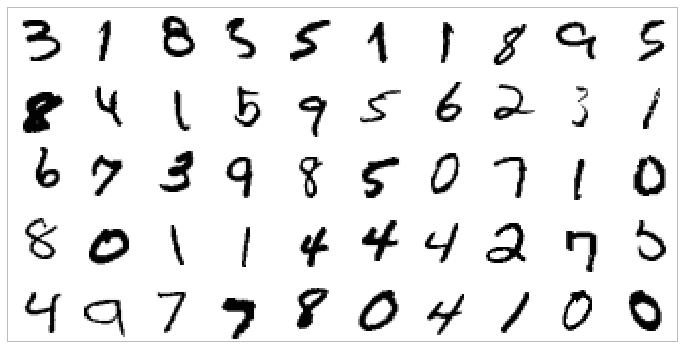
\includegraphics[scale= 0.25]{images/mnist.png}
        \caption{MNIST Data}
    \end{figure}
    \end{overlayarea}

    \column{0.6\textwidth}
    \begin{overlayarea}{\textwidth}{\textheight}

        \begin{figure}
            %
\tikzstyle{input_neuron}=[circle,draw=red!50,fill=red!10,thick,minimum size=6mm]
\tikzstyle{hidden_neuron}=[circle,draw=blue!50,fill=cyan!10,thick,minimum size=6mm]
\tikzstyle{output_neuron}=[circle,draw=green!50,fill=green!10,thick,minimum size=6mm]
\tikzstyle{cpy_neuron}=[circle,draw=green!50,fill=green!50,thick,minimum size=6mm]
\tikzstyle{input}=[circle,draw=black!50,fill=black!20,thick,minimum size=6mm]

\begin{center}
\begin{tikzpicture}

%\node [input_neuron] (neuron00) at (6.5,6) {} ;
\node [input_neuron] (neuron01) at (7.5,6) {} ;
\node [input_neuron] (neuron02) at (8.5,6)  {};
\node [input_neuron] (neuron03) at (9.5,6)  {};
\node [input_neuron] (neuron04) at (10.5,6)  {};
%\node [input_neuron] (neuron05) at (11.5,6)  {};
\node [input_neuron] (neuron06) at (12.5,6)  {};
%\node [input_neuron] (neuron07) at (13.5,6) {} ;

\node [output_neuron] (neuron11) at (7.5,7.5)  {$0$};
\node [output_neuron] (neuron12) at (8.5,7.5)  {$1$};
\node [output_neuron] (neuron13) at (9.5,7.5)  {$2$};
\node [cpy_neuron] (neuron14) at (10.5,7.5)  {$3$};
\node [output_neuron] (neuron15) at (12.5,7.5)  {$9$};


%\node[text width=0.01cm] at (12.2,4.5) {$x$};
%\node[text width=0.01cm] at (13.2,6) {$h$};
%\node[text width=0.01cm] at (12.2,7.5) {$\hat{x}$};

\draw[red!100,thick,solid,rounded corners=15pt] (7,5.5) rectangle (13,6.5);
%\draw[red!100,thick,solid,rounded corners=15pt] (8,7) rectangle (12,8);

\node[] at (10.2,5) {$|\textbf{x}_i| = 784 = 28 \times 28$};

\node[text width=0.5cm] at (10.2,4) 
 {
\includegraphics[width=.9\textwidth]{images/three.jpeg}};
\draw[black, thick] (9.7,3.5) rectangle (10.7,4.5);
\node[] at (10.2,3.2) {28*28};

\draw[->] (10.5,6.5) -- (neuron14);
\draw[->] (9.5,6.5) -- (neuron13);
\draw[->] (8.5,6.5) -- (neuron12);
\draw[->] (7.5,6.5) -- (neuron11);
\draw[->] (12.5,6.5) -- (neuron15);

\draw[red!20,dashed,line width=2pt] (neuron04) -- (neuron06);
\draw[green!20,dashed,line width=2pt] (neuron14) -- (neuron15);

\end{tikzpicture}
\end{center}
             
\tikzstyle{input_neuron}=[circle,draw=red!50,fill=red!10,thick,minimum size=6mm]
\tikzstyle{hidden_neuron}=[circle,draw=blue!50,fill=cyan!10,thick,minimum size=6mm]
\tikzstyle{output_neuron}=[circle,draw=green!50,fill=green!10,thick,minimum size=6mm]
\tikzstyle{cpy_neuron}=[circle,draw=green!50,fill=green!50,thick,minimum size=6mm]
\tikzstyle{input}=[circle,draw=black!50,fill=black!20,thick,minimum size=6mm]

\begin{center}
\begin{tikzpicture}

%\node [input_neuron] (neuron00) at (6.5,6) {} ;
\node [input_neuron] (neuron01) at (7.5,6) {} ;
\node [input_neuron] (neuron02) at (8.5,6)  {};
\node [input_neuron] (neuron03) at (9.5,6)  {};
\node [input_neuron] (neuron04) at (10.5,6)  {};
%\node [input_neuron] (neuron05) at (11.5,6)  {};
\node [input_neuron] (neuron06) at (12.5,6)  {};
%\node [input_neuron] (neuron07) at (13.5,6) {} ;

\node [output_neuron] (neuron11) at (7.5,7.5)  {$0$};
\node [output_neuron] (neuron12) at (8.5,7.5)  {$1$};
\node [output_neuron] (neuron13) at (9.5,7.5)  {$2$};
\node [cpy_neuron] (neuron14) at (10.5,7.5)  {$3$};
\node [output_neuron] (neuron15) at (12.5,7.5)  {$9$};


%\node[text width=0.01cm] at (12.2,4.5) {$x$};
%\node[text width=0.01cm] at (13.2,6) {$h$};
%\node[text width=0.01cm] at (12.2,7.5) {$\hat{x}$};

\draw[red!100,thick,solid,rounded corners=15pt] (7,5.5) rectangle (13,6.5);
%\draw[red!100,thick,solid,rounded corners=15pt] (8,7) rectangle (12,8);

\node[] at (10.2,5) {$|\textbf{x}_i| = 784 = 28 \times 28$};

\node[text width=0.5cm] at (10.2,4) 
 {
\includegraphics[width=.9\textwidth]{images/three.jpeg}};
\draw[black, thick] (9.7,3.5) rectangle (10.7,4.5);
\node[] at (10.2,3.2) {28*28};

\draw[->] (10.5,6.5) -- (neuron14);
\draw[->] (9.5,6.5) -- (neuron13);
\draw[->] (8.5,6.5) -- (neuron12);
\draw[->] (7.5,6.5) -- (neuron11);
\draw[->] (12.5,6.5) -- (neuron15);

\draw[red!20,dashed,line width=2pt] (neuron04) -- (neuron06);
\draw[green!20,dashed,line width=2pt] (neuron14) -- (neuron15);

\end{tikzpicture}
\end{center}
            \caption{Basic approach(we use raw data as input features)}
        \end{figure}

    \end{overlayarea}

  \end{columns}
\end{frame}

\begin{frame}
  \begin{columns}
    \column{0.4\textwidth}

    \begin{overlayarea}{\textwidth}{\textheight}
        \vspace{0.2in}
        \textbf{\large{Task: Hand-written digit recognition}}
        \begin{figure}
            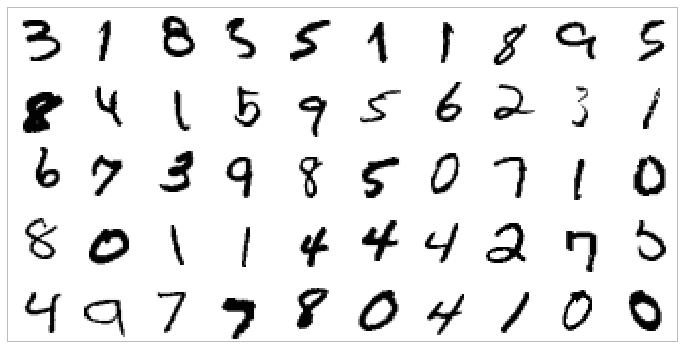
\includegraphics[scale= 0.25]{images/mnist.png}
        \caption{MNIST Data}
        \end{figure}
    \end{overlayarea}

    \column{0.6\textwidth}
    \begin{overlayarea}{\textwidth}{\textheight}
    \begin{figure}
            \hspace{2cm}
			
\begin{tikzpicture}
	\tikzstyle{input_neuron}=[circle,draw=red!50,fill=red!10,thick,minimum size=6mm]
	\tikzstyle{hidden_neuron}=[circle,draw=blue!50,fill=cyan!10,thick,minimum size=6mm]
	\tikzstyle{output_neuron}=[circle,draw=green!50,fill=green!10,thick,minimum size=6mm]
	\tikzstyle{cpy_neuron}=[circle,draw=red!50,fill=red!50,thick,minimum size=6mm]
	\tikzstyle{input}=[circle,draw=black!50,fill=black!20,thick,minimum size=6mm]

	\node [input_neuron] (neuron00) at (7.5,4.5) {};
	\node [input_neuron] (neuron01) at (8.5,4.5) {};
	\node [input_neuron] (neuron02) at (9.5,4.5){};
	\node [input_neuron] (neuron03) at (10.5,4.5) {};
	%\node [input_neuron] (neuron04) at (11.5,4.5) {};
	\node [input_neuron] (neuron05) at (12.5,4.5) {};

	%\node [hidden_neuron] (neuron51) at (7.5,6) {} ;
	\node [hidden_neuron] (neuron52) at (8.5,6)  {};
	\node [hidden_neuron] (neuron53) at (9.5,6)  {};
	%\node [hidden_neuron] (neuron54) at (10.5,6)  {};
	\node [hidden_neuron] (neuron55) at (11.5,6)  {};
	%\node [hidden_neuron] (neuron56) at (12.5,6)  {};

	\node [output_neuron] (neuron10) at (7.5,7.5)  {};
	\node [output_neuron] (neuron11) at (8.5,7.5)  {};
	\node [output_neuron] (neuron12) at (9.5,7.5)  {};
	\node [output_neuron] (neuron13) at (10.5,7.5)  {};
	%\node [output_neuron] (neuron14) at (11.5,7.5)  {};
	\node [output_neuron] (neuron14) at (12.5,7.5)  {};

	\draw[red!100,thick,solid,rounded corners=15pt] (7,4) rectangle (13,5);
	\draw[red!100,thick,solid,rounded corners=15pt] (8,5.5) rectangle (12,6.5);
	\draw[red!100,thick,solid,rounded corners=15pt] (7,7) rectangle (13,8);

	%\draw[black!50,thick,solid] (7,5) -- (8,5.5);
	%\draw[black!50,thick,solid] (13,5) -- (12,5.5);
	%\draw[black!50,thick,solid] (8,6.5) -- (7,7);
	%\draw[black!50,thick,solid] (12,6.5) -- (13,7);        
	\draw[thick,->] (10,5) -- (10,5.5);

	\draw[thick,->] (10,6.5) -- (10,7);

	%\node[] at (7.4,6) {\textbf{•}xtbf{h}};     

	\draw[red!20,dashed,line width=2pt] (neuron03) -- (neuron05);
	\draw[blue!20,dashed,line width=2pt] (neuron53) -- (neuron55);
	\draw[green!20,dashed,line width=2pt] (neuron13) -- (neuron14);        

	\node[] at (10,3.5) {$|\textbf{x}_i| = 784 = 28 \times 28$};
	\node[] at (13.9,8) {$\hat{\textbf{x}}_i \in \mathbb{R}^{784}$};
	\node[] at (13,6) {$\textbf{h} \in \mathbb{R}^{d}$};      
	\node[text width=0.5cm] at (10,2.5) 
	    {
\includegraphics[width=.9\textwidth]{images/three.jpeg}};
	\draw[black, thick] (9.5,2) rectangle (10.5,3);             
        
\end{tikzpicture}

            \vspace{0.3cm}
        \caption{\small{AE approach (first learn important characteristics of data)}} 
    \end{figure}
 
    \end{overlayarea}
  \end{columns}
\end{frame}

\begin{frame}
  \begin{columns}
    \column{0.4\textwidth}

    \begin{overlayarea}{\textwidth}{\textheight}
        \vspace{0.2in}
        \textbf{\large{Task: Hand-written digit recognition}}
        \begin{figure}
            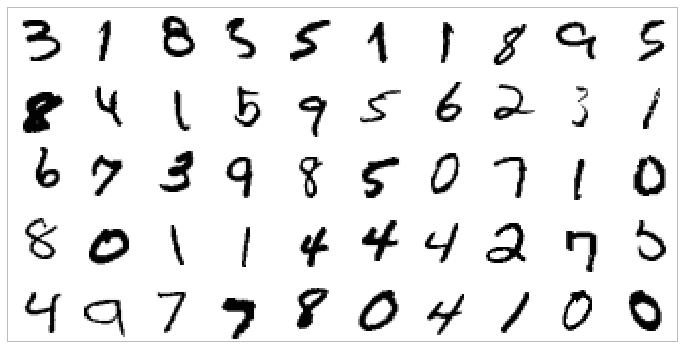
\includegraphics[scale= 0.25]{images/mnist.png}
        \caption{MNIST Data}
        \end{figure}
    \end{overlayarea}

      \column{0.6\textwidth}
      
    \begin{overlayarea}{\textwidth}{\textheight}

            \begin{figure}
        \hspace{2cm}
        %         \tikzstyle{input_neuron}=[circle,draw=red!50,fill=red!10,thick,minimum size=6mm]
		\tikzstyle{hidden_neuron}=[circle,draw=blue!50,fill=cyan!10,thick,minimum size=6mm]
		\tikzstyle{output_neuron}=[circle,draw=green!50,fill=green!10,thick,minimum size=6mm]
		\tikzstyle{cpy_neuron}=[circle,draw=red!50,fill=red!50,thick,minimum size=6mm]
		\tikzstyle{input}=[circle,draw=black!50,fill=black!20,thick,minimum size=6mm]

\begin{center}

\begin{tikzpicture}

		\node [input_neuron] (neuron00) at (7.5,4.5) {};
        \node [input_neuron] (neuron01) at (8.5,4.5) {};
		\node [input_neuron] (neuron02) at (9.5,4.5){};
		\node [input_neuron] (neuron03) at (10.5,4.5) {};
		%\node [input_neuron] (neuron04) at (11.5,4.5) {};
		\node [input_neuron] (neuron05) at (12.5,4.5) {};
		
		%\node [hidden_neuron] (neuron51) at (7.5,6) {} ;
		\node [hidden_neuron] (neuron52) at (8.5,6)  {};
		\node [hidden_neuron] (neuron53) at (9.5,6)  {};
		%\node [hidden_neuron] (neuron54) at (10.5,6)  {};
		\node [hidden_neuron] (neuron55) at (11.5,6)  {};
		%\node [hidden_neuron] (neuron56) at (12.5,6)  {};
		
		\node [output_neuron] (neuron10) at (7.5,7.5)  {$0$};
		\node [output_neuron] (neuron11) at (8.5,7.5)  {$1$};
		\node [output_neuron] (neuron12) at (9.5,7.5)  {$2$};
		\node [output_neuron] (neuron13) at (10.5,7.5)  {$3$};
		%\node [output_neuron] (neuron14) at (11.5,7.5)  {};
		\node [output_neuron] (neuron14) at (12.5,7.5)  {$9$};
		
		\draw[red!100,thick,solid,rounded corners=15pt] (7,4) rectangle (13,5);
		\draw[red!100,thick,solid,rounded corners=15pt] (8,5.5) rectangle (12,6.5);
		%\draw[red!100,thick,solid,rounded corners=15pt] (7,7) rectangle (13,8);
		
		%\draw[black!50,thick,solid] (7,5) -- (8,5.5);
		%\draw[black!50,thick,solid] (13,5) -- (12,5.5);
		%\draw[black!50,thick,solid] (8,6.5) -- (7,7);
		%\draw[black!50,thick,solid] (12,6.5) -- (13,7);		
		%\draw[thick,->] (10,5) -- (10,5.5);
		%\draw[thick,->] (10,6.5) -- (10,7);
		
		\foreach \x in {neuron10,neuron11,neuron12,neuron13,neuron14}
			\draw[thick,->] (10,6.5) -- (\x);
		
		%\node[] at (7.4,6) {\textbf{h}};		
		
		\draw[thick,->] (10,5) -- (10,5.5);
		
		
		\draw[red!20,dashed,line width=2pt] (neuron03) -- (neuron05);
		\draw[blue!20,dashed,line width=2pt] (neuron53) -- (neuron55);
		\draw[green!20,dashed,line width=2pt] (neuron13) -- (neuron14);        
		
		\node[] at (10,3.5) {$|\textbf{x}_i| = 784 = 28 \times 28$};
		%\node[] at (13.5,8) {$\hat{x} \in \mathbb{R}^{784}$};
		\node[] at (13,6) {$\textbf{h} \in \mathbb{R}^{d}$};		
		\node[text width=0.5cm] at (10,2.5) 
 			{
\includegraphics[width=.9\textwidth]{images/three.jpeg}};
		\draw[black, thick] (9.5,2) rectangle (10.5,3);				
		
\end{tikzpicture}

\end{center}
                \tikzstyle{input_neuron}=[circle,draw=red!50,fill=red!10,thick,minimum size=6mm]
		\tikzstyle{hidden_neuron}=[circle,draw=blue!50,fill=cyan!10,thick,minimum size=6mm]
		\tikzstyle{output_neuron}=[circle,draw=green!50,fill=green!10,thick,minimum size=6mm]
		\tikzstyle{cpy_neuron}=[circle,draw=red!50,fill=red!50,thick,minimum size=6mm]
		\tikzstyle{input}=[circle,draw=black!50,fill=black!20,thick,minimum size=6mm]

\begin{center}

\begin{tikzpicture}

		\node [input_neuron] (neuron00) at (7.5,4.5) {};
        \node [input_neuron] (neuron01) at (8.5,4.5) {};
		\node [input_neuron] (neuron02) at (9.5,4.5){};
		\node [input_neuron] (neuron03) at (10.5,4.5) {};
		%\node [input_neuron] (neuron04) at (11.5,4.5) {};
		\node [input_neuron] (neuron05) at (12.5,4.5) {};
		
		%\node [hidden_neuron] (neuron51) at (7.5,6) {} ;
		\node [hidden_neuron] (neuron52) at (8.5,6)  {};
		\node [hidden_neuron] (neuron53) at (9.5,6)  {};
		%\node [hidden_neuron] (neuron54) at (10.5,6)  {};
		\node [hidden_neuron] (neuron55) at (11.5,6)  {};
		%\node [hidden_neuron] (neuron56) at (12.5,6)  {};
		
		\node [output_neuron] (neuron10) at (7.5,7.5)  {$0$};
		\node [output_neuron] (neuron11) at (8.5,7.5)  {$1$};
		\node [output_neuron] (neuron12) at (9.5,7.5)  {$2$};
		\node [output_neuron] (neuron13) at (10.5,7.5)  {$3$};
		%\node [output_neuron] (neuron14) at (11.5,7.5)  {};
		\node [output_neuron] (neuron14) at (12.5,7.5)  {$9$};
		
		\draw[red!100,thick,solid,rounded corners=15pt] (7,4) rectangle (13,5);
		\draw[red!100,thick,solid,rounded corners=15pt] (8,5.5) rectangle (12,6.5);
		%\draw[red!100,thick,solid,rounded corners=15pt] (7,7) rectangle (13,8);
		
		%\draw[black!50,thick,solid] (7,5) -- (8,5.5);
		%\draw[black!50,thick,solid] (13,5) -- (12,5.5);
		%\draw[black!50,thick,solid] (8,6.5) -- (7,7);
		%\draw[black!50,thick,solid] (12,6.5) -- (13,7);		
		%\draw[thick,->] (10,5) -- (10,5.5);
		%\draw[thick,->] (10,6.5) -- (10,7);
		
		\foreach \x in {neuron10,neuron11,neuron12,neuron13,neuron14}
			\draw[thick,->] (10,6.5) -- (\x);
		
		%\node[] at (7.4,6) {\textbf{h}};		
		
		\draw[thick,->] (10,5) -- (10,5.5);
		
		
		\draw[red!20,dashed,line width=2pt] (neuron03) -- (neuron05);
		\draw[blue!20,dashed,line width=2pt] (neuron53) -- (neuron55);
		\draw[green!20,dashed,line width=2pt] (neuron13) -- (neuron14);        
		
		\node[] at (10,3.5) {$|\textbf{x}_i| = 784 = 28 \times 28$};
		%\node[] at (13.5,8) {$\hat{x} \in \mathbb{R}^{784}$};
		\node[] at (13,6) {$\textbf{h} \in \mathbb{R}^{d}$};		
		\node[text width=0.5cm] at (10,2.5) 
 			{
\includegraphics[width=.9\textwidth]{images/three.jpeg}};
		\draw[black, thick] (9.5,2) rectangle (10.5,3);				
		
\end{tikzpicture}

\end{center}
        % \vspace{-0.4in}
        \caption{\small{AE approach (and then train a classifier on top of this hidden representation) }}
    \end{figure}
   
    \end{overlayarea}
  \end{columns}
\end{frame}


\begin{frame}
    \begin{block}{}
        We will now see a way of visualizing AEs and use this visualization to compare different AEs
    \end{block}
\end{frame}

\begin{frame}
  \begin{columns}
    \column{0.4\textwidth}
    \begin{overlayarea}{\textwidth}{\textheight}
        \begin{figure}
            % \tikzstyle{input_neuron}=[circle,draw=red!50,fill=red!10,thick,minimum size=6mm]
\tikzstyle{hidden_neuron}=[circle,draw=blue!50,fill=cyan!10,thick,minimum size=6mm]
\tikzstyle{output_neuron}=[circle,draw=green!50,fill=green!10,thick,minimum size=6mm]
\tikzstyle{cpy_neuron}=[circle,draw=blue!50,fill=blue!50,thick,minimum size=6mm]
\tikzstyle{input}=[circle,draw=black!50,fill=black!20,thick,minimum size=6mm]

\begin{center}
\begin{tikzpicture}

\node [input_neuron] (neuron01) at (6.5,4.5) {};
\node [input_neuron] (neuron02) at (7.5,4.5){};
\node [input_neuron] (neuron03) at (8.5,4.5) {};
\node [input_neuron] (neuron04) at (9.5,4.5) {};
\node [input_neuron] (neuron05) at (10.5,4.5) {};
\node [cpy_neuron] (neuron51) at (7,6) {} ;
\node [hidden_neuron] (neuron52) at (8,6)  {};
\node [hidden_neuron] (neuron53) at (9,6)  {};
\node [hidden_neuron] (neuron54) at (10,6)  {};

\node [output_neuron] (neuron11) at (6.5,7.5)  {};
\node [output_neuron] (neuron12) at (7.5,7.5)  {};
\node [output_neuron] (neuron13) at (8.5,7.5)  {};
\node [output_neuron] (neuron14) at (9.5,7.5)  {};
\node [output_neuron] (neuron15) at (10.5,7.5)  {};

\node[text width=0.01cm] at (11.2,4.5) {$\textbf{x}_i$};
\node[text width=0.01cm] at (10.7,6) {$\textbf{h}$};
\node[text width=0.01cm] at (11.2,7.5) {$\hat{\textbf{x}}_i$};

%\node[] at (8.5,3.2) {AE approach};

\draw[red!100,thick,solid,rounded corners=15pt] (6,4) rectangle (11,5);
\draw[red!100,thick,solid,rounded corners=15pt] (6.5,5.5) rectangle (10.5,6.5);
\draw[red!100,thick,solid,rounded corners=15pt] (6,7) rectangle (11,8);
\draw[thick,->](neuron01) -- (neuron51);
\draw[thick,->](neuron02) -- (neuron51);
\draw[thick,->](neuron03) -- (neuron51);
\draw[thick,->](neuron04) -- (neuron51);
\draw[thick,->](neuron05) -- (neuron51);

\draw[thick,->] (8.5,5) -- (8.5,5.5);

\draw[thick,->] (8.5,6.5) -- (8.5,7);



\end{tikzpicture}
\end{center}

            \tikzstyle{input_neuron}=[circle,draw=red!50,fill=red!10,thick,minimum size=6mm]
\tikzstyle{hidden_neuron}=[circle,draw=blue!50,fill=cyan!10,thick,minimum size=6mm]
\tikzstyle{output_neuron}=[circle,draw=green!50,fill=green!10,thick,minimum size=6mm]
\tikzstyle{cpy_neuron}=[circle,draw=blue!50,fill=blue!50,thick,minimum size=6mm]
\tikzstyle{input}=[circle,draw=black!50,fill=black!20,thick,minimum size=6mm]

\begin{center}
\begin{tikzpicture}

\node [input_neuron] (neuron01) at (6.5,4.5) {};
\node [input_neuron] (neuron02) at (7.5,4.5){};
\node [input_neuron] (neuron03) at (8.5,4.5) {};
\node [input_neuron] (neuron04) at (9.5,4.5) {};
\node [input_neuron] (neuron05) at (10.5,4.5) {};
\node [cpy_neuron] (neuron51) at (7,6) {} ;
\node [hidden_neuron] (neuron52) at (8,6)  {};
\node [hidden_neuron] (neuron53) at (9,6)  {};
\node [hidden_neuron] (neuron54) at (10,6)  {};

\node [output_neuron] (neuron11) at (6.5,7.5)  {};
\node [output_neuron] (neuron12) at (7.5,7.5)  {};
\node [output_neuron] (neuron13) at (8.5,7.5)  {};
\node [output_neuron] (neuron14) at (9.5,7.5)  {};
\node [output_neuron] (neuron15) at (10.5,7.5)  {};

\node[text width=0.01cm] at (11.2,4.5) {$\textbf{x}_i$};
\node[text width=0.01cm] at (10.7,6) {$\textbf{h}$};
\node[text width=0.01cm] at (11.2,7.5) {$\hat{\textbf{x}}_i$};

%\node[] at (8.5,3.2) {AE approach};

\draw[red!100,thick,solid,rounded corners=15pt] (6,4) rectangle (11,5);
\draw[red!100,thick,solid,rounded corners=15pt] (6.5,5.5) rectangle (10.5,6.5);
\draw[red!100,thick,solid,rounded corners=15pt] (6,7) rectangle (11,8);
\draw[thick,->](neuron01) -- (neuron51);
\draw[thick,->](neuron02) -- (neuron51);
\draw[thick,->](neuron03) -- (neuron51);
\draw[thick,->](neuron04) -- (neuron51);
\draw[thick,->](neuron05) -- (neuron51);

\draw[thick,->] (8.5,5) -- (8.5,5.5);

\draw[thick,->] (8.5,6.5) -- (8.5,7);



\end{tikzpicture}
\end{center}

            % \vspace{-1.5cm}
        \end{figure}

    \footnotesize{
    \onslide<5->{
    \begin{block}{}
    \begin{align*}
        \underset{\textbf{x}_i}{\max} \hspace{0.1in} & \{W_{1}^{T}\textbf{x}_{i}\}\\
         s.t.\hspace{0.1in}  ||\textbf{x}_{i}||^{2} &= \textbf{x}_{i}^{T}\textbf{x}_{i} = 1\\
        \onslide<6->{\text{Solution:}\hspace{0.1in}  \textbf{x}_{i} &= \frac{W_{1}}{\sqrt{W_1^TW_1}}}                             
    \end{align*}
    \end{block}}}


    %$\underset{x}{\arg \max} ~ W^{T}*x ~ s.t. ~ \|{x}\|^2  =  x^T*x = 1$ \\

    %$Solution: x = \frac{W_{1}}{\sqrt{W_1^{T}W_{1}}}$

    \end{overlayarea}

    \column{0.6\textwidth}
    \begin{overlayarea}{\textwidth}{\textheight}
        \only <1-> {
            \begin{itemize}\justifying
                  \item <1-> We can think of each neuron as a filter which will fire (or get maximally) activated for a certain input configuration $\textbf{x}_{i}$ 
                  \item <2-> For example, \\
                     \[\textbf{h}_{1} = \sigma(W_{1}^{T}\textbf{x}_{i}) ~ [ignoring ~ bias ~ b]\]
                     Where $W_{1}$ is the trained vector of weights connecting the input to the first hidden neuron 
                  \item <3-> What values of $\textbf{x}_i$ will cause $\textbf{h}_1$ to be maximum (or maximally activated)
                  \item <4-> Suppose we assume that our inputs are normalized so that $\|{\textbf{x}_i}\| = 1$      
            \end{itemize}
        }
    \end{overlayarea}
  \end{columns}
\end{frame}


\begin{frame}
  \begin{columns}
    \column{0.4\textwidth}
    \begin{overlayarea}{\textwidth}{\textheight}
        \begin{figure}
            % \tikzstyle{input_neuron}=[circle,draw=red!50,fill=red!10,thick,minimum size=6mm]
\tikzstyle{hidden_neuron}=[circle,draw=blue!50,fill=cyan!10,thick,minimum size=6mm]
\tikzstyle{output_neuron}=[circle,draw=green!50,fill=green!10,thick,minimum size=6mm]
\tikzstyle{cpy_neuron}=[circle,draw=blue!50,fill=blue!50,thick,minimum size=6mm]
\tikzstyle{input}=[circle,draw=black!50,fill=black!20,thick,minimum size=6mm]

\begin{center}
\begin{tikzpicture}

\node [input_neuron] (neuron01) at (6.5,4.5) {};
\node [input_neuron] (neuron02) at (7.5,4.5){};
\node [input_neuron] (neuron03) at (8.5,4.5) {};
\node [input_neuron] (neuron04) at (9.5,4.5) {};
\node [input_neuron] (neuron05) at (10.5,4.5) {};
\node [cpy_neuron] (neuron51) at (7,6) {} ;
\node [hidden_neuron] (neuron52) at (8,6)  {};
\node [hidden_neuron] (neuron53) at (9,6)  {};
\node [hidden_neuron] (neuron54) at (10,6)  {};

\node [output_neuron] (neuron11) at (6.5,7.5)  {};
\node [output_neuron] (neuron12) at (7.5,7.5)  {};
\node [output_neuron] (neuron13) at (8.5,7.5)  {};
\node [output_neuron] (neuron14) at (9.5,7.5)  {};
\node [output_neuron] (neuron15) at (10.5,7.5)  {};

\node[text width=0.01cm] at (11.2,4.5) {$\textbf{x}_i$};
\node[text width=0.01cm] at (10.7,6) {$\textbf{h}$};
\node[text width=0.01cm] at (11.2,7.5) {$\hat{\textbf{x}}_i$};

%\node[] at (8.5,3.2) {AE approach};

\draw[red!100,thick,solid,rounded corners=15pt] (6,4) rectangle (11,5);
\draw[red!100,thick,solid,rounded corners=15pt] (6.5,5.5) rectangle (10.5,6.5);
\draw[red!100,thick,solid,rounded corners=15pt] (6,7) rectangle (11,8);
\draw[thick,->](neuron01) -- (neuron51);
\draw[thick,->](neuron02) -- (neuron51);
\draw[thick,->](neuron03) -- (neuron51);
\draw[thick,->](neuron04) -- (neuron51);
\draw[thick,->](neuron05) -- (neuron51);

\draw[thick,->] (8.5,5) -- (8.5,5.5);

\draw[thick,->] (8.5,6.5) -- (8.5,7);



\end{tikzpicture}
\end{center}

            \tikzstyle{input_neuron}=[circle,draw=red!50,fill=red!10,thick,minimum size=6mm]
\tikzstyle{hidden_neuron}=[circle,draw=blue!50,fill=cyan!10,thick,minimum size=6mm]
\tikzstyle{output_neuron}=[circle,draw=green!50,fill=green!10,thick,minimum size=6mm]
\tikzstyle{cpy_neuron}=[circle,draw=blue!50,fill=blue!50,thick,minimum size=6mm]
\tikzstyle{input}=[circle,draw=black!50,fill=black!20,thick,minimum size=6mm]

\begin{center}
\begin{tikzpicture}

\node [input_neuron] (neuron01) at (6.5,4.5) {};
\node [input_neuron] (neuron02) at (7.5,4.5){};
\node [input_neuron] (neuron03) at (8.5,4.5) {};
\node [input_neuron] (neuron04) at (9.5,4.5) {};
\node [input_neuron] (neuron05) at (10.5,4.5) {};
\node [cpy_neuron] (neuron51) at (7,6) {} ;
\node [hidden_neuron] (neuron52) at (8,6)  {};
\node [hidden_neuron] (neuron53) at (9,6)  {};
\node [hidden_neuron] (neuron54) at (10,6)  {};

\node [output_neuron] (neuron11) at (6.5,7.5)  {};
\node [output_neuron] (neuron12) at (7.5,7.5)  {};
\node [output_neuron] (neuron13) at (8.5,7.5)  {};
\node [output_neuron] (neuron14) at (9.5,7.5)  {};
\node [output_neuron] (neuron15) at (10.5,7.5)  {};

\node[text width=0.01cm] at (11.2,4.5) {$\textbf{x}_i$};
\node[text width=0.01cm] at (10.7,6) {$\textbf{h}$};
\node[text width=0.01cm] at (11.2,7.5) {$\hat{\textbf{x}}_i$};

%\node[] at (8.5,3.2) {AE approach};

\draw[red!100,thick,solid,rounded corners=15pt] (6,4) rectangle (11,5);
\draw[red!100,thick,solid,rounded corners=15pt] (6.5,5.5) rectangle (10.5,6.5);
\draw[red!100,thick,solid,rounded corners=15pt] (6,7) rectangle (11,8);
\draw[thick,->](neuron01) -- (neuron51);
\draw[thick,->](neuron02) -- (neuron51);
\draw[thick,->](neuron03) -- (neuron51);
\draw[thick,->](neuron04) -- (neuron51);
\draw[thick,->](neuron05) -- (neuron51);

\draw[thick,->] (8.5,5) -- (8.5,5.5);

\draw[thick,->] (8.5,6.5) -- (8.5,7);



\end{tikzpicture}
\end{center}

            % \vspace{-1.5cm}
        \end{figure}

    \footnotesize{
    \begin{block}{}
    \begin{align*}
        \underset{\textbf{x}_i}{\max} \hspace{0.1in} & \{W_{1}^{T}\textbf{x}_{i}\}\\
         s.t.\hspace{0.1in}  ||\textbf{x}_i ||^{2} &= \textbf{x}_{i}^{T}\textbf{x}_{i} = 1\\
        \text{Solution:}\hspace{0.1in}  \textbf{x}_{i} &= \frac{W_{1}}{\sqrt{W_1^TW_1}}                               
    \end{align*}
    \end{block}}
    \end{overlayarea}

    \column{0.6\textwidth}
    \begin{overlayarea}{\textwidth}{\textheight}
        \begin{itemize}\justifying
            \item<1-> Thus the inputs \\
             \[ \textbf{x}_{i} =  \frac{W_{1}}{\sqrt{W_1^{T}W_{1}}}, \frac{W_{2}}{\sqrt{W_2^{T}W_{2}}}, \dots \frac{W_{n}}{\sqrt{W_n^{T}W_{n}}}  \]
            will respectively cause hidden neurons $1$ to $n$ to maximally fire    
        
            \item<2-> Let us plot these images ($\textbf{x}_{i}$'s) which maximally activate the first $k$ neurons  of the hidden representations learned by a vanilla autoencoder and different denoising autoencoders
   
            \item<3-> These $\textbf{x}_{i}$'s are computed by the above formula using the weights $(W_{1}, W_{2} \dots W_{k})$ learned by the respective autoencoders
        \end{itemize}
    \end{overlayarea}
  \end{columns}
\end{frame}

\begin{frame}
    \begin{figure}
    \minipage{0.25\textwidth}
        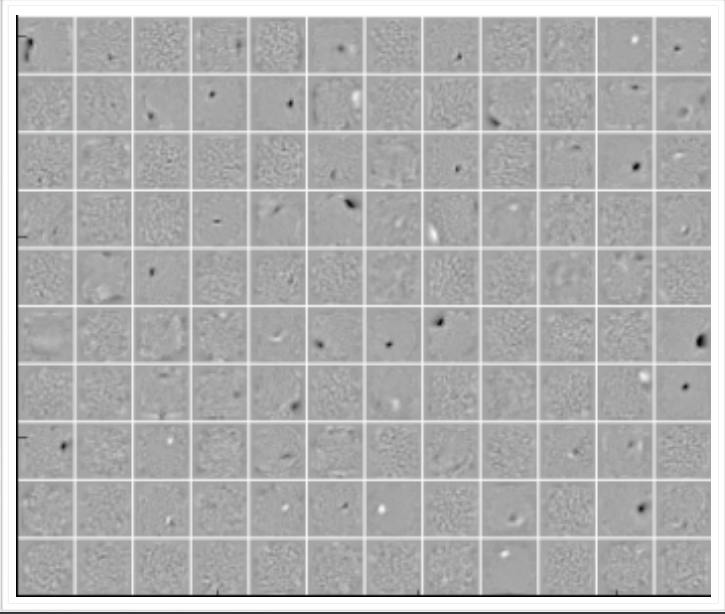
\includegraphics[width=\linewidth,height=3cm]{images/cross-entropy-loss.png}
        \label{fig:awesome_image1}
        \caption{Vanilla AE (No noise)}
    \endminipage\hfill
    \minipage{0.25\textwidth}
        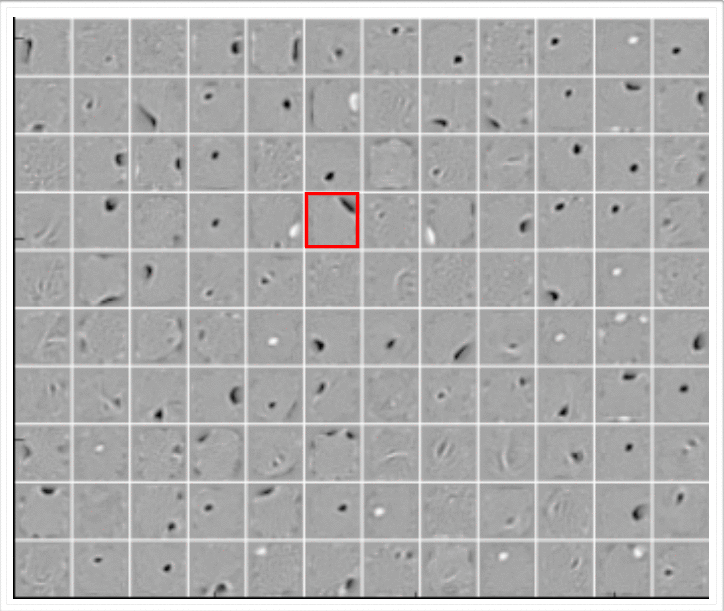
\includegraphics[width=\linewidth, height=3cm]{images/25_edited2.png}
        \label{fig:awesome_image2}
        \caption{25\% Denoising AE (q=0.25)}
    \endminipage\hfill
    \minipage{0.25\textwidth}%
        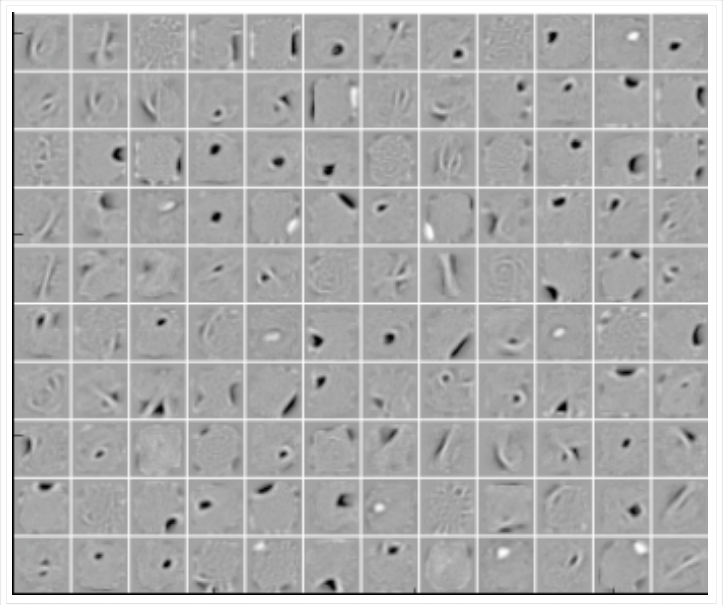
\includegraphics[width=\linewidth,height=3cm]{images/50.png}
        \label{fig:awesome_image3}
        \caption{50\% Denoising AE (q=0.5)}
    \endminipage
    \end{figure}

    \begin{itemize}\justifying
        \item<1-> The vanilla AE does not learn many meaningful patterns
        \item<2-> The hidden neurons of the denoising AEs seem to act like pen-stroke detectors (for example, in the highlighted neuron the black region is a stroke that you would expect in a '0' or a '2' or a '3' or a '8' or a '9')  
        \item<3-> As the noise increases the filters become more wide because the neuron has to rely on more adjacent pixels to feel confident about a stroke
    \end{itemize}
\end{frame}

\begin{frame}

  \begin{columns}
    \column{0.4\textwidth}
        \begin{overlayarea}{\textwidth}{\textheight}
            % \tikzstyle{input_neuron}=[circle,draw=red!50,fill=red!10,thick,minimum size=6mm]
\tikzstyle{hidden_neuron}=[circle,draw=blue!50,fill=cyan!10,thick,minimum size=6mm]
\tikzstyle{output_neuron}=[circle,draw=green!50,fill=green!10,thick,minimum size=6mm]
\tikzstyle{cpy_neuron}=[circle,draw=red!50,fill=red!50,thick,minimum size=6mm]
\tikzstyle{input}=[circle,draw=black!50,fill=black!20,thick,minimum size=6mm]

\begin{center}
\begin{tikzpicture}

\node [input_neuron] (neuron001) at (8.5,3) {};
\node [input_neuron] (neuron002) at (9.5,3){};
\node [input_neuron] (neuron003) at (10.5,3) {};
\node [input_neuron] (neuron004) at (11.5,3) {};

\node [input_neuron] (neuron01) at (8.5,4.5) {};
\node [cpy_neuron] (neuron02) at (9.5,4.5){};
\node [cpy_neuron] (neuron03) at (10.5,4.5) {};
\node [input_neuron] (neuron04) at (11.5,4.5) {};

\node [hidden_neuron] (neuron51) at (7.5,6) {} ;
\node [hidden_neuron] (neuron52) at (8.5,6)  {};
\node [hidden_neuron] (neuron53) at (9.5,6)  {};
\node [hidden_neuron] (neuron54) at (10.5,6)  {};
\node [hidden_neuron] (neuron55) at (11.5,6)  {};
\node [hidden_neuron] (neuron56) at (12.5,6)  {};

\node [output_neuron] (neuron11) at (8.5,7.5)  {};
\node [output_neuron] (neuron12) at (9.5,7.5)  {};
\node [output_neuron] (neuron13) at (10.5,7.5)  {};
\node [output_neuron] (neuron14) at (11.5,7.5)  {};

\node[text width=0.01cm] at (12.2,3) {$\mathbf{\textbf{x}_i}$};
\node[text width=0.01cm] at (12.2,4.5) {$\mathbf{\tilde{\textbf{x}}_i}$};
\node[text width=0.01cm] at (13.2,6) {$\mathbf{h}$};
\node[text width=0.01cm] at (12.2,7.5) {$\mathbf{\hat{x}_{i}}$};

\draw[red!100,thick,solid,rounded corners=15pt] (8,2.5) rectangle (12,3.5);
\draw[red!100,thick,solid,rounded corners=15pt] (8,4) rectangle (12,5);
\draw[red!100,thick,solid,rounded corners=15pt] (7,5.5) rectangle (13,6.5);
\draw[red!100,thick,solid,rounded corners=15pt] (8,7) rectangle (12,8);

\draw[thick,->] (10,3.5) -- (10,4) node [pos=0.5,right] {$P(\widetilde{x}_{ij}|x_{ij})$};

\draw[thick,->] (10,5) -- (10,5.5);

\draw[thick,->] (10,6.5) -- (10,7);

\end{tikzpicture}
\end{center}
            \tikzstyle{input_neuron}=[circle,draw=red!50,fill=red!10,thick,minimum size=6mm]
\tikzstyle{hidden_neuron}=[circle,draw=blue!50,fill=cyan!10,thick,minimum size=6mm]
\tikzstyle{output_neuron}=[circle,draw=green!50,fill=green!10,thick,minimum size=6mm]
\tikzstyle{cpy_neuron}=[circle,draw=red!50,fill=red!50,thick,minimum size=6mm]
\tikzstyle{input}=[circle,draw=black!50,fill=black!20,thick,minimum size=6mm]

\begin{center}
\begin{tikzpicture}

\node [input_neuron] (neuron001) at (8.5,3) {};
\node [input_neuron] (neuron002) at (9.5,3){};
\node [input_neuron] (neuron003) at (10.5,3) {};
\node [input_neuron] (neuron004) at (11.5,3) {};

\node [input_neuron] (neuron01) at (8.5,4.5) {};
\node [cpy_neuron] (neuron02) at (9.5,4.5){};
\node [cpy_neuron] (neuron03) at (10.5,4.5) {};
\node [input_neuron] (neuron04) at (11.5,4.5) {};

\node [hidden_neuron] (neuron51) at (7.5,6) {} ;
\node [hidden_neuron] (neuron52) at (8.5,6)  {};
\node [hidden_neuron] (neuron53) at (9.5,6)  {};
\node [hidden_neuron] (neuron54) at (10.5,6)  {};
\node [hidden_neuron] (neuron55) at (11.5,6)  {};
\node [hidden_neuron] (neuron56) at (12.5,6)  {};

\node [output_neuron] (neuron11) at (8.5,7.5)  {};
\node [output_neuron] (neuron12) at (9.5,7.5)  {};
\node [output_neuron] (neuron13) at (10.5,7.5)  {};
\node [output_neuron] (neuron14) at (11.5,7.5)  {};

\node[text width=0.01cm] at (12.2,3) {$\mathbf{\textbf{x}_i}$};
\node[text width=0.01cm] at (12.2,4.5) {$\mathbf{\tilde{\textbf{x}}_i}$};
\node[text width=0.01cm] at (13.2,6) {$\mathbf{h}$};
\node[text width=0.01cm] at (12.2,7.5) {$\mathbf{\hat{x}_{i}}$};

\draw[red!100,thick,solid,rounded corners=15pt] (8,2.5) rectangle (12,3.5);
\draw[red!100,thick,solid,rounded corners=15pt] (8,4) rectangle (12,5);
\draw[red!100,thick,solid,rounded corners=15pt] (7,5.5) rectangle (13,6.5);
\draw[red!100,thick,solid,rounded corners=15pt] (8,7) rectangle (12,8);

\draw[thick,->] (10,3.5) -- (10,4) node [pos=0.5,right] {$P(\widetilde{x}_{ij}|x_{ij})$};

\draw[thick,->] (10,5) -- (10,5.5);

\draw[thick,->] (10,6.5) -- (10,7);

\end{tikzpicture}
\end{center}
        \end{overlayarea}

    \column{0.6\textwidth}
    \begin{overlayarea}{\textwidth}{\textheight}
        \begin{itemize}\justifying
            \item<1-> We saw one form of $P(\widetilde{x}_{ij} | x_{ij})$ which flips a fraction $q$ of the inputs to zero
            \item<2-> Another way of corrupting the inputs is to add a Gaussian noise to the input \\
            \[\widetilde{x}_{ij} = x_{ij} + \mathscr{N}(0,1)\]
            \item<3-> We will now use such a denoising AE on a different dataset and see their performance
        \end{itemize}
    \end{overlayarea}
  \end{columns}
\end{frame}

\begin{frame}
    \begin{figure}
    \minipage{0.25\textwidth}
        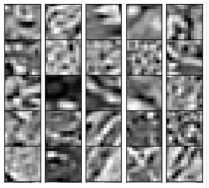
\includegraphics[width=\linewidth]{images/data.png}
        \label{fig:awesome_image1}
        \caption{Data}
    \endminipage\hfill
    \minipage{0.25\textwidth}
        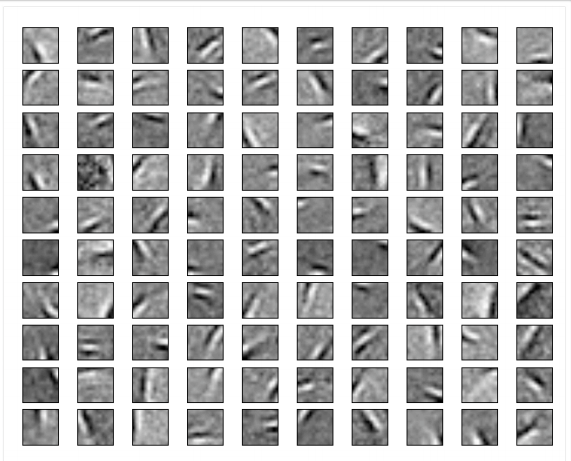
\includegraphics[width=\linewidth]{images/ae-filters.png}
        \label{fig:awesome_image2}
        \caption{AE filters}
    \endminipage\hfill
    \minipage{0.25\textwidth}%
        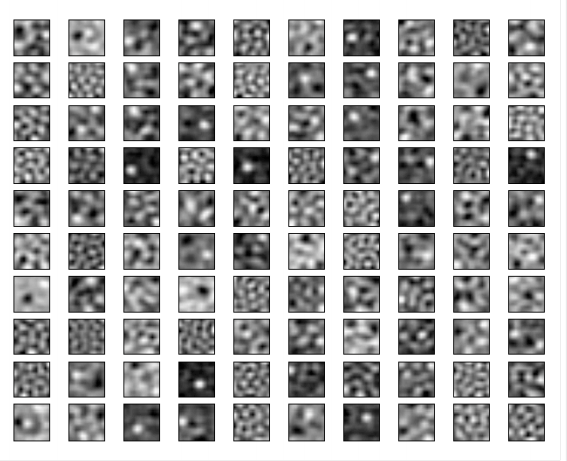
\includegraphics[width=\linewidth]{images/weight-decay.png}
        \label{fig:awesome_image3}
        \caption{Weight decay filters}
    \endminipage
    \label{pics:blablabla}
    \end{figure}

    \begin{itemize}\justifying
        \item<1-> The hidden neurons essentially behave like edge detectors
        \item<2-> PCA does not give such edge detectors
        % \item<3-> Also note that even though the noise process (adding Gaussian noise) is similar to weight decay penalty the results are very different (in particular with weight decay we do not see any meaningful patterns)   
    \end{itemize}
\end{frame}

% Slide 39 Module 4 ends


% Module 5: Sparse autoencoders (Slide 41 to 44)

\begin{frame}
    \myheading{Module 7.5: Sparse Autoencoders }
\end{frame}

\begin{frame}
  \begin{columns}
    \column{0.4\textwidth}
    \begin{overlayarea}{\textwidth}{\textheight}
        \vspace{-0.2cm}
        % \tikzstyle{input_neuron}=[circle,draw=red!50,fill=red!10,thick,minimum size=6mm]
\tikzstyle{hidden_neuron}=[circle,draw=blue!50,fill=cyan!10,thick,minimum size=6mm]
\tikzstyle{output_neuron}=[circle,draw=green!50,fill=green!10,thick,minimum size=6mm]
\tikzstyle{cpy_neuron}=[circle,draw=red!50,fill=red!50,thick,minimum size=6mm]
\tikzstyle{input}=[circle,draw=black!50,fill=black!20,thick,minimum size=6mm]

\begin{center}
\begin{tikzpicture}

\node [input_neuron] (neuron01) at (8.5,4.5) {};
\node [input_neuron] (neuron02) at (9.5,4.5){};
\node [input_neuron] (neuron03) at (10.5,4.5) {};
\node [input_neuron] (neuron04) at (11.5,4.5) {};
\node [hidden_neuron] (neuron51) at (7.5,6) {} ;
\node [hidden_neuron] (neuron52) at (8.5,6)  {};
\node [hidden_neuron] (neuron53) at (9.5,6)  {};
\node [hidden_neuron] (neuron54) at (10.5,6)  {};
\node [hidden_neuron] (neuron55) at (11.5,6)  {};
\node [hidden_neuron] (neuron56) at (12.5,6)  {};

\node [output_neuron] (neuron11) at (8.5,7.5)  {};
\node [output_neuron] (neuron12) at (9.5,7.5)  {};
\node [output_neuron] (neuron13) at (10.5,7.5)  {};
\node [output_neuron] (neuron14) at (11.5,7.5)  {};


\node[text width=0.01cm] at (12.2,4.5) {$\textbf{x}$};
\node[text width=0.01cm] at (13.2,6) {$\textbf{h}$};
\node[text width=0.01cm] at (12.2,7.5) {$\hat{\textbf{x}}$};

\draw[red!100,thick,solid,rounded corners=15pt] (8,4) rectangle (12,5);
\draw[red!100,thick,solid,rounded corners=15pt] (7,5.5) rectangle (13,6.5);
\draw[red!100,thick,solid,rounded corners=15pt] (8,7) rectangle (12,8);


\draw[thick,->] (10,5) -- (10,5.5);

\draw[thick,->] (10,6.5) -- (10,7);

\end{tikzpicture}
\end{center}
        \tikzstyle{input_neuron}=[circle,draw=red!50,fill=red!10,thick,minimum size=6mm]
\tikzstyle{hidden_neuron}=[circle,draw=blue!50,fill=cyan!10,thick,minimum size=6mm]
\tikzstyle{output_neuron}=[circle,draw=green!50,fill=green!10,thick,minimum size=6mm]
\tikzstyle{cpy_neuron}=[circle,draw=red!50,fill=red!50,thick,minimum size=6mm]
\tikzstyle{input}=[circle,draw=black!50,fill=black!20,thick,minimum size=6mm]

\begin{center}
\begin{tikzpicture}

\node [input_neuron] (neuron01) at (8.5,4.5) {};
\node [input_neuron] (neuron02) at (9.5,4.5){};
\node [input_neuron] (neuron03) at (10.5,4.5) {};
\node [input_neuron] (neuron04) at (11.5,4.5) {};
\node [hidden_neuron] (neuron51) at (7.5,6) {} ;
\node [hidden_neuron] (neuron52) at (8.5,6)  {};
\node [hidden_neuron] (neuron53) at (9.5,6)  {};
\node [hidden_neuron] (neuron54) at (10.5,6)  {};
\node [hidden_neuron] (neuron55) at (11.5,6)  {};
\node [hidden_neuron] (neuron56) at (12.5,6)  {};

\node [output_neuron] (neuron11) at (8.5,7.5)  {};
\node [output_neuron] (neuron12) at (9.5,7.5)  {};
\node [output_neuron] (neuron13) at (10.5,7.5)  {};
\node [output_neuron] (neuron14) at (11.5,7.5)  {};


\node[text width=0.01cm] at (12.2,4.5) {$\textbf{x}$};
\node[text width=0.01cm] at (13.2,6) {$\textbf{h}$};
\node[text width=0.01cm] at (12.2,7.5) {$\hat{\textbf{x}}$};

\draw[red!100,thick,solid,rounded corners=15pt] (8,4) rectangle (12,5);
\draw[red!100,thick,solid,rounded corners=15pt] (7,5.5) rectangle (13,6.5);
\draw[red!100,thick,solid,rounded corners=15pt] (8,7) rectangle (12,8);


\draw[thick,->] (10,5) -- (10,5.5);

\draw[thick,->] (10,6.5) -- (10,7);

\end{tikzpicture}
\end{center}
        % The average value of the activation of a neuron $l$ is given by
        % \[ 
        %     \hat{\rho_l} = \frac{1}{m}\sum_{i=1}^m h(\textbf{x}_i)_l
        % \]
    \end{overlayarea}

    \column{0.6\textwidth}
    \begin{overlayarea}{\textwidth}{\textheight}
        \begin{itemize}\justifying
            \item<2-> A hidden neuron with sigmoid activation will have values between 0 and 1
            \item<3->We say that the neuron is activated when its output is close to 1  and not activated when its output is close to 0.  
            \item<4-> A sparse autoencoder tries to ensure the neuron is inactive most of the times.
        \end{itemize}
    \end{overlayarea}
  \end{columns}
\end{frame}

\begin{frame}
  \begin{columns}
    \column{0.4\textwidth}
    \begin{overlayarea}{\textwidth}{\textheight}
        \vspace{-0.2cm}
        % \tikzstyle{input_neuron}=[circle,draw=red!50,fill=red!10,thick,minimum size=6mm]
\tikzstyle{hidden_neuron}=[circle,draw=blue!50,fill=cyan!10,thick,minimum size=6mm]
\tikzstyle{output_neuron}=[circle,draw=green!50,fill=green!10,thick,minimum size=6mm]
\tikzstyle{cpy_neuron}=[circle,draw=red!50,fill=red!50,thick,minimum size=6mm]
\tikzstyle{input}=[circle,draw=black!50,fill=black!20,thick,minimum size=6mm]

\begin{center}
\begin{tikzpicture}

\node [input_neuron] (neuron01) at (8.5,4.5) {};
\node [input_neuron] (neuron02) at (9.5,4.5){};
\node [input_neuron] (neuron03) at (10.5,4.5) {};
\node [input_neuron] (neuron04) at (11.5,4.5) {};
\node [hidden_neuron] (neuron51) at (7.5,6) {} ;
\node [hidden_neuron] (neuron52) at (8.5,6)  {};
\node [hidden_neuron] (neuron53) at (9.5,6)  {};
\node [hidden_neuron] (neuron54) at (10.5,6)  {};
\node [hidden_neuron] (neuron55) at (11.5,6)  {};
\node [hidden_neuron] (neuron56) at (12.5,6)  {};

\node [output_neuron] (neuron11) at (8.5,7.5)  {};
\node [output_neuron] (neuron12) at (9.5,7.5)  {};
\node [output_neuron] (neuron13) at (10.5,7.5)  {};
\node [output_neuron] (neuron14) at (11.5,7.5)  {};


\node[text width=0.01cm] at (12.2,4.5) {$\textbf{x}$};
\node[text width=0.01cm] at (13.2,6) {$\textbf{h}$};
\node[text width=0.01cm] at (12.2,7.5) {$\hat{\textbf{x}}$};

\draw[red!100,thick,solid,rounded corners=15pt] (8,4) rectangle (12,5);
\draw[red!100,thick,solid,rounded corners=15pt] (7,5.5) rectangle (13,6.5);
\draw[red!100,thick,solid,rounded corners=15pt] (8,7) rectangle (12,8);


\draw[thick,->] (10,5) -- (10,5.5);

\draw[thick,->] (10,6.5) -- (10,7);

\end{tikzpicture}
\end{center}
        \tikzstyle{input_neuron}=[circle,draw=red!50,fill=red!10,thick,minimum size=6mm]
\tikzstyle{hidden_neuron}=[circle,draw=blue!50,fill=cyan!10,thick,minimum size=6mm]
\tikzstyle{output_neuron}=[circle,draw=green!50,fill=green!10,thick,minimum size=6mm]
\tikzstyle{cpy_neuron}=[circle,draw=red!50,fill=red!50,thick,minimum size=6mm]
\tikzstyle{input}=[circle,draw=black!50,fill=black!20,thick,minimum size=6mm]

\begin{center}
\begin{tikzpicture}

\node [input_neuron] (neuron01) at (8.5,4.5) {};
\node [input_neuron] (neuron02) at (9.5,4.5){};
\node [input_neuron] (neuron03) at (10.5,4.5) {};
\node [input_neuron] (neuron04) at (11.5,4.5) {};
\node [hidden_neuron] (neuron51) at (7.5,6) {} ;
\node [hidden_neuron] (neuron52) at (8.5,6)  {};
\node [hidden_neuron] (neuron53) at (9.5,6)  {};
\node [hidden_neuron] (neuron54) at (10.5,6)  {};
\node [hidden_neuron] (neuron55) at (11.5,6)  {};
\node [hidden_neuron] (neuron56) at (12.5,6)  {};

\node [output_neuron] (neuron11) at (8.5,7.5)  {};
\node [output_neuron] (neuron12) at (9.5,7.5)  {};
\node [output_neuron] (neuron13) at (10.5,7.5)  {};
\node [output_neuron] (neuron14) at (11.5,7.5)  {};


\node[text width=0.01cm] at (12.2,4.5) {$\textbf{x}$};
\node[text width=0.01cm] at (13.2,6) {$\textbf{h}$};
\node[text width=0.01cm] at (12.2,7.5) {$\hat{\textbf{x}}$};

\draw[red!100,thick,solid,rounded corners=15pt] (8,4) rectangle (12,5);
\draw[red!100,thick,solid,rounded corners=15pt] (7,5.5) rectangle (13,6.5);
\draw[red!100,thick,solid,rounded corners=15pt] (8,7) rectangle (12,8);


\draw[thick,->] (10,5) -- (10,5.5);

\draw[thick,->] (10,6.5) -- (10,7);

\end{tikzpicture}
\end{center}
        The average value of the activation of a neuron $l$ is given by
        \[ 
            \hat{\rho}_l = \frac{1}{m}\sum_{i=1}^m h(\textbf{x}_i)_l
        \]
        %\end{onlyenv}
    \end{overlayarea}

    \column{0.6\textwidth}
    \begin{overlayarea}{\textwidth}{\textheight}
        \begin{itemize}\justifying
            \item<1-> If the neuron $l$ is sparse (i.e. mostly inactive) then $\hat{\rho}_{l} \rightarrow 0$
            \item<2->A sparse autoencoder uses  a sparsity parameter $\rho$ (typically very close to 0, say, 0.005) and tries to enforce the constraint $\hat{\rho}_{l} = \rho$
            \item<3-> One way of ensuring this is to add the following term to the objective function\\
                \[
                    \Omega(\theta) = 
                        \sum_{l=1}^k \rho \log \frac{\rho}{\hat{\rho}_l} + 
                        (1-\rho) \log \frac{1-\rho}{1-\hat{\rho}_{l}}
                \]
            \item<4->When will this term reach its minimum value and what is the minimum value? Let us plot it and check.
        \end{itemize}
    \end{overlayarea}
  \end{columns}
\end{frame}

\begin{frame}
	
\begin{tikzpicture}
	\begin{scope}[every node/.style={sloped,allow upside down}]
		\draw (1.5,3) circle (0.5em);
		\draw (0,2) circle (0.5em)
		node[below=0.15] {\tiny $x_1 + \varepsilon_1$};
		\draw (1,2) circle (0.5em)
		node[below=0.15] {\tiny $x_2 + \varepsilon_2$}
		node[right=0.19] {\dots};
		\draw (2.2,2) circle (0.5em)
		node[below=0.15] {\tiny $x_k + \varepsilon_k$}
		node[right=0.19] {\dots};
		\draw (3.4,2) circle (0.5em) node[below=0.15] {\tiny $x_n + \varepsilon_n$};
		\draw[->] (0.12,2.15) -- (1.35,2.85);
		\draw[->] (1.04,2.17) -- (1.45,2.8);
		\draw[->] (2.12,2.17) -- (1.55,2.8);
		\draw[->] (3.28,2.15) -- (1.65,2.85);
	\end{scope}
\end{tikzpicture}

    \begin{itemize}\justifying
        \item<2-> The function will reach its minimum value(s) when $\hat{\rho}_{l} = \rho$.
    
\end{itemize}
%}
%\end{overlayarea}
%\end{columns}
\end{frame}

\begin{frame}
  \begin{columns}
    \column{0.55\textwidth}
    \begin{overlayarea}{\textwidth}{\textheight}
        %\begin{itemize}
            \footnotesize{
            \onslide<5-> 
            \[ 
                \Omega(\theta) = \sum_{l=1}^k \rho log \frac{\rho}{\hat{\rho}_{l}} + (1-\rho)log\frac{1-\rho}{1-\hat{\rho}_{l}}
            \]
            \onslide<6-> Can be re-written as
            \[
                \Omega(\theta) = \sum_{l=1}^k \rho log \rho - \rho log \hat{\rho}_{l} + (1-\rho) log (1-\rho) - (1-\rho) log (1-\hat{\rho}_{l})
            \]
            \onslide<7-> By Chain rule:
            \[
                \frac{\partial{\Omega(\theta)}}{\partial{W}} = \frac{\partial{\Omega(\theta)}}{\partial{\mathbf{\hat{\rho}}}}.\frac{\partial{\mathbf{\hat{\rho}}}}{\partial{W}}
            \]
            \onslide<8-> 
            {\[
	          	 \frac{\partial{\Omega(\theta)}}{\partial{\mathbf{\hat{\rho}}}} = \begin{bmatrix}
	          	  \frac{\partial{\Omega(\theta)}}{\partial{\hat{\rho}_1}} , \frac{\partial{\Omega(\theta)}}{\partial{\hat{\rho}_2}} ,\dots  \frac{\partial{\Omega(\theta)}}{\partial{\hat{\rho}_k}} 
	          	 \end{bmatrix}^T
	         \]}
	         \onslide<9->{          
            For each neuron $l \in 1 \dots k$ in hidden layer, we have
\vspace{-0.5cm}}
	         
	         \begin{align*}
	           \onslide<10->{\frac{\partial{\Omega(\theta)}}{\partial{\hat{\rho}_l}} &= -\frac{\rho}{\hat{\rho}_l} + \frac{(1-\rho)}{1-\hat{\rho}_l}\\}
	           \onslide<11->{\text{and}\qquad
                 	\frac{\partial{\hat{\rho}_{l}}}{\partial{W}} &= \textbf{x}_{i}(g'(W^{T}\textbf{x}_{i} + \mathbf{b}))^{T} \text{(see next slide)}}
	         \end{align*}
              
            
            
            }
        %\end{itemize}
    \end{overlayarea}

    \column{0.45\textwidth}
    \small
    \begin{overlayarea}{\textwidth}{\textheight}
        \begin{itemize}\justifying
            \onslide<1-> \item Now,
                \[
                    \hat{\mathscr{L}}(\theta) = \mathscr{L}(\theta) + \Omega(\theta)
                \]
            \vspace{-0.5cm}
            \onslide<2-> \item $\mathscr{L}(\theta)$ is the squared error loss or cross entropy loss and $\Omega(\theta)$ is the      sparsity    constraint.
            \onslide<3-> \item We already know how to calculate $\frac{\partial\mathscr{L}(\theta)}{\partial W}$
            \onslide<4-> \item Let us see how to calculate $\frac{\partial{\Omega(\theta)}}{\partial{W}}$.
            \onslide<12->\item Finally,
            \[
                \frac{\partial{\hat{\mathscr{L}}(\theta)}}{\partial{W}} = \frac{\partial{\mathscr{L}(\theta)}}{\partial{W}} + \frac{\partial{\Omega(\theta)}}{\partial{W}}
            \]
            (and we know how to calculate both terms on R.H.S)
        \end{itemize}
    \end{overlayarea}
  \end{columns}
\end{frame}


\begin{frame}
\small
    \begin{overlayarea}{\textwidth}{\textheight}
    \vspace{0.025cm}
    \underline{\textbf{Derivation}}
\[
    \frac{\partial \hat{\rho}}{\partial W} = \begin{bmatrix}
    \frac{\partial \hat{\rho}_1}{\partial W} & \frac{\partial \hat{\rho}_2}{\partial W} \dots \frac{\partial \hat{\rho}_k}{\partial W}
    \end{bmatrix}
\]
    For each element in the above equation we can calculate $\frac{\partial \hat{\rho}_l}{\partial W}$ (which is the partial derivative of a scalar w.r.t. a matrix = matrix).
    For a single element of a matrix $W_{jl}$:-
    \begin{align*}
	\frac{\partial \hat{\rho}_l}{\partial W_{jl}} &= \frac{\partial \Big[ \frac{1}{m} \sum_{i=1}^{m} g \big( W_{:,l}^{T}\mathbf{x_i}+b_l\big) \Big] }{\partial W_{jl}}\\
	&= \frac{1}{m} \sum_{i=1}^{m}\frac{\partial \Big[ g \big( W_{:,l}^{T}\mathbf{x_i}+b_l\big) \Big] }{\partial W_{jl}}\\
	&= \frac{1}{m} \sum_{i=1}^{m} g' \big( W_{:,l}^{T}\mathbf{x_i}+b_l\big) x_{ij}
    \end{align*}
    \vspace{-0.1cm}
    So in matrix notation we can write it as :
    \begin{align*}
    \frac{\partial{\hat{\rho}_{l}}}{\partial{W}} = \textbf{x}_{i}(g'(W^{T}\textbf{x}_{i} + \mathbf{b}))^{T} 
    \end{align*}
	\end{overlayarea}
\end{frame}

% Slide 44 Module 5 ends here



\begin{frame}
    \myheading{Module 7.6: Contractive Autoencoders }
\end{frame}

% Module 6: Contractive autoencoders starts here (Slide 46 to 51) 

\begin{frame}
  \begin{columns}
    \column{0.5\textwidth}
    \begin{overlayarea}{\textwidth}{\textheight}
        \begin{itemize}[]\justifying
            \item<1-> A contractive autoencoder also tries to prevent an overcomplete autoencoder from learning the identity function.
            \item<2-> It does so by adding the following regularization term to the loss function\\
            \[
                \Omega(\theta) = \|J_{\textbf{x}}(\mathbf{h})\|_F^2
            \]
            \item<3->[] where $J_{\textbf{x}}(\mathbf{h})$ is the Jacobian of the encoder.
            \item<4-> Let us see what it looks like.
        \end{itemize}
    \end{overlayarea}

    \column{0.5\textwidth}
    \begin{overlayarea}{\textwidth}{\textheight}
        \only<1->{
            \hspace{-0.3cm}
            % \tikzstyle{input_neuron}=[circle,draw=red!50,fill=red!10,thick,minimum size=6mm]
\tikzstyle{hidden_neuron}=[circle,draw=blue!50,fill=cyan!10,thick,minimum size=6mm]
\tikzstyle{output_neuron}=[circle,draw=green!50,fill=green!10,thick,minimum size=6mm]
\tikzstyle{cpy_neuron}=[circle,draw=red!50,fill=red!50,thick,minimum size=6mm]
\tikzstyle{input}=[circle,draw=black!50,fill=black!20,thick,minimum size=6mm]

\begin{center}
\begin{tikzpicture}

\node [input_neuron] (neuron01) at (8.5,4.5) {};
\node [input_neuron] (neuron02) at (9.5,4.5){};
\node [input_neuron] (neuron03) at (10.5,4.5) {};
\node [input_neuron] (neuron04) at (11.5,4.5) {};
\node [hidden_neuron] (neuron51) at (7.5,6) {} ;
\node [hidden_neuron] (neuron52) at (8.5,6)  {};
\node [hidden_neuron] (neuron53) at (9.5,6)  {};
\node [hidden_neuron] (neuron54) at (10.5,6)  {};
\node [hidden_neuron] (neuron55) at (11.5,6)  {};
\node [hidden_neuron] (neuron56) at (12.5,6)  {};

\node [output_neuron] (neuron11) at (8.5,7.5)  {};
\node [output_neuron] (neuron12) at (9.5,7.5)  {};
\node [output_neuron] (neuron13) at (10.5,7.5)  {};
\node [output_neuron] (neuron14) at (11.5,7.5)  {};


\node[text width=0.01cm] at (12.2,4.5) {$\textbf{x}$};
\node[text width=0.01cm] at (13.2,6) {$\textbf{h}$};
\node[text width=0.01cm] at (12.2,7.5) {$\hat{\textbf{x}}$};

\draw[red!100,thick,solid,rounded corners=15pt] (8,4) rectangle (12,5);
\draw[red!100,thick,solid,rounded corners=15pt] (7,5.5) rectangle (13,6.5);
\draw[red!100,thick,solid,rounded corners=15pt] (8,7) rectangle (12,8);


\draw[thick,->] (10,5) -- (10,5.5);

\draw[thick,->] (10,6.5) -- (10,7);

\end{tikzpicture}
\end{center}
            \tikzstyle{input_neuron}=[circle,draw=red!50,fill=red!10,thick,minimum size=6mm]
\tikzstyle{hidden_neuron}=[circle,draw=blue!50,fill=cyan!10,thick,minimum size=6mm]
\tikzstyle{output_neuron}=[circle,draw=green!50,fill=green!10,thick,minimum size=6mm]
\tikzstyle{cpy_neuron}=[circle,draw=red!50,fill=red!50,thick,minimum size=6mm]
\tikzstyle{input}=[circle,draw=black!50,fill=black!20,thick,minimum size=6mm]

\begin{center}
\begin{tikzpicture}

\node [input_neuron] (neuron01) at (8.5,4.5) {};
\node [input_neuron] (neuron02) at (9.5,4.5){};
\node [input_neuron] (neuron03) at (10.5,4.5) {};
\node [input_neuron] (neuron04) at (11.5,4.5) {};
\node [hidden_neuron] (neuron51) at (7.5,6) {} ;
\node [hidden_neuron] (neuron52) at (8.5,6)  {};
\node [hidden_neuron] (neuron53) at (9.5,6)  {};
\node [hidden_neuron] (neuron54) at (10.5,6)  {};
\node [hidden_neuron] (neuron55) at (11.5,6)  {};
\node [hidden_neuron] (neuron56) at (12.5,6)  {};

\node [output_neuron] (neuron11) at (8.5,7.5)  {};
\node [output_neuron] (neuron12) at (9.5,7.5)  {};
\node [output_neuron] (neuron13) at (10.5,7.5)  {};
\node [output_neuron] (neuron14) at (11.5,7.5)  {};


\node[text width=0.01cm] at (12.2,4.5) {$\textbf{x}$};
\node[text width=0.01cm] at (13.2,6) {$\textbf{h}$};
\node[text width=0.01cm] at (12.2,7.5) {$\hat{\textbf{x}}$};

\draw[red!100,thick,solid,rounded corners=15pt] (8,4) rectangle (12,5);
\draw[red!100,thick,solid,rounded corners=15pt] (7,5.5) rectangle (13,6.5);
\draw[red!100,thick,solid,rounded corners=15pt] (8,7) rectangle (12,8);


\draw[thick,->] (10,5) -- (10,5.5);

\draw[thick,->] (10,6.5) -- (10,7);

\end{tikzpicture}
\end{center}
        }
    \end{overlayarea}
  \end{columns}
\end{frame}

\begin{frame}
  \begin{columns}
    \column{0.5\textwidth}
    \begin{overlayarea}{\textwidth}{\textheight}
        \begin{itemize}\justifying
            \item<1-> If the input has $n$ dimensions and the hidden layer has $k$ dimensions then
            \item<3-> In other words, the $(j,l)$ entry of the Jacobian captures the variation in the output of the $l^{th}$ neuron with a small variation in the $j^{th}$ input.
        \end{itemize}
    \end{overlayarea}

    \column{0.5\textwidth}
    \begin{overlayarea}{\textwidth}{\textheight}
    \only<2->{
        \[
            J_{\textbf{x}}(\mathbf{h}) = \begin{bmatrix}
                \frac{\partial{h_1}}{\partial{x_1}} & \dots & \dots & \dots &  \frac{\partial{h_1}}{\partial{x_n}} \\
                \frac{\partial{h_2}}{\partial{x_1}} & \dots & \dots & \dots & \frac{\partial{h_2}}{\partial{x_n}} \\
                \vdots & & \ddots & & \vdots \\
                \frac{\partial{h_k}}{\partial{x_1}} & \dots & \dots & \dots & \frac{\partial{h_k}}{\partial{x_n}}
            \end{bmatrix}
        \]
    }
    \only<4->{
        \[ 
            \|J_{\textbf{x}}(\mathbf{h})\|_F^2 = \sum_{j=1} ^n \sum_{l=1} ^k \bigg(\frac{\partial{h_l}}{\partial{x_j}}\bigg)^2
        \]
    }
    \end{overlayarea}
  \end{columns}
\end{frame}


\begin{frame}
\vspace{0.5cm}
\begin{columns}
    \column{0.5\textwidth}
    \begin{overlayarea}{\textwidth}{\textheight}
    \only<1->{
    \begin{itemize}\justifying
    \item<1-> What is the intuition behind this ?
    \item<2-> Consider $\frac{\partial h_1}{\partial x_1}$, what does it mean if 
          $\frac{\partial h_1}{\partial x_1} = 0$
    \item<3-> It means that this neuron is not very sensitive to variations in the 
          input $x_1$.
    \item<4-> But doesn't this contradict our other goal of minimizing $\mathcal{L} (\theta)$
          which requires $\mathbf{h}$ to capture variations in the input.
    \end{itemize}
    }
    \end{overlayarea}

    \column{0.5\textwidth}
    \begin{overlayarea}{\textwidth}{\textheight}
    \[
        \| J_{\textbf{x}}(\mathbf{h}) \|^2_F = \sum_{j=1}^{n} \sum_{l=1}^{k} 
                              \Big( \frac{\partial h_l}{\partial x_j} \Big)^2
    \]
    % \tikzstyle{input_neuron}=[circle,draw=red!50,fill=red!10,thick,minimum size=6mm]
\tikzstyle{hidden_neuron}=[circle,draw=blue!50,fill=cyan!10,thick,minimum size=6mm]
\tikzstyle{output_neuron}=[circle,draw=green!50,fill=green!10,thick,minimum size=6mm]
\tikzstyle{cpy_neuron}=[circle,draw=blue!50,fill=blue!50,thick,minimum size=6mm]
\tikzstyle{input}=[circle,draw=black!50,fill=black!20,thick,minimum size=6mm]

\begin{center}
\begin{tikzpicture}

\node [input_neuron] (neuron01) at (6.5,4.5) {};
\node [input_neuron] (neuron02) at (7.5,4.5){};
\node [input_neuron] (neuron03) at (8.5,4.5) {};
\node [input_neuron] (neuron04) at (9.5,4.5) {};
\node [input_neuron] (neuron05) at (10.5,4.5) {};
\node [cpy_neuron] (neuron51) at (7,6) {} ;
\node [hidden_neuron] (neuron52) at (8,6)  {};
\node [hidden_neuron] (neuron53) at (9,6)  {};
\node [hidden_neuron] (neuron54) at (10,6)  {};

\node [output_neuron] (neuron11) at (6.5,7.5)  {};
\node [output_neuron] (neuron12) at (7.5,7.5)  {};
\node [output_neuron] (neuron13) at (8.5,7.5)  {};
\node [output_neuron] (neuron14) at (9.5,7.5)  {};
\node [output_neuron] (neuron15) at (10.5,7.5)  {};

\node[text width=0.01cm] at (11.2,4.5) {$\textbf{x}_i$};
\node[text width=0.01cm] at (10.7,6) {$\textbf{h}$};
\node[text width=0.01cm] at (11.2,7.5) {$\hat{\textbf{x}}_i$};

%\node[] at (8.5,3.2) {AE approach};

\draw[red!100,thick,solid,rounded corners=15pt] (6,4) rectangle (11,5);
\draw[red!100,thick,solid,rounded corners=15pt] (6.5,5.5) rectangle (10.5,6.5);
\draw[red!100,thick,solid,rounded corners=15pt] (6,7) rectangle (11,8);
\draw[thick,->](neuron01) -- (neuron51);
\draw[thick,->](neuron02) -- (neuron51);
\draw[thick,->](neuron03) -- (neuron51);
\draw[thick,->](neuron04) -- (neuron51);
\draw[thick,->](neuron05) -- (neuron51);

\draw[thick,->] (8.5,5) -- (8.5,5.5);

\draw[thick,->] (8.5,6.5) -- (8.5,7);



\end{tikzpicture}
\end{center}

    \tikzstyle{input_neuron}=[circle,draw=red!50,fill=red!10,thick,minimum size=6mm]
\tikzstyle{hidden_neuron}=[circle,draw=blue!50,fill=cyan!10,thick,minimum size=6mm]
\tikzstyle{output_neuron}=[circle,draw=green!50,fill=green!10,thick,minimum size=6mm]
\tikzstyle{cpy_neuron}=[circle,draw=blue!50,fill=blue!50,thick,minimum size=6mm]
\tikzstyle{input}=[circle,draw=black!50,fill=black!20,thick,minimum size=6mm]

\begin{center}
\begin{tikzpicture}

\node [input_neuron] (neuron01) at (6.5,4.5) {};
\node [input_neuron] (neuron02) at (7.5,4.5){};
\node [input_neuron] (neuron03) at (8.5,4.5) {};
\node [input_neuron] (neuron04) at (9.5,4.5) {};
\node [input_neuron] (neuron05) at (10.5,4.5) {};
\node [cpy_neuron] (neuron51) at (7,6) {} ;
\node [hidden_neuron] (neuron52) at (8,6)  {};
\node [hidden_neuron] (neuron53) at (9,6)  {};
\node [hidden_neuron] (neuron54) at (10,6)  {};

\node [output_neuron] (neuron11) at (6.5,7.5)  {};
\node [output_neuron] (neuron12) at (7.5,7.5)  {};
\node [output_neuron] (neuron13) at (8.5,7.5)  {};
\node [output_neuron] (neuron14) at (9.5,7.5)  {};
\node [output_neuron] (neuron15) at (10.5,7.5)  {};

\node[text width=0.01cm] at (11.2,4.5) {$\textbf{x}_i$};
\node[text width=0.01cm] at (10.7,6) {$\textbf{h}$};
\node[text width=0.01cm] at (11.2,7.5) {$\hat{\textbf{x}}_i$};

%\node[] at (8.5,3.2) {AE approach};

\draw[red!100,thick,solid,rounded corners=15pt] (6,4) rectangle (11,5);
\draw[red!100,thick,solid,rounded corners=15pt] (6.5,5.5) rectangle (10.5,6.5);
\draw[red!100,thick,solid,rounded corners=15pt] (6,7) rectangle (11,8);
\draw[thick,->](neuron01) -- (neuron51);
\draw[thick,->](neuron02) -- (neuron51);
\draw[thick,->](neuron03) -- (neuron51);
\draw[thick,->](neuron04) -- (neuron51);
\draw[thick,->](neuron05) -- (neuron51);

\draw[thick,->] (8.5,5) -- (8.5,5.5);

\draw[thick,->] (8.5,6.5) -- (8.5,7);



\end{tikzpicture}
\end{center}

    \end{overlayarea}
\end{columns}
\end{frame}

\begin{frame}
\vspace{0.5cm}
\begin{columns}
    \column{0.5\textwidth}
    \begin{overlayarea}{\textwidth}{\textheight}
    \only<1->{
    \begin{itemize}\justifying
    \item<1-> Indeed it does and that's the idea
    \item<2-> By putting these two contradicting objectives against each other
          we ensure that $\textbf{h}$ is sensitive to only very important variations
          as observed in the training data.
    \item<3-> $\mathcal{L} (\theta)$ - capture important variations in data
    \item<4-> $\Omega (\theta)$ - do not capture variations in data
    \item<5-> Tradeoff - capture only very important variations in the data
    \end{itemize}
    }
    \end{overlayarea}

    \column{0.5\textwidth}
    \begin{overlayarea}{\textwidth}{\textheight}
    \[
        \| J_{\textbf{x}}(\mathbf{h}) \|^2_F = \sum_{j=1}^{n} \sum_{l=1}^{k} 
                              \Big( \frac{\partial h_l}{\partial x_j} \Big)^2
    \]
    % \tikzstyle{input_neuron}=[circle,draw=red!50,fill=red!10,thick,minimum size=6mm]
\tikzstyle{hidden_neuron}=[circle,draw=blue!50,fill=cyan!10,thick,minimum size=6mm]
\tikzstyle{output_neuron}=[circle,draw=green!50,fill=green!10,thick,minimum size=6mm]
\tikzstyle{cpy_neuron}=[circle,draw=blue!50,fill=blue!50,thick,minimum size=6mm]
\tikzstyle{input}=[circle,draw=black!50,fill=black!20,thick,minimum size=6mm]

\begin{center}
\begin{tikzpicture}

\node [input_neuron] (neuron01) at (6.5,4.5) {};
\node [input_neuron] (neuron02) at (7.5,4.5){};
\node [input_neuron] (neuron03) at (8.5,4.5) {};
\node [input_neuron] (neuron04) at (9.5,4.5) {};
\node [input_neuron] (neuron05) at (10.5,4.5) {};
\node [cpy_neuron] (neuron51) at (7,6) {} ;
\node [hidden_neuron] (neuron52) at (8,6)  {};
\node [hidden_neuron] (neuron53) at (9,6)  {};
\node [hidden_neuron] (neuron54) at (10,6)  {};

\node [output_neuron] (neuron11) at (6.5,7.5)  {};
\node [output_neuron] (neuron12) at (7.5,7.5)  {};
\node [output_neuron] (neuron13) at (8.5,7.5)  {};
\node [output_neuron] (neuron14) at (9.5,7.5)  {};
\node [output_neuron] (neuron15) at (10.5,7.5)  {};

\node[text width=0.01cm] at (11.2,4.5) {$\textbf{x}_i$};
\node[text width=0.01cm] at (10.7,6) {$\textbf{h}$};
\node[text width=0.01cm] at (11.2,7.5) {$\hat{\textbf{x}}_i$};

%\node[] at (8.5,3.2) {AE approach};

\draw[red!100,thick,solid,rounded corners=15pt] (6,4) rectangle (11,5);
\draw[red!100,thick,solid,rounded corners=15pt] (6.5,5.5) rectangle (10.5,6.5);
\draw[red!100,thick,solid,rounded corners=15pt] (6,7) rectangle (11,8);
\draw[thick,->](neuron01) -- (neuron51);
\draw[thick,->](neuron02) -- (neuron51);
\draw[thick,->](neuron03) -- (neuron51);
\draw[thick,->](neuron04) -- (neuron51);
\draw[thick,->](neuron05) -- (neuron51);

\draw[thick,->] (8.5,5) -- (8.5,5.5);

\draw[thick,->] (8.5,6.5) -- (8.5,7);



\end{tikzpicture}
\end{center}

    \tikzstyle{input_neuron}=[circle,draw=red!50,fill=red!10,thick,minimum size=6mm]
\tikzstyle{hidden_neuron}=[circle,draw=blue!50,fill=cyan!10,thick,minimum size=6mm]
\tikzstyle{output_neuron}=[circle,draw=green!50,fill=green!10,thick,minimum size=6mm]
\tikzstyle{cpy_neuron}=[circle,draw=blue!50,fill=blue!50,thick,minimum size=6mm]
\tikzstyle{input}=[circle,draw=black!50,fill=black!20,thick,minimum size=6mm]

\begin{center}
\begin{tikzpicture}

\node [input_neuron] (neuron01) at (6.5,4.5) {};
\node [input_neuron] (neuron02) at (7.5,4.5){};
\node [input_neuron] (neuron03) at (8.5,4.5) {};
\node [input_neuron] (neuron04) at (9.5,4.5) {};
\node [input_neuron] (neuron05) at (10.5,4.5) {};
\node [cpy_neuron] (neuron51) at (7,6) {} ;
\node [hidden_neuron] (neuron52) at (8,6)  {};
\node [hidden_neuron] (neuron53) at (9,6)  {};
\node [hidden_neuron] (neuron54) at (10,6)  {};

\node [output_neuron] (neuron11) at (6.5,7.5)  {};
\node [output_neuron] (neuron12) at (7.5,7.5)  {};
\node [output_neuron] (neuron13) at (8.5,7.5)  {};
\node [output_neuron] (neuron14) at (9.5,7.5)  {};
\node [output_neuron] (neuron15) at (10.5,7.5)  {};

\node[text width=0.01cm] at (11.2,4.5) {$\textbf{x}_i$};
\node[text width=0.01cm] at (10.7,6) {$\textbf{h}$};
\node[text width=0.01cm] at (11.2,7.5) {$\hat{\textbf{x}}_i$};

%\node[] at (8.5,3.2) {AE approach};

\draw[red!100,thick,solid,rounded corners=15pt] (6,4) rectangle (11,5);
\draw[red!100,thick,solid,rounded corners=15pt] (6.5,5.5) rectangle (10.5,6.5);
\draw[red!100,thick,solid,rounded corners=15pt] (6,7) rectangle (11,8);
\draw[thick,->](neuron01) -- (neuron51);
\draw[thick,->](neuron02) -- (neuron51);
\draw[thick,->](neuron03) -- (neuron51);
\draw[thick,->](neuron04) -- (neuron51);
\draw[thick,->](neuron05) -- (neuron51);

\draw[thick,->] (8.5,5) -- (8.5,5.5);

\draw[thick,->] (8.5,6.5) -- (8.5,7);



\end{tikzpicture}
\end{center}

    \end{overlayarea}
\end{columns}
\end{frame}

\begin{frame}
\begin{block}{}
Let us try to understand this with the help of an illustration.
\end{block}
\end{frame}
\begin{frame}

\begin{columns}
    \column{0.5\textwidth}
       \begin{overlayarea}{\textwidth}{\textheight}
       		
\begin{tikzpicture}[scale=0.8]
	\tiny
	\draw[thick,->] (0,0) -- (8,0) node [below] {Steps};
	\draw[thick,->] (0,0) -- (0,5) node [above] {Error};
	\draw[thick,blue] (0.2,5) to [out=270,in=172] (2.6,0.4);
	\draw[thick,blue] (2.6,0.4) to [out=350.5,in=178] (7,0.1);
	\node [right] at (7,0.4) {$Training$ $error$};
	\draw[thick,red] (0.3,5) to [out=280,in=150] (2,2.1);
	\draw[thick,red] (2,2.1) to [out=330,in=200] (7,2);
	%\draw[snake=sn[red]e]  (2,2.1) -- (7,2);
	\node [right] at (7,2.3) {$Validation$ $error$};
	\draw[thick,dashed] (4.5,0) node[below]{$k-p$}--(4.5,1.6);
	\draw[thick,dashed] (7,0) node[below]{$k$}--(7,2.2);
	\node [right] at (6.7,-0.5) {$stop$};
	\node [right] at (3,-0.5) {$return$ $this$ $model$};
	%\draw (0,2) to [out=340,in=200] (7,1.8);
	%\node [right] at (7,1.8) {$AVC$};
	%\draw (0,2) to [out=315,in=240] (7,5);
	%\node [right] at (7,5) {$MC$};
\end{tikzpicture}
    	\end{overlayarea}
    \column{0.5\textwidth}
    \begin{overlayarea}{\textwidth}{\textheight}
    \only<2->{
    \begin{itemize}\justifying
    \item<2-> Consider the variations in the data along directions $\mathbf{u}_1$
          and $\mathbf{u}_2$
    \item<3-> It makes sense to maximize a neuron to be sensitive to variations
          along $\mathbf{u}_1$
    \item<4-> At the same time it makes sense to inhibit a neuron from being sensitive to
          variations along $\mathbf{u}_2$ (as there seems to be small noise and unimportant for
          reconstruction)
    \item<5-> By doing so we can balance between the contradicting goals of good reconstruction
          and low sensitivity.
    \item<6-> What does this remind you of ?
    \end{itemize}
    }
    \end{overlayarea}
\end{columns}
\end{frame}

% Module 6: ends here (Slide 46 to 51)



% Module 7: Summary starts here (Slide 53-54) 

\begin{frame}
    \myheading{Module 7.7 : Summary }
\end{frame}

\begin{frame}
\begin{columns}
    \column{0.5\textwidth}
    \begin{overlayarea}{\textwidth}{\textheight}
    \only<1->{
        \begin{figure}
        \tikzstyle{input_neuron}=[circle,draw=red!50,fill=red!10,thick,minimum size=6mm]
\tikzstyle{hidden_neuron}=[circle,draw=blue!50,fill=cyan!10,thick,minimum size=6mm]
\tikzstyle{output_neuron}=[circle,draw=green!50,fill=green!10,thick,minimum size=6mm]

\tikzstyle{input}=[circle,draw=black!50,fill=black!20,thick,minimum size=6mm]

\begin{center}
\begin{tikzpicture}


\node [input_neuron] (neuron01) at (6.5,4.5) {};
\node [input_neuron] (neuron02) at (7.5,4.5){};
\node [input_neuron] (neuron03) at (8.5,4.5) {};
%\node [input_neuron] (neuron04) at (9.5,4.5) {};
%\node [input_neuron] (neuron05) at (10.5,4.5) {};
\node [hidden_neuron] (neuron51) at (7,6) {} ;
\node [hidden_neuron] (neuron52) at (8,6)  {};
%\node [hidden_neuron] (neuron53) at (9,6)  {};
%\node [hidden_neuron] (neuron54) at (10,6)  {};

\node [output_neuron] (neuron11) at (6.5,7.5)  {};
\node [output_neuron] (neuron12) at (7.5,7.5)  {};
\node [output_neuron] (neuron13) at (8.5,7.5)  {};
%\node [output_neuron] (neuron14) at (9.5,7.5)  {};
%\node [output_neuron] (neuron15) at (10.5,7.5)  {};

\node[text width=0.01cm] at (9.2,4.5) {$\mathbf{x}$};
\node[text width=0.01cm] at (8.7,6) {$\mathbf{h}$};
\node[text width=0.01cm] at (9.2,7.5) {$\mathbf{\hat{x}}$};

\draw[red!100,thick,solid,rounded corners=15pt] (6,4) rectangle (9,5);
\draw[red!100,thick,solid,rounded corners=15pt] (6.5,5.5) rectangle (8.5,6.5);
\draw[red!100,thick,solid,rounded corners=15pt] (6,7) rectangle (9,8);


\draw[thick,->] (7.5,5) -- (7.5,5.5);

\draw[thick,->] (7.5,6.5) -- (7.5,7);


\node[text width=0.5cm] at (10,6) {$\equiv$};
  \node[text width=1.5cm] at (13,7.5) {PCA};
  \node[text width=3cm] at (12,4.5) {$P^TX^TXP=D$};
    \draw [thick, gray, ->] (11.5,5) -- (11.5,7)      % draw y-axis line
        node [above, black] {y};              % add label for y-axis
        %node [below,black]{$-y$};
    \draw [thick, gray, ->] (11.5,5) -- (13,5)      % draw x-axis line
        node [right, black] {x};  
    \draw [thick, black, ->] (11.5,5) -- (10.5,6)      % draw u1 line
        node [right, black] {$\mathbf{u_1}$}; 
    \draw [thick, black, ->] (11.5,5) -- (12.5,6)      % draw u2 line
        node [right, black] {$\mathbf{u_2}$}; 

%\if 1
\foreach \x/\y in {0.5/0.511870677093,0.520134228188/0.657474112041,0.540268456376/0.433301054831,0.560402684564/0.639402738784,0.580536912752/0.484888418032,0.60067114094/0.698401610126,0.620805369128/0.7012649978,0.640939597315/0.550258599782,0.661073825503/0.678863257247,0.681208053691/0.75063942818,0.701342281879/0.776722844493,0.721476510067/0.787974629261,0.741610738255/0.664867942136,0.761744966443/0.686496368534,0.781879194631/0.895235993285,0.802013422819/0.661601738133,0.822147651007/0.717376222072,0.842281879195/0.796219038444,0.862416107383/0.792290066926,0.88255033557/0.908555964509,0.902684563758/0.728213610997,0.922818791946/1.03682525621,0.942953020134/0.959254604949,0.963087248322/0.868395203865,0.98322147651/0.954903379431,1.0033557047/0.925500701421,1.02348993289/1.0700072327,1.04362416107/1.07910784654,1.06375838926/0.998680883498,1.08389261745/1.04215184899,1.10402684564/1.15961695354,1.12416107383/1.09641078989,1.14429530201/1.32135817413,1.1644295302/1.11554678055,1.18456375839/1.15881333579,1.20469798658/1.16650720076,1.22483221477/1.10170000196,1.24496644295/1.2856802819,1.26510067114/1.31032588214,1.28523489933/1.32664087434,1.30536912752/1.12586374789,1.3255033557/1.38744778116,1.34563758389/1.39149477354,1.36577181208/1.4858410387,1.38590604027/1.45489220706,1.40604026846/1.42066727608,1.42617449664/1.51638552543,1.44630872483/1.68453235672,1.46644295302/1.40404774902,1.48657718121/1.53217972768} 
                {
                \node at (11.1+\x,4.6+\y)[circle,draw=blue,fill=black,inner sep=0pt,minimum size=0.3mm]{};
                }
%\fi 
\end{tikzpicture} 
\end{center}

        \end{figure}
    }
    \end{overlayarea}

    \column{0.5\textwidth}
    \only<2->{
    \[
        \min_\theta \| X - \underbrace{H W^*}_{\substack{ U \Sigma V^T \\ \text{(SVD)}}} \|^2_F
    \]
    }
\end{columns}
\end{frame}

\begin{frame}
\begin{columns}
    \column{0.5\textwidth}
    \begin{overlayarea}{\textwidth}{\textheight}
    % \tikzstyle{input_neuron}=[circle,draw=red!50,fill=red!10,thick,minimum size=6mm]
\tikzstyle{hidden_neuron}=[circle,draw=blue!50,fill=cyan!10,thick,minimum size=6mm]
\tikzstyle{output_neuron}=[circle,draw=green!50,fill=green!10,thick,minimum size=6mm]
\tikzstyle{cpy_neuron}=[circle,draw=red!50,fill=red!50,thick,minimum size=6mm]
\tikzstyle{input}=[circle,draw=black!50,fill=black!20,thick,minimum size=6mm]

\begin{center}
\begin{tikzpicture}

\node [input_neuron] (neuron001) at (8.5,3) {};
\node [input_neuron] (neuron002) at (9.5,3){};
\node [input_neuron] (neuron003) at (10.5,3) {};
\node [input_neuron] (neuron004) at (11.5,3) {};

\node [input_neuron] (neuron01) at (8.5,4.5) {};
\node [cpy_neuron] (neuron02) at (9.5,4.5){};
\node [cpy_neuron] (neuron03) at (10.5,4.5) {};
\node [input_neuron] (neuron04) at (11.5,4.5) {};

\node [hidden_neuron] (neuron51) at (7.5,6) {} ;
\node [hidden_neuron] (neuron52) at (8.5,6)  {};
\node [hidden_neuron] (neuron53) at (9.5,6)  {};
\node [hidden_neuron] (neuron54) at (10.5,6)  {};
\node [hidden_neuron] (neuron55) at (11.5,6)  {};
\node [hidden_neuron] (neuron56) at (12.5,6)  {};

\node [output_neuron] (neuron11) at (8.5,7.5)  {};
\node [output_neuron] (neuron12) at (9.5,7.5)  {};
\node [output_neuron] (neuron13) at (10.5,7.5)  {};
\node [output_neuron] (neuron14) at (11.5,7.5)  {};

\node[text width=0.01cm] at (12.2,3) {$\mathbf{\textbf{x}_i}$};
\node[text width=0.01cm] at (12.2,4.5) {$\mathbf{\tilde{\textbf{x}}_i}$};
\node[text width=0.01cm] at (13.2,6) {$\mathbf{h}$};
\node[text width=0.01cm] at (12.2,7.5) {$\mathbf{\hat{x}_{i}}$};

\draw[red!100,thick,solid,rounded corners=15pt] (8,2.5) rectangle (12,3.5);
\draw[red!100,thick,solid,rounded corners=15pt] (8,4) rectangle (12,5);
\draw[red!100,thick,solid,rounded corners=15pt] (7,5.5) rectangle (13,6.5);
\draw[red!100,thick,solid,rounded corners=15pt] (8,7) rectangle (12,8);

\draw[thick,->] (10,3.5) -- (10,4) node [pos=0.5,right] {$P(\widetilde{x}_{ij}|x_{ij})$};

\draw[thick,->] (10,5) -- (10,5.5);

\draw[thick,->] (10,6.5) -- (10,7);

\end{tikzpicture}
\end{center}
    \vspace{5pt}
    \tikzstyle{input_neuron}=[circle,draw=red!50,fill=red!10,thick,minimum size=6mm]
\tikzstyle{hidden_neuron}=[circle,draw=blue!50,fill=cyan!10,thick,minimum size=6mm]
\tikzstyle{output_neuron}=[circle,draw=green!50,fill=green!10,thick,minimum size=6mm]
\tikzstyle{cpy_neuron}=[circle,draw=red!50,fill=red!50,thick,minimum size=6mm]
\tikzstyle{input}=[circle,draw=black!50,fill=black!20,thick,minimum size=6mm]

\begin{center}
\begin{tikzpicture}

\node [input_neuron] (neuron001) at (8.5,3) {};
\node [input_neuron] (neuron002) at (9.5,3){};
\node [input_neuron] (neuron003) at (10.5,3) {};
\node [input_neuron] (neuron004) at (11.5,3) {};

\node [input_neuron] (neuron01) at (8.5,4.5) {};
\node [cpy_neuron] (neuron02) at (9.5,4.5){};
\node [cpy_neuron] (neuron03) at (10.5,4.5) {};
\node [input_neuron] (neuron04) at (11.5,4.5) {};

\node [hidden_neuron] (neuron51) at (7.5,6) {} ;
\node [hidden_neuron] (neuron52) at (8.5,6)  {};
\node [hidden_neuron] (neuron53) at (9.5,6)  {};
\node [hidden_neuron] (neuron54) at (10.5,6)  {};
\node [hidden_neuron] (neuron55) at (11.5,6)  {};
\node [hidden_neuron] (neuron56) at (12.5,6)  {};

\node [output_neuron] (neuron11) at (8.5,7.5)  {};
\node [output_neuron] (neuron12) at (9.5,7.5)  {};
\node [output_neuron] (neuron13) at (10.5,7.5)  {};
\node [output_neuron] (neuron14) at (11.5,7.5)  {};

\node[text width=0.01cm] at (12.2,3) {$\mathbf{\textbf{x}_i}$};
\node[text width=0.01cm] at (12.2,4.5) {$\mathbf{\tilde{\textbf{x}}_i}$};
\node[text width=0.01cm] at (13.2,6) {$\mathbf{h}$};
\node[text width=0.01cm] at (12.2,7.5) {$\mathbf{\hat{x}_{i}}$};

\draw[red!100,thick,solid,rounded corners=15pt] (8,2.5) rectangle (12,3.5);
\draw[red!100,thick,solid,rounded corners=15pt] (8,4) rectangle (12,5);
\draw[red!100,thick,solid,rounded corners=15pt] (7,5.5) rectangle (13,6.5);
\draw[red!100,thick,solid,rounded corners=15pt] (8,7) rectangle (12,8);

\draw[thick,->] (10,3.5) -- (10,4) node [pos=0.5,right] {$P(\widetilde{x}_{ij}|x_{ij})$};

\draw[thick,->] (10,5) -- (10,5.5);

\draw[thick,->] (10,6.5) -- (10,7);

\end{tikzpicture}
\end{center}
    \end{overlayarea}

    \column{0.5\textwidth}
    \begin{overlayarea}{\textwidth}{\textheight}
        \vspace{1cm}
        \onslide<2->{
        \begin{center}
            \underline{Regularization}
        \end{center}
        }
        \begin{equation*}
            \footnotesize{
            \begin{split}
                \onslide<3-> {\Omega(\theta) &= \lambda \|\theta \|^2  \;\;\; \framebox{Weight decaying}} \\
                \onslide<4-> {\Omega(\theta) &= \sum_{l=1}^{k} \rho \log \frac{\rho}{\hat{\rho}_l} + (1 - \rho) \log \frac{1 - \rho}{1 - \hat{\rho}_l} \;\;\; \framebox{Sparse}} \\
                \onslide<5-> {\Omega(\theta) &= \sum_{j=1}^{n} \sum_{l=1}^{k} \Big( \frac{\partial h_l}{\partial x_j} \Big)^2 \;\;\; \framebox{Contractive}}
            \end{split}
            }
        \end{equation*}
    \end{overlayarea}
\end{columns}
\end{frame}
% Module 7: Summary ends here (Slide 53-54) 



\end{document}